%%%%%%%%%%%%%%%%%%%%%%%%%%%%%%%%%%%%%%%%%%%%%%%%%%%%%%%%%%%%%%%%%%%%%%%%%

\section{Non spherical-symmetric randomly oriented particles}
\label{sec:anisotropic_randomlyoriented_particles}
\subsection{Rectangular parallelepiped}
\label{sec:reccuboid}
In a rectangular parallelepiped, all angles are right angles, and opposite faces of a parallelepiped are equal. Also the terms rectangular cuboid or orthogonal parallelepiped are used to designate this polyhedron. Four variants of rectangular parallelepipeds have been implemented, where either none, one, two, or all three axis have a common size distribution.
\begin{figure}[htb]
\begin{center}
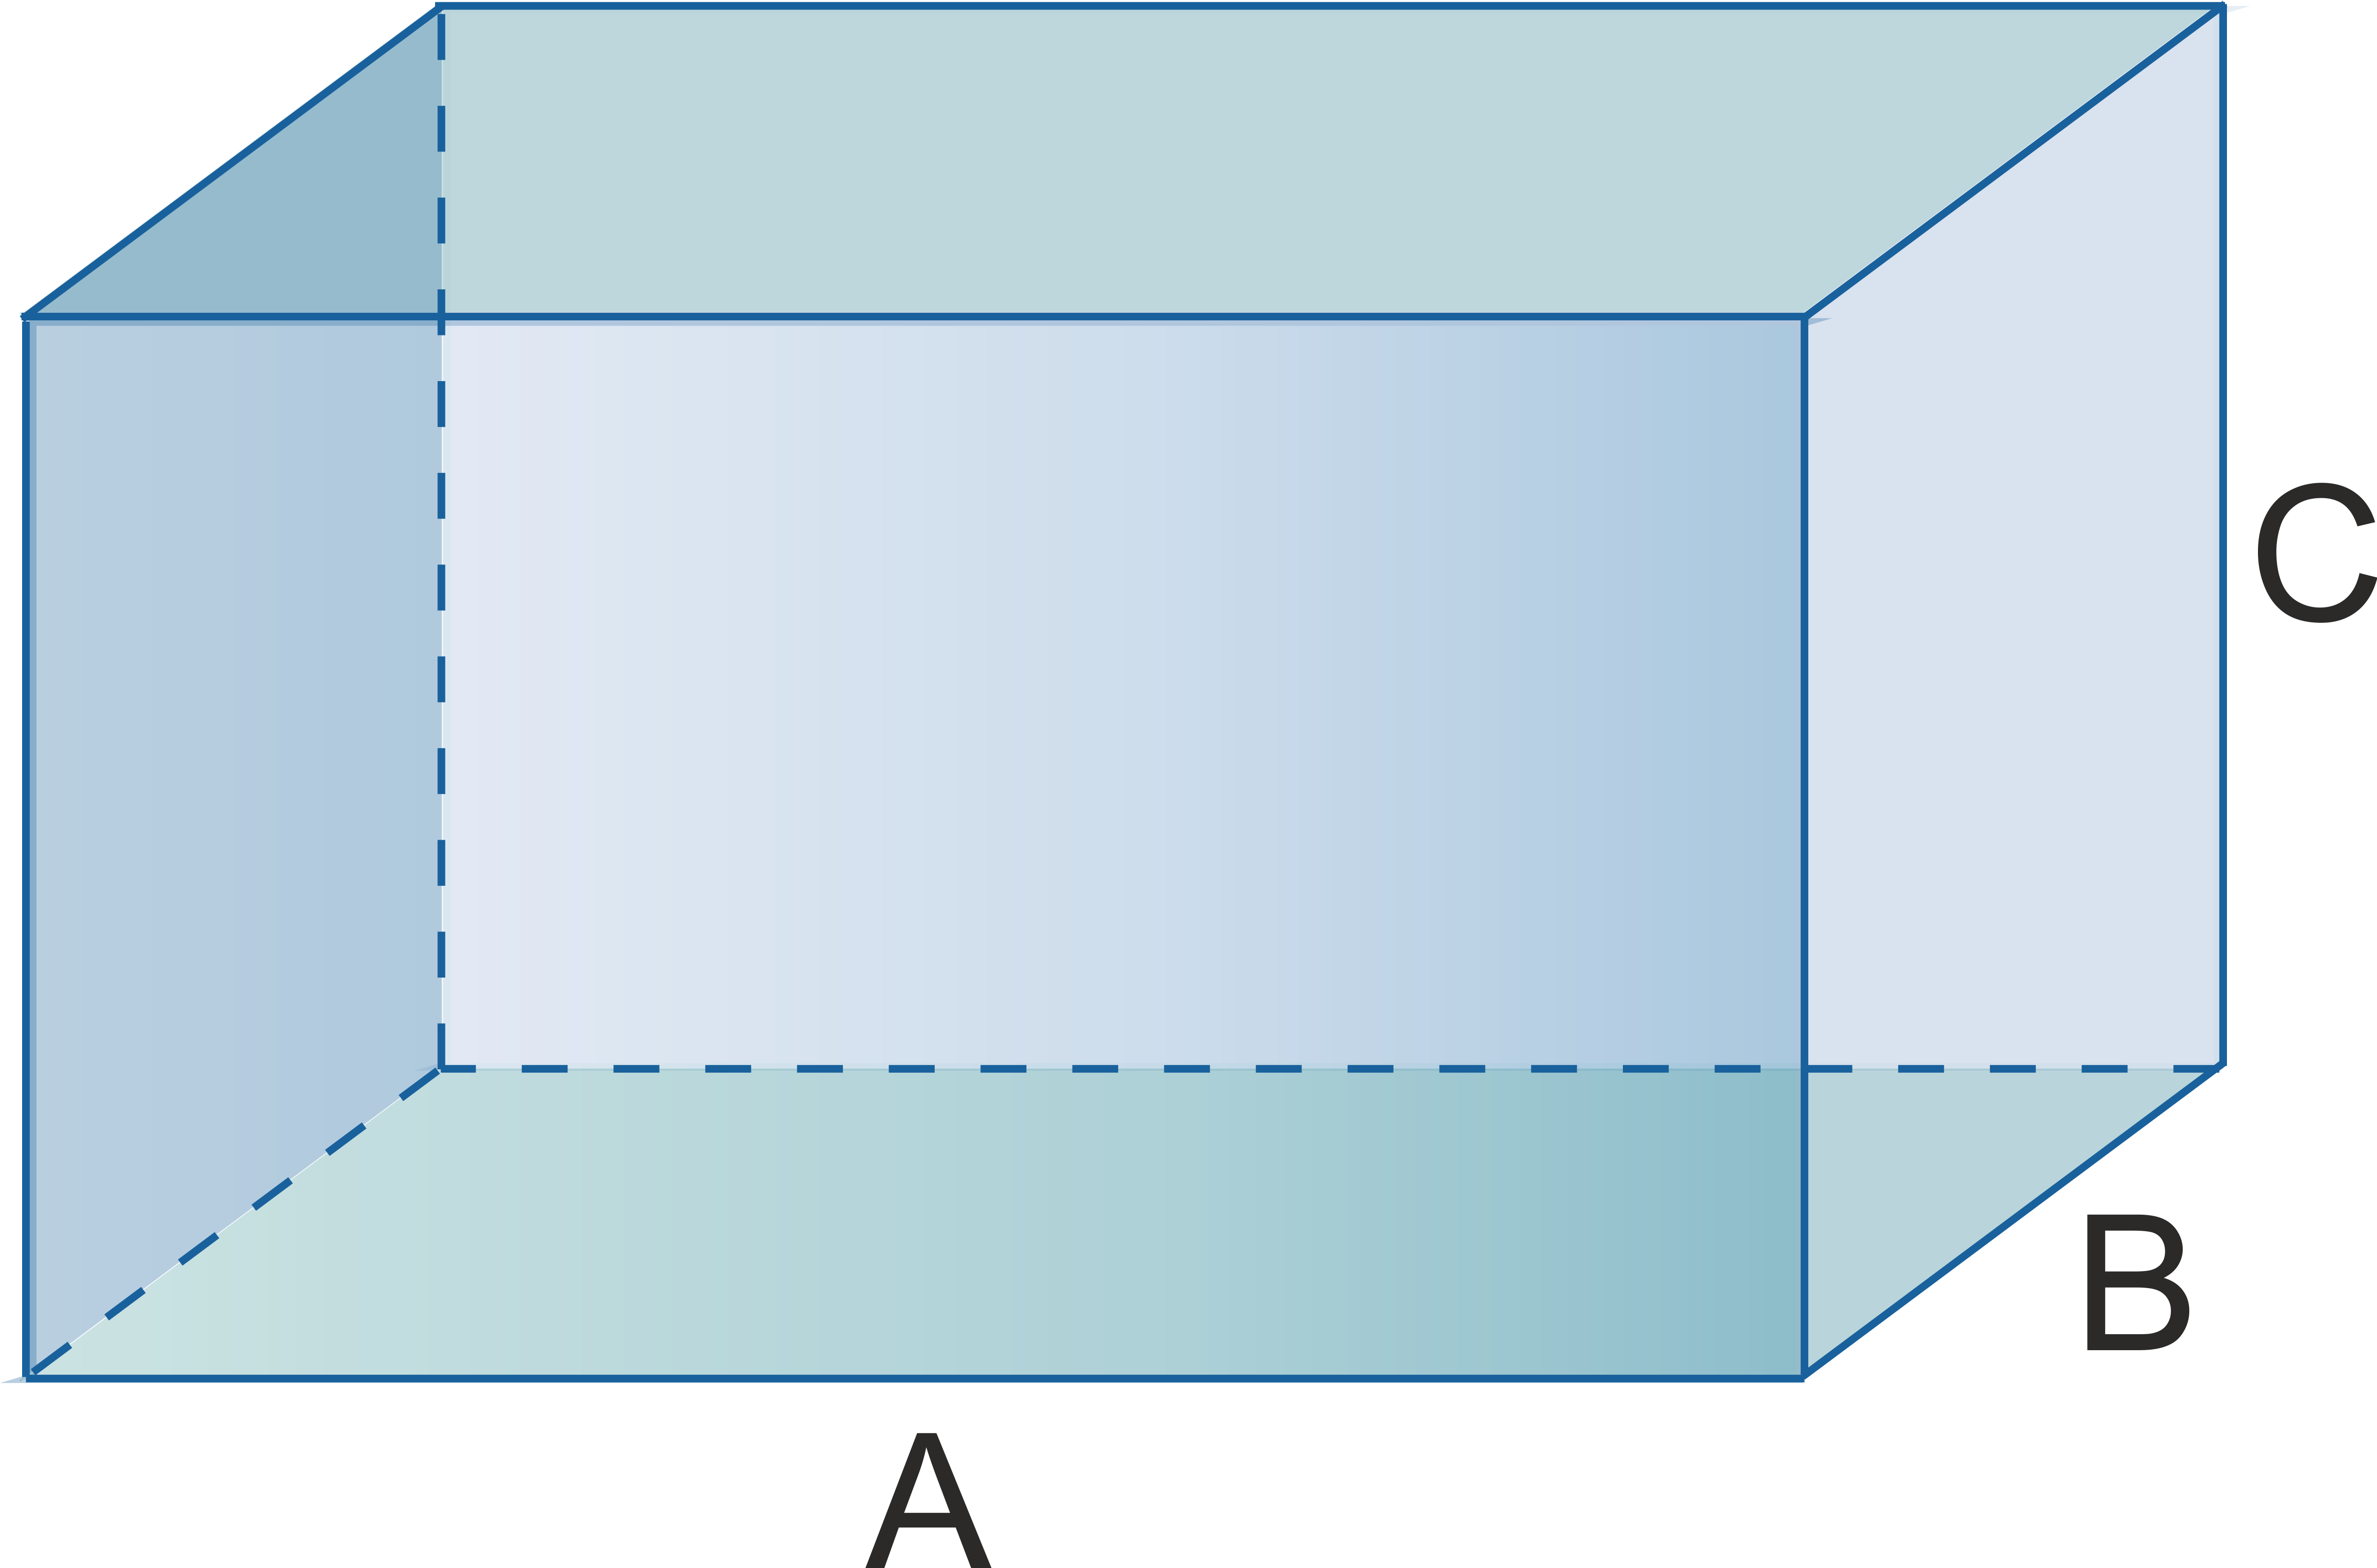
\includegraphics[width=0.75\textwidth]{../images/form_factor/anisotropic/rectangularparallelepiped.png}
\end{center}
\caption{Rectangular parallelepiped with edge lengths $A$, $B$, and $C$.}
\label{fig:recparallelepiped}
\end{figure}
The scattering intensity of a monodisperse randomly oriented rectangular parallelepiped with the edge lengths $A$, $B$, $C$, and a scattering length density contrast $\Delta\eta$ is given by
\begin{align}
\begin{split}
I_\text{rPE}(Q,A,B,C,\Delta\eta) = & \int\limits_0^\pi\int\limits_0^{\pi/2}
\frac{2}{\pi} \Bigg[ \textrm{sinc}\left(\frac{QA}{2} \sin(\alpha) \cos(\varphi)\right)  \\
				     &\textrm{sinc}\left(\frac{QB}{2} \sin(\alpha) \sin(\varphi)\right) \\
		             &\textrm{sinc}\left(\frac{QC}{2} \cos(\alpha)\right) ABC\, \Delta\eta \Bigg]^2  \sin\left(\alpha\right) \mathrm{d}\alpha \mathrm{d}\varphi
\end{split}
\end{align}
An additional size distribution is implemented in several ways either linearly, quadratically or cubically, depending if one two or all three axis scale with a single size distribution
\begin{align}
I_\text{rPE,1}(Q,\sigma, a, b,c,\Delta\eta) &= \int\limits_0^\infty \textrm{LogNorm}(\nu,\sigma) I_\text{rPE}(Q,\nu a,b,c,\Delta\eta) \mathrm{d}\nu \\
I_\text{rPE,2}(Q,\sigma, a, b,c,\Delta\eta) &= \int\limits_0^\infty \textrm{LogNorm}(\nu,\sigma) I_\text{rPE}(Q,\nu a,\nu b,c,\Delta\eta) \mathrm{d}\nu \\
I_\text{rPE,3}(Q,\sigma, a, b,c,\Delta\eta) &= \int\limits_0^\infty \textrm{LogNorm}(\nu,\sigma) I_\text{rPE}(Q,\nu a,\nu b,\nu c,\Delta\eta) \mathrm{d}\nu
\end{align}
with
\begin{align}
\textrm{LogNorm}(\nu,\sigma) &= \frac{1}{\sqrt{2\pi}\sigma} \exp\left(-\frac{\ln^2(\nu)}{2\sigma^2}\right)
\end{align}

\vspace{5mm}

\noindent \underline{Input Parameters for model \texttt{Parallelepiped\_abc}:}\\
\begin{description}
\item[\texttt{A}] width $A$
\item[\texttt{B}] depth $B$
\item[\texttt{C}] hight $C$
\item[\texttt{dummy}] not used
\item[\texttt{eta}] scattering length density contrast $\Delta\eta$
\end{description}

\noindent \underline{Input Parameters for models \texttt{Parallelepiped\_abc1}, \texttt{Parallelepiped\_abc2}}, \underline{and \texttt{Parallelepiped\_abc3}:}\\
\begin{description}
\item[\texttt{A}] width $A$
\item[\texttt{B}] depth $B$
\item[\texttt{C}] hight $C$
\item[\texttt{sigma}] width parameter $\sigma$ assuming a LogNorm-distribution
\item[\texttt{eta}] scattering length density contrast $\Delta\eta$
\end{description}

\noindent\underline{Note:}
\begin{itemize}
\item None
\end{itemize}

\begin{figure}[htb]
\begin{center}
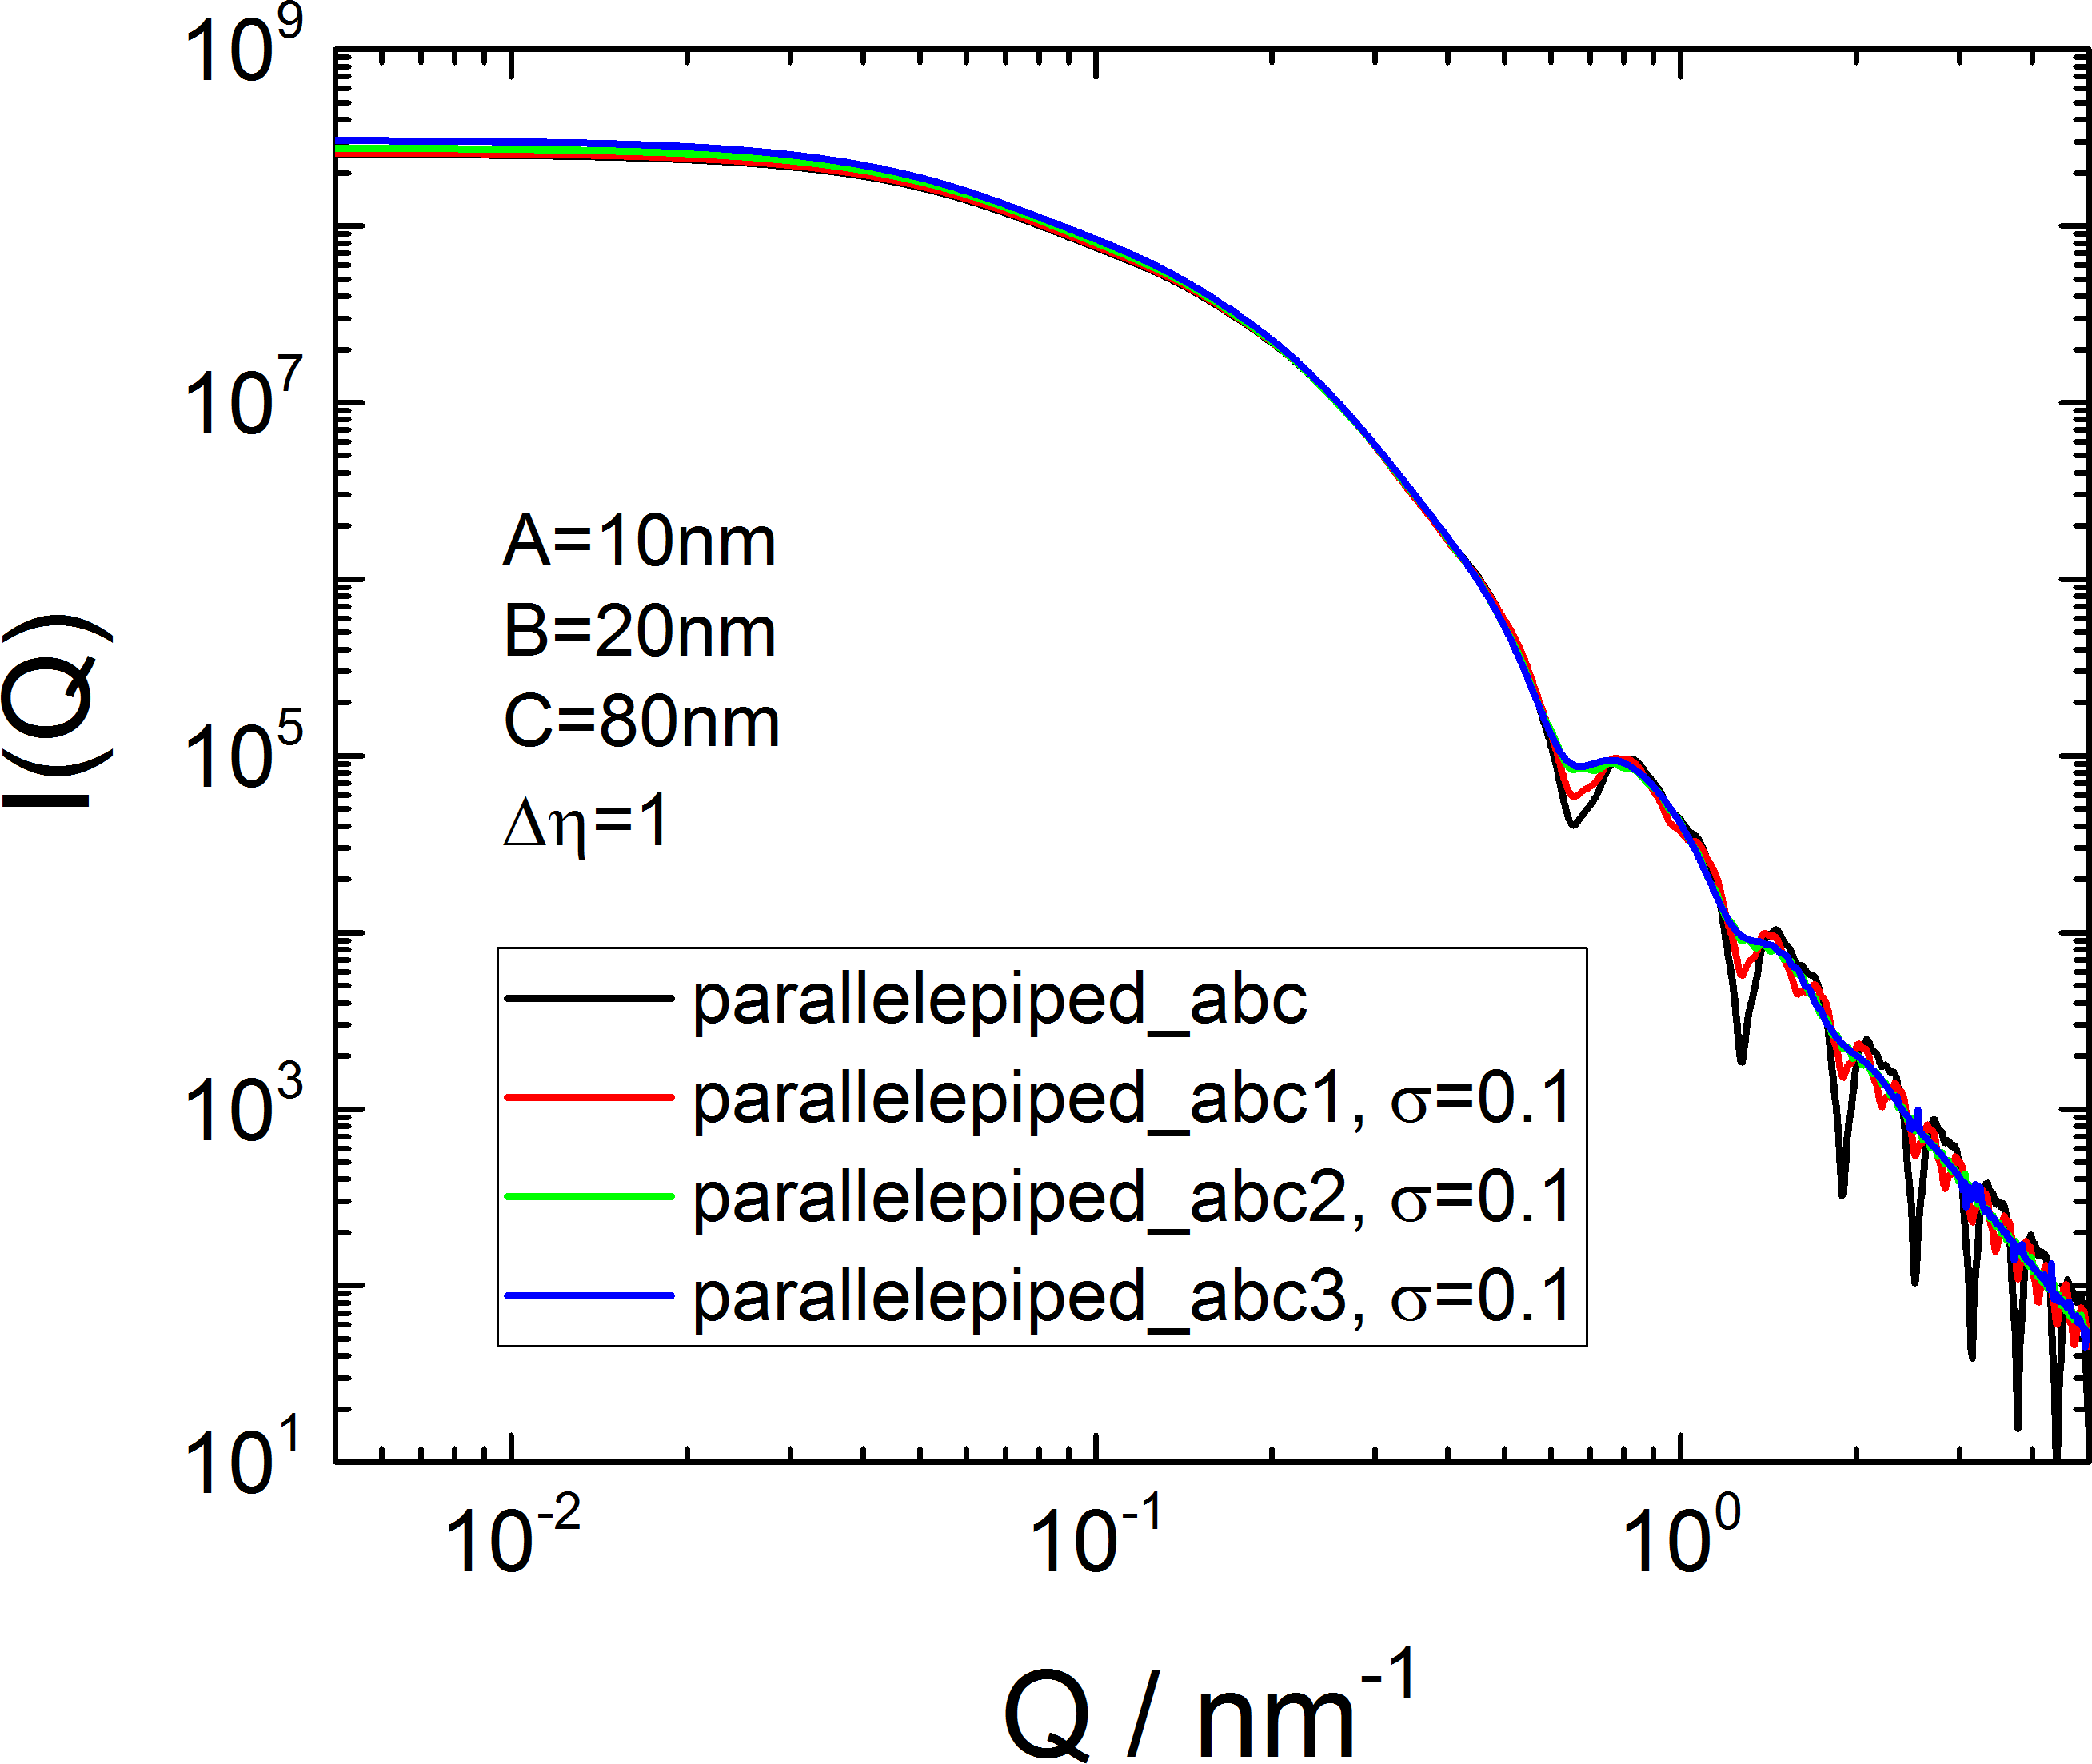
\includegraphics[width=0.75\textwidth]{../images/form_factor/anisotropic/parallelepipedABC.png}
\end{center}
\caption{Scattering curves for parallelepiped with optional size distribution a single edge length (\texttt{parallelepiped\_abc1}), of a surface area (\texttt{parallelepiped\_abc1}), or volume \texttt{parallelepiped\_abc3}.}
\label{fig:IQparallelepiped}
\end{figure}

%%%%%%%%%%%%%%%%%%%%%%%%%%%%%%%%%%%%%%%%%%%%%%%%%%%%%%%%%%%%%%%%%%%%%%%%%
\clearpage
\section{Very thin particles (local planar \& local cylindrical objects)}
\label{sec:very_anisotropic_particles}
For very thin random orientated particles the form factor
can be factorize according to Porod \cite{Porod1948} in a cross
section term $P_\text{cs}(Q)$ for the shorter or thin dimension and a
shape factor $P'(Q)$ for the long dimension.
\begin{align}
I(Q) &=P'(Q) P_{cs}(Q).
\end{align}
In this plugin the form factors of two types of thin
particles are collected, those with a local cylindrical and with a
local planar geometry. In case of local planar objects the cross
section term $P_\text{cs}(Q)$ can be homogeneous, a
centro-symmetric bilayer, a gaussian bilayer, etc. . This cross
section factor can than be combined with the overall shape factor
$P'(Q)$ of for examples a thin spherical shell of elliptical
shell, a thin cylindrical shell or a thin disc. As the total form
factor is the product of the cross-section form factor and a shape
form factor one can either programm all combination of
cross-section and shape factors into individual form factor
functions or one can programm the cross-section factors as form
factor and the shape factor as a structure factors. Using the
monodisperse approximation yields than the same result.

In this plugin the product of the cross-section and shape term
have been implemented as form factor under "\texttt{[by
plugin|thin obj.|local planar obj.]}" and "\texttt{[by
plugin|thin obj.|local cylindrical obj.]}". The
cross-section terms alone are also implemented as form factors
under "\texttt{[by plugin|thin obj.|Pcs(Q) for planar obj.]}"
and "\texttt{[by plugin|thin obj.|Pcs(Q) for cylindrical
obj.]}". The shape factors are also available as structure factors
under "\texttt{[by plugin|thin obj.|P'(Q): local planar
obj.]}" and "\texttt{[by plugin|thin obj.|P'(Q): local
cylindrical obj.]}".

The cross-section form factors can be easily calculated if the
scattering length density contrast profile
$\Delta\eta_\textrm{cs}(r)$ is known. For structures with a local
planar geometry and a symmetric cross-section the form factor is
given by
\begin{align}
P_\textrm{cs}^\textrm{planar} (Q) = \left[2\int_0^\infty
\Delta\eta_\textrm{cs}(r) \cos(Qr) \, \textrm{d}r\right]^2
\label{Pcs:planar}
\end{align}
In case of local cylindrical particles with a centro-symmetric
scattering length density distribution the form factor is given by
\begin{align}
P_\textrm{cs}^\textrm{cylindrical} (Q) = \left[2\pi\int_0^\infty
\Delta\eta_\textrm{cs}(r) \textrm{J}_0(Qr)r \,
\textrm{d}r\right]^2 \label{Pcs:cylindrical}
\end{align}

\clearpage
\subsection{Pcs(Q) for planar obj.} ~\\
\label{plugin:Pcs4planar}

The cross-section form factors with local planar geometry are valid
when the cross-section dimension is much smaller the radius of curvature
of the locally planar structure.
\begin{figure}[htb]
\begin{center}
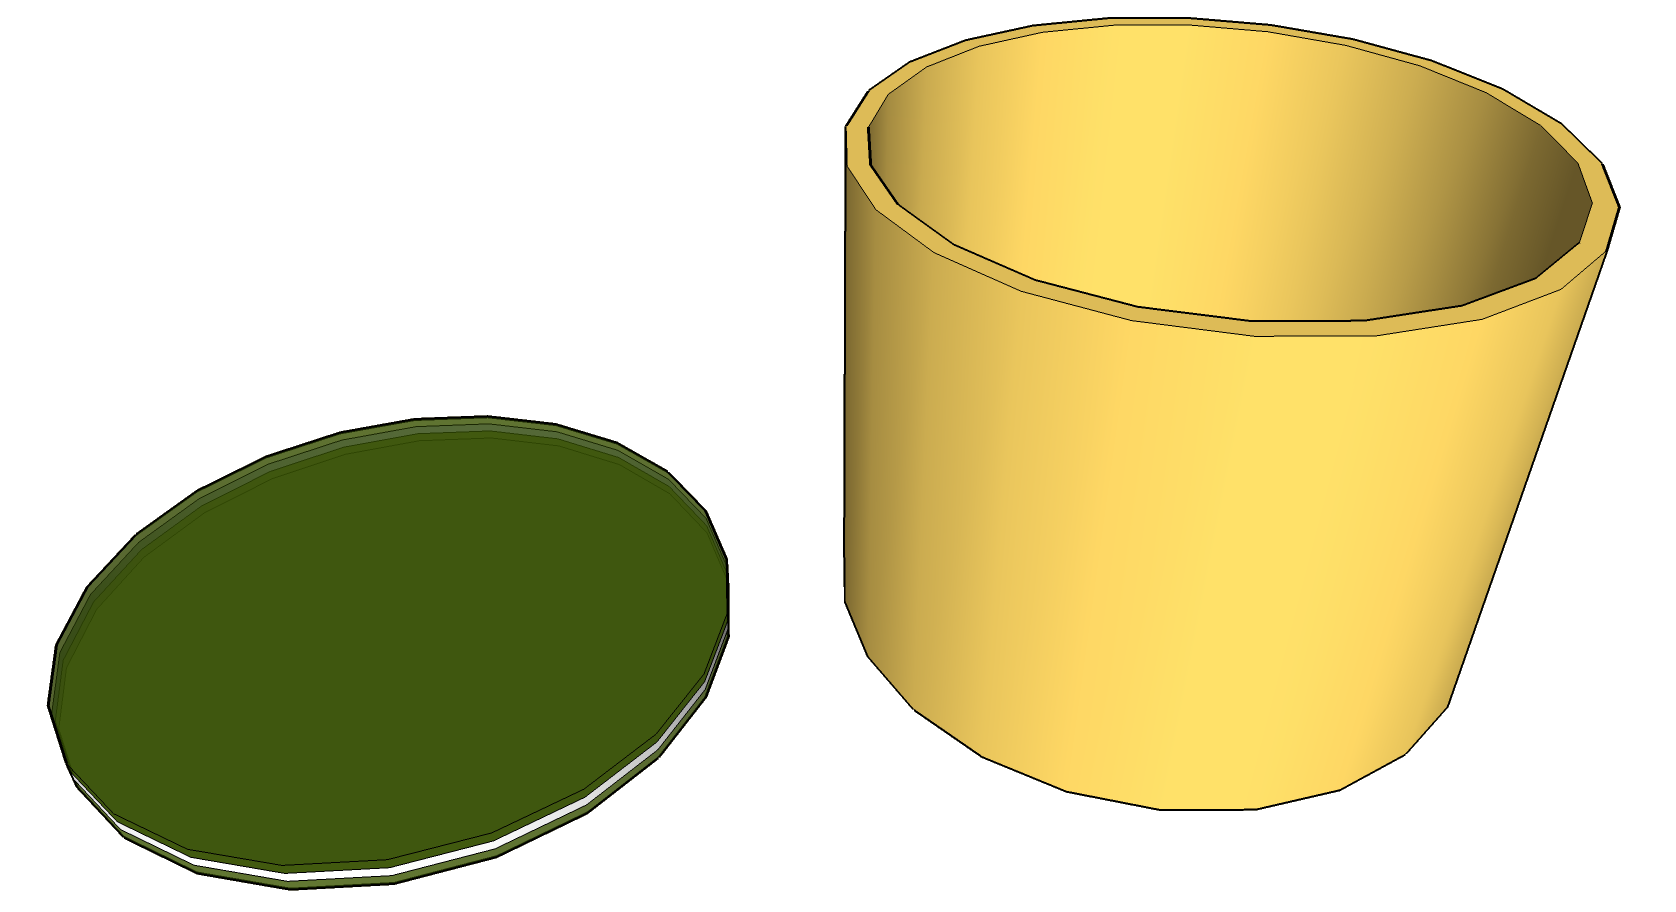
\includegraphics[width=0.838\textwidth,height=0.456\textwidth]{../images/form_factor/anisotropic/localplanar.png}
\end{center}
\caption{for local planar particles the cross section dimension is much smaller then the
radius of curvature of the particle}
\label{fig:localplanar}
\end{figure}

Several cross-section profiles for local planar objects have been implemented,
like a homogeneous cross-section,
cross-section with two infinitely thin plates,
layered centro-symmetric cross-section,
bilayer with a Gaussian scattering length density profile,
layer with Gaussian chains attached to the surface.
These form factors are supposed to be combined with a shape factor for
local planar objects which are implemented as structure  plugins
under "\texttt{[by plugin|thin obj.|P'(Q): local planar
obj.]}".

\clearpage

\subsubsection{Pcs(Q) for a homogeneous cross-section}
\label{plugin:Pcs:homogeneousXS} ~\\

\begin{figure}[htb]
\begin{center}
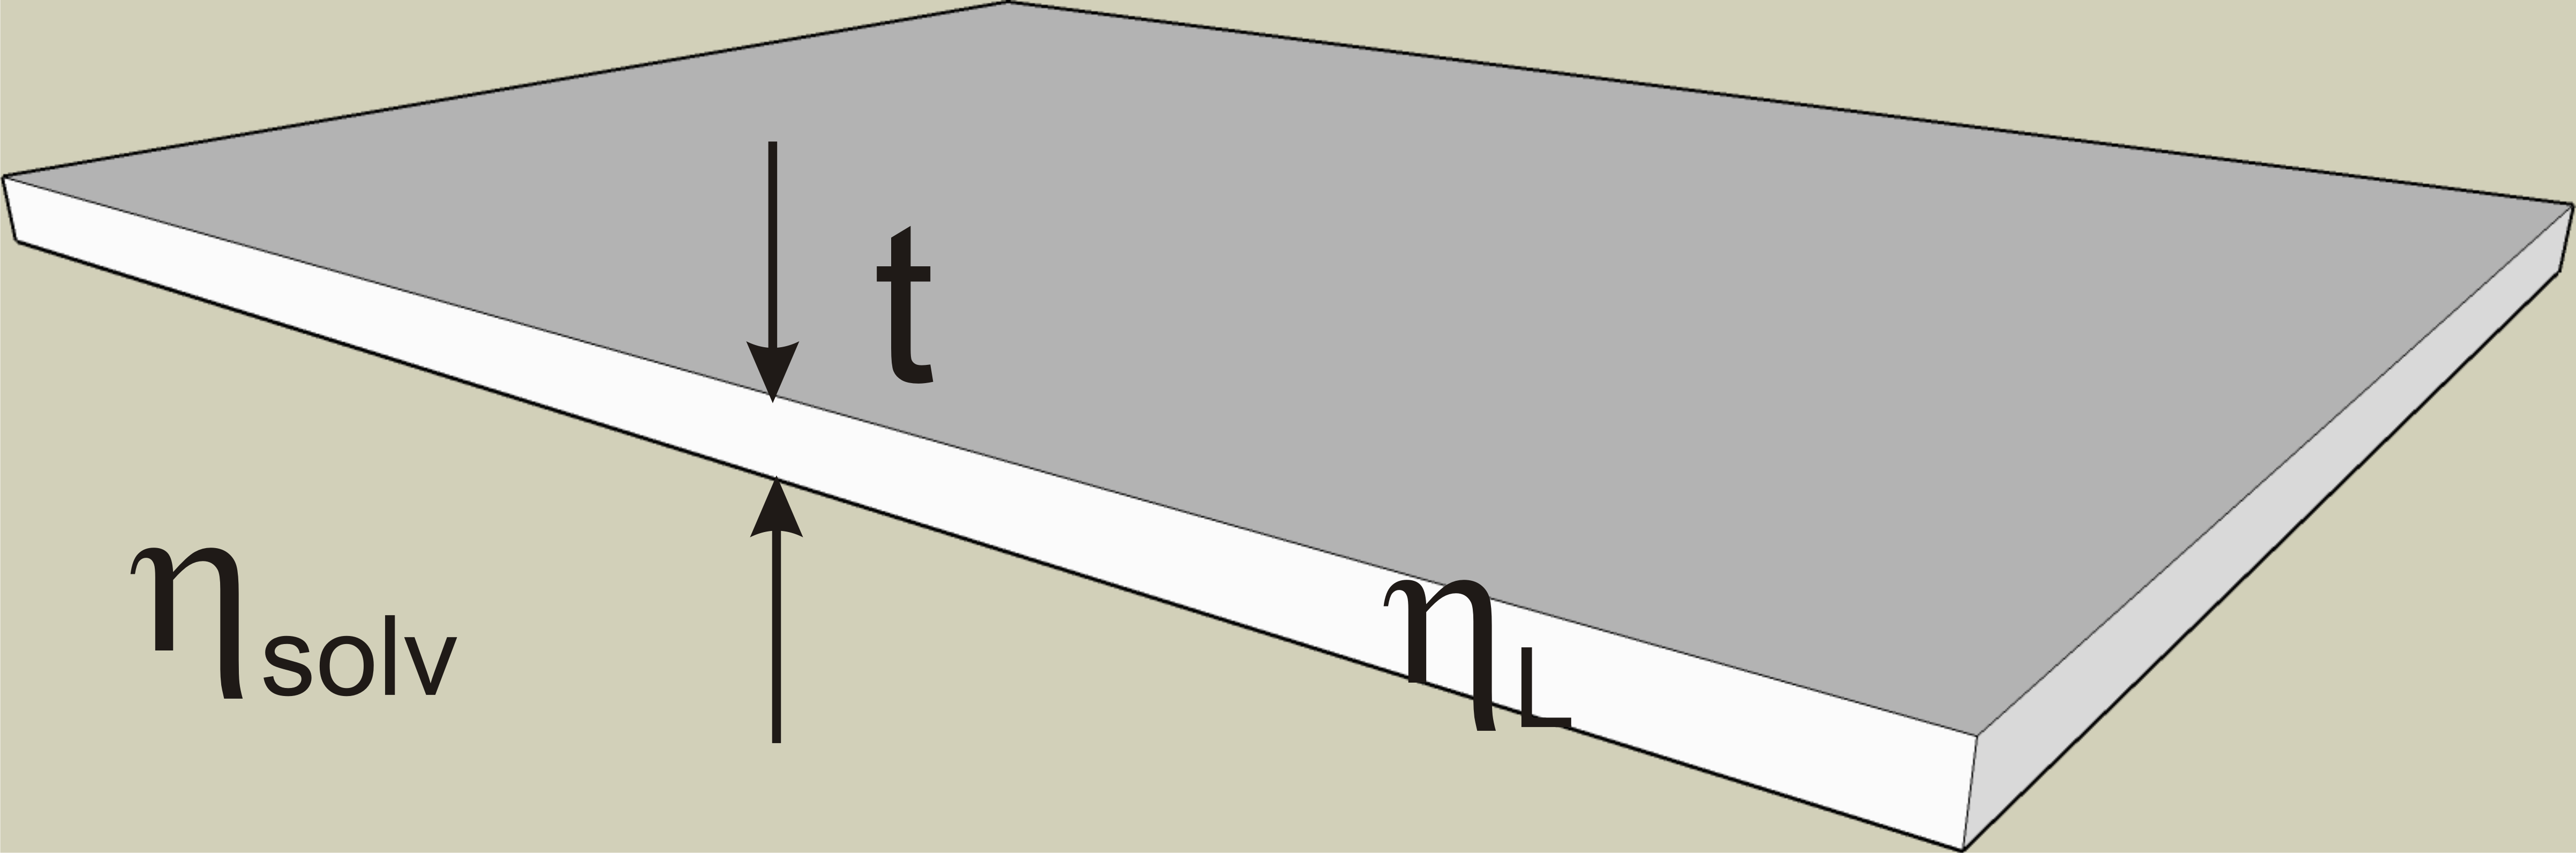
\includegraphics[width=0.802\textwidth,height=0.265\textwidth]{../images/form_factor/anisotropic/Pcs_homogeneousXS_txt.png}
\end{center}
\caption{Plane with a homogeneous cross-section of thickness $t$.}
\label{fig:homogeneousXS}
\end{figure}

This cross-section form factor describes the scattering of a layer with homogeneous
scattering length density $\eta_L$ in a matrix of a scattering length density $\eta_\textrm{solv}$.
The thickness can have a distribution described by a log-normal distribution according to eq.\ \ref{eq:LogNormal}.

\begin{align}
P_\text{cs}(Q,\sigma_{t},t) = \int_0^\infty \textrm{LogNorm}(x,1,\sigma_{t},1,t)
    \left[ \left(\eta_L-\eta_\textrm{solv}\right) x \frac{\sin(Qx/2)}{Qx/2} \right]^2\textrm{d}x
\label{eq:PcsHomogeneousPlate}
\end{align}

\vspace{5mm}

\hspace{1pt}\\
\underline{Input parameters for \texttt{Pcs:homogeneousPlate}:}
\begin{description}
    \item[\texttt{t}] most probable layer thickness $t$
    \item[\texttt{sigm\_t}] width $\sigma_t$ of thickness distribution (LogNorm)
    \item[\texttt{dummy}] unused disabled parameter
    \item[\texttt{dummy}] unused disabled parameter
    \item[\texttt{eta\_l}] scattering length density of layer $\eta_L$
    \item[\texttt{eta\_solv}] scattering length density of solvent $\eta_\textrm{solv}$
\end{description}

\noindent
\underline{Note}
\begin{itemize}
  \item This form factor is supposed to be combined with a shape factor for
local planar objects which are implemented as structure  plugins
under "\texttt{[by plugin|thin obj.|P'(Q): local planar
obj.]}".
\item As the form factor already have the width distribution included one normally uses in \SASfit as a size distribution
the \texttt{Delta}-distribution.
\end{itemize}

\begin{figure}[htb]
\begin{center}
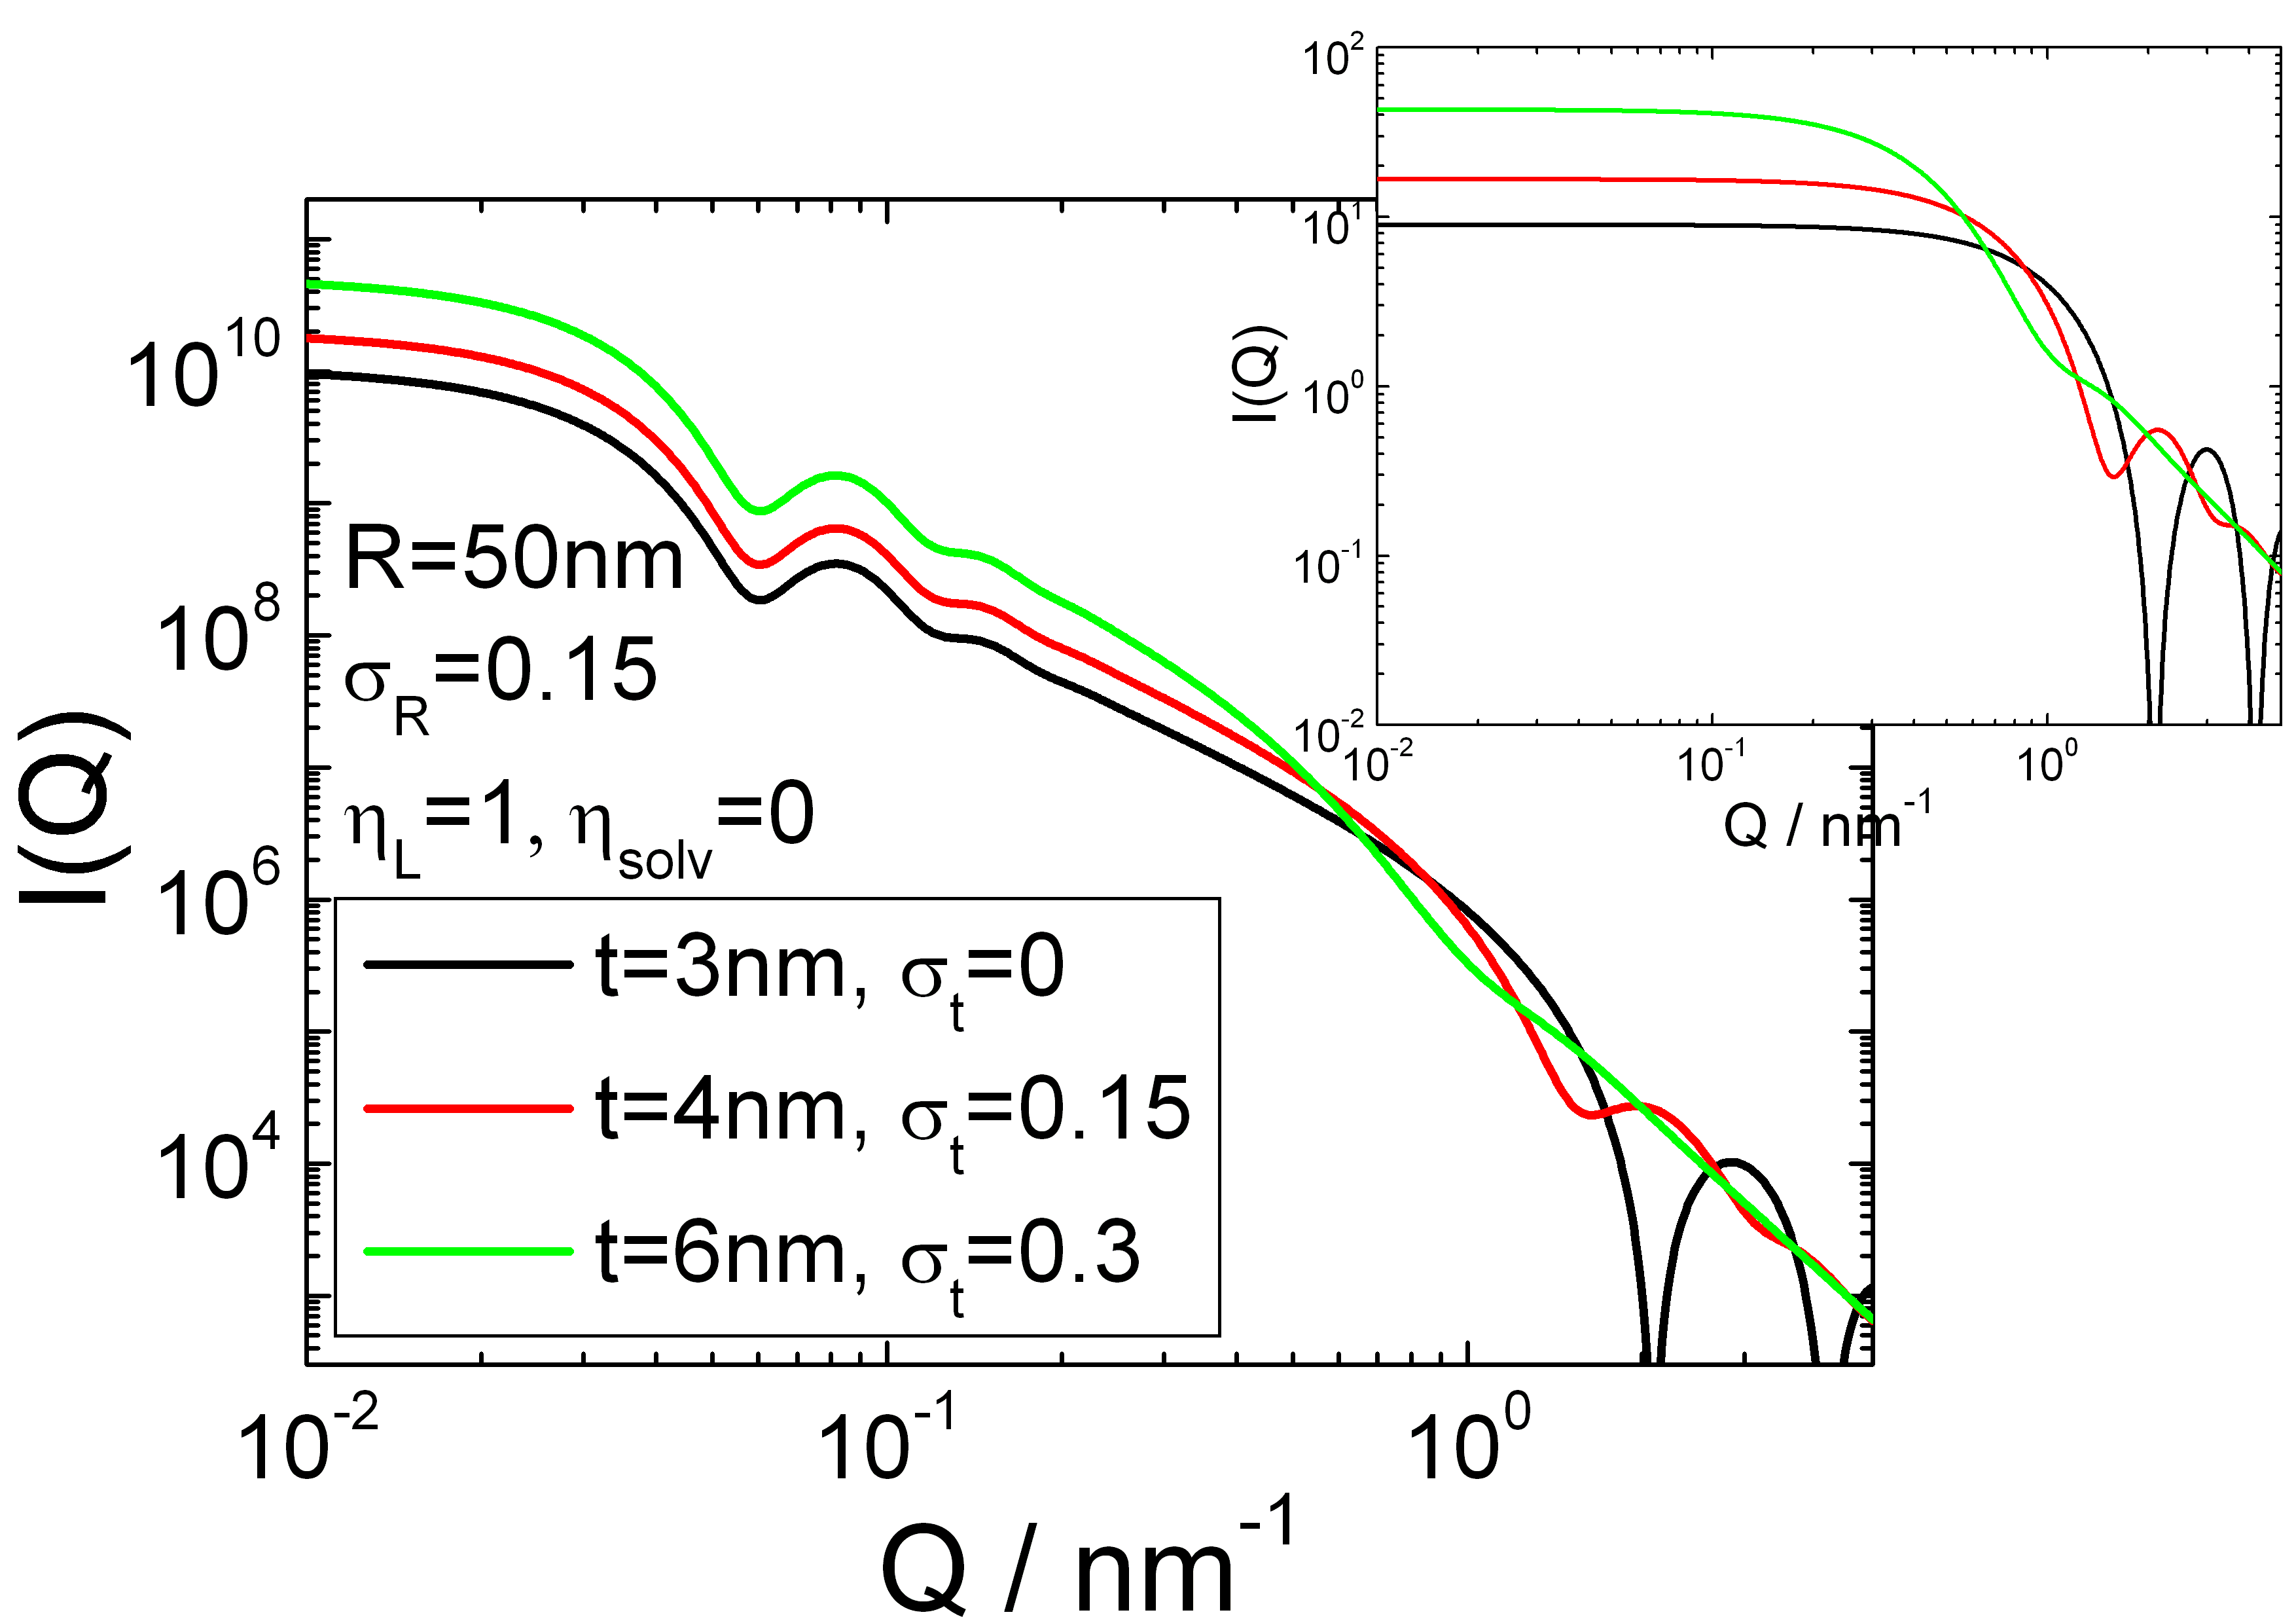
\includegraphics[width=0.8\textwidth,height=0.55\textwidth]{../images/form_factor/anisotropic/localplanarIQ.png}
\end{center}
\caption{Scattering curve for the form factor "\texttt{Pcs:homogeneousPlate}" only (insert) and
in combination with a structure factor "\texttt{P'(Q): Thin Spherical Shell}".}
\label{fig_IQ:homogeneousXS}
\end{figure}

\clearpage
\subsubsection{Pcs(Q) for two infinitely thin parallel layers} ~\\
\label{plugin:Pcs:TwoInfinitelyThinLayers}

\begin{figure}[htb]
\begin{center}
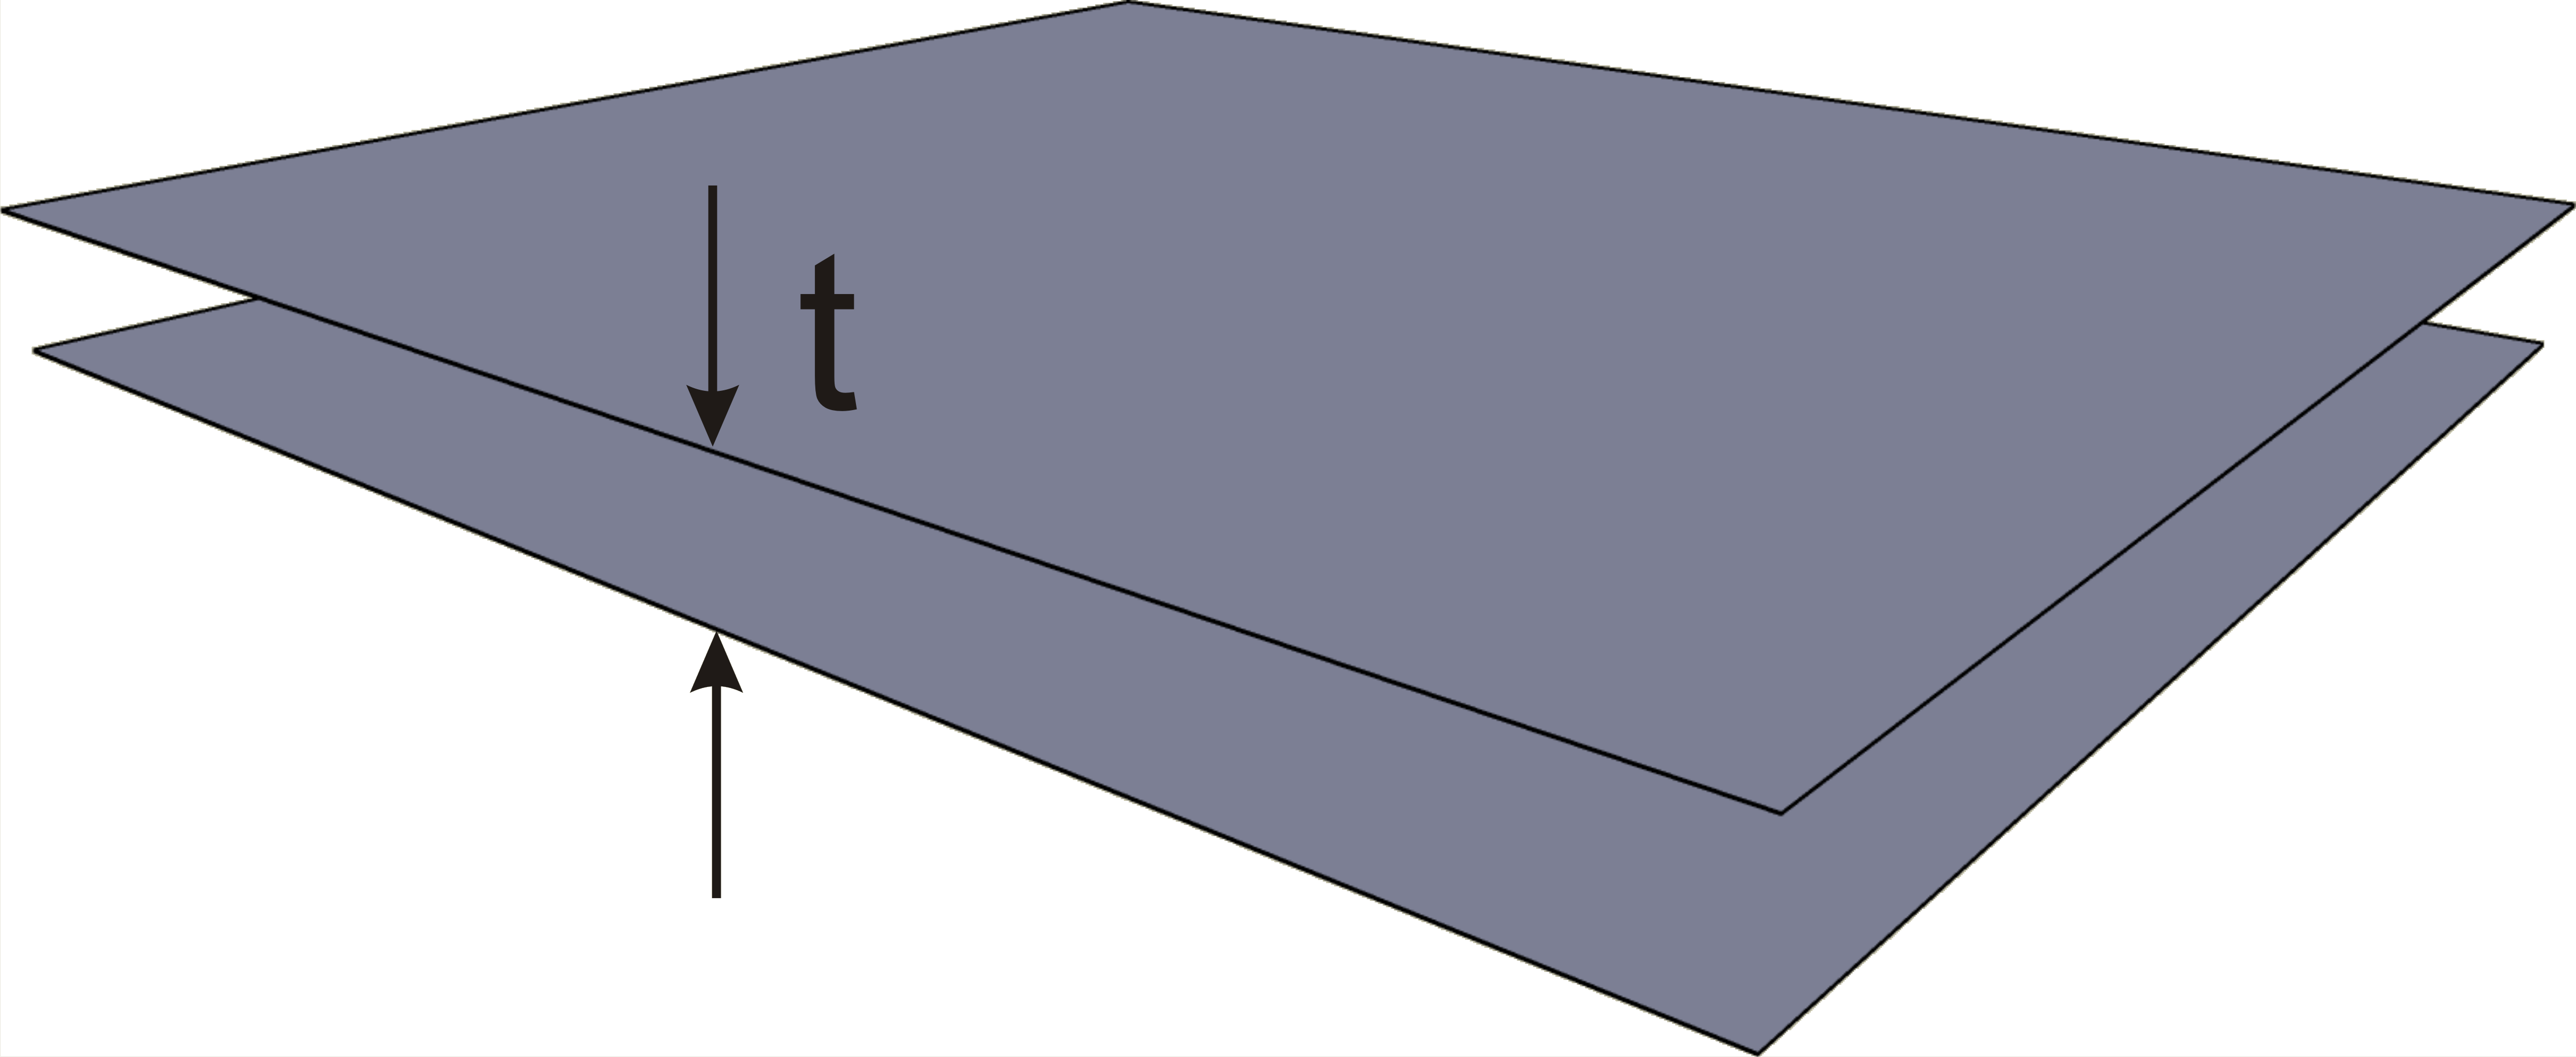
\includegraphics[width=0.8\textwidth,height=0.328\textwidth]{../images/form_factor/anisotropic/planar2thin_txt.png}
\end{center}
\caption{Two infinitely thin parallel layers separated by a distance $t$.}
\label{fig:Pcs:TwoInfinitelyThinLayers}
\end{figure}

This cross-section form factor describes the scattering of two infinitely thin parallel layers.
The separation distance can have a distribution described by a log-normal distribution according
to eq.\ \ref{eq:LogNormal}.

\begin{align}
P_\text{cs}(Q,\sigma_{t},t) = \int_0^\infty \textrm{LogNorm}(x,1,\sigma_{t},1,t) \cos^2(Qx/2) \, \textrm{d}x
\end{align}

\vspace{5mm}

\hspace{1pt}\\
\underline{Input parameters for \texttt{Pcs:TwoInfinitelyThinLayers}:}
\begin{description}
    \item[\texttt{t}] most probable layer separation $t$
    \item[\texttt{sigm\_t}] width $\sigma_t$ of separation distribution (LogNorm)
\end{description}

\noindent
\underline{Note}
\begin{itemize}
  \item This form factor is supposed to be combined with a shape factor for
local planar objects which are implemented as structure  plugins
under "\texttt{[by plugin|thin obj.|P'(Q): local planar
obj.]}".
\item As the form factor already have the width distribution included one normally uses in \SASfit as a size distribution
the \texttt{Delta}-distribution.
\end{itemize}

\begin{figure}[htb]
\begin{center}
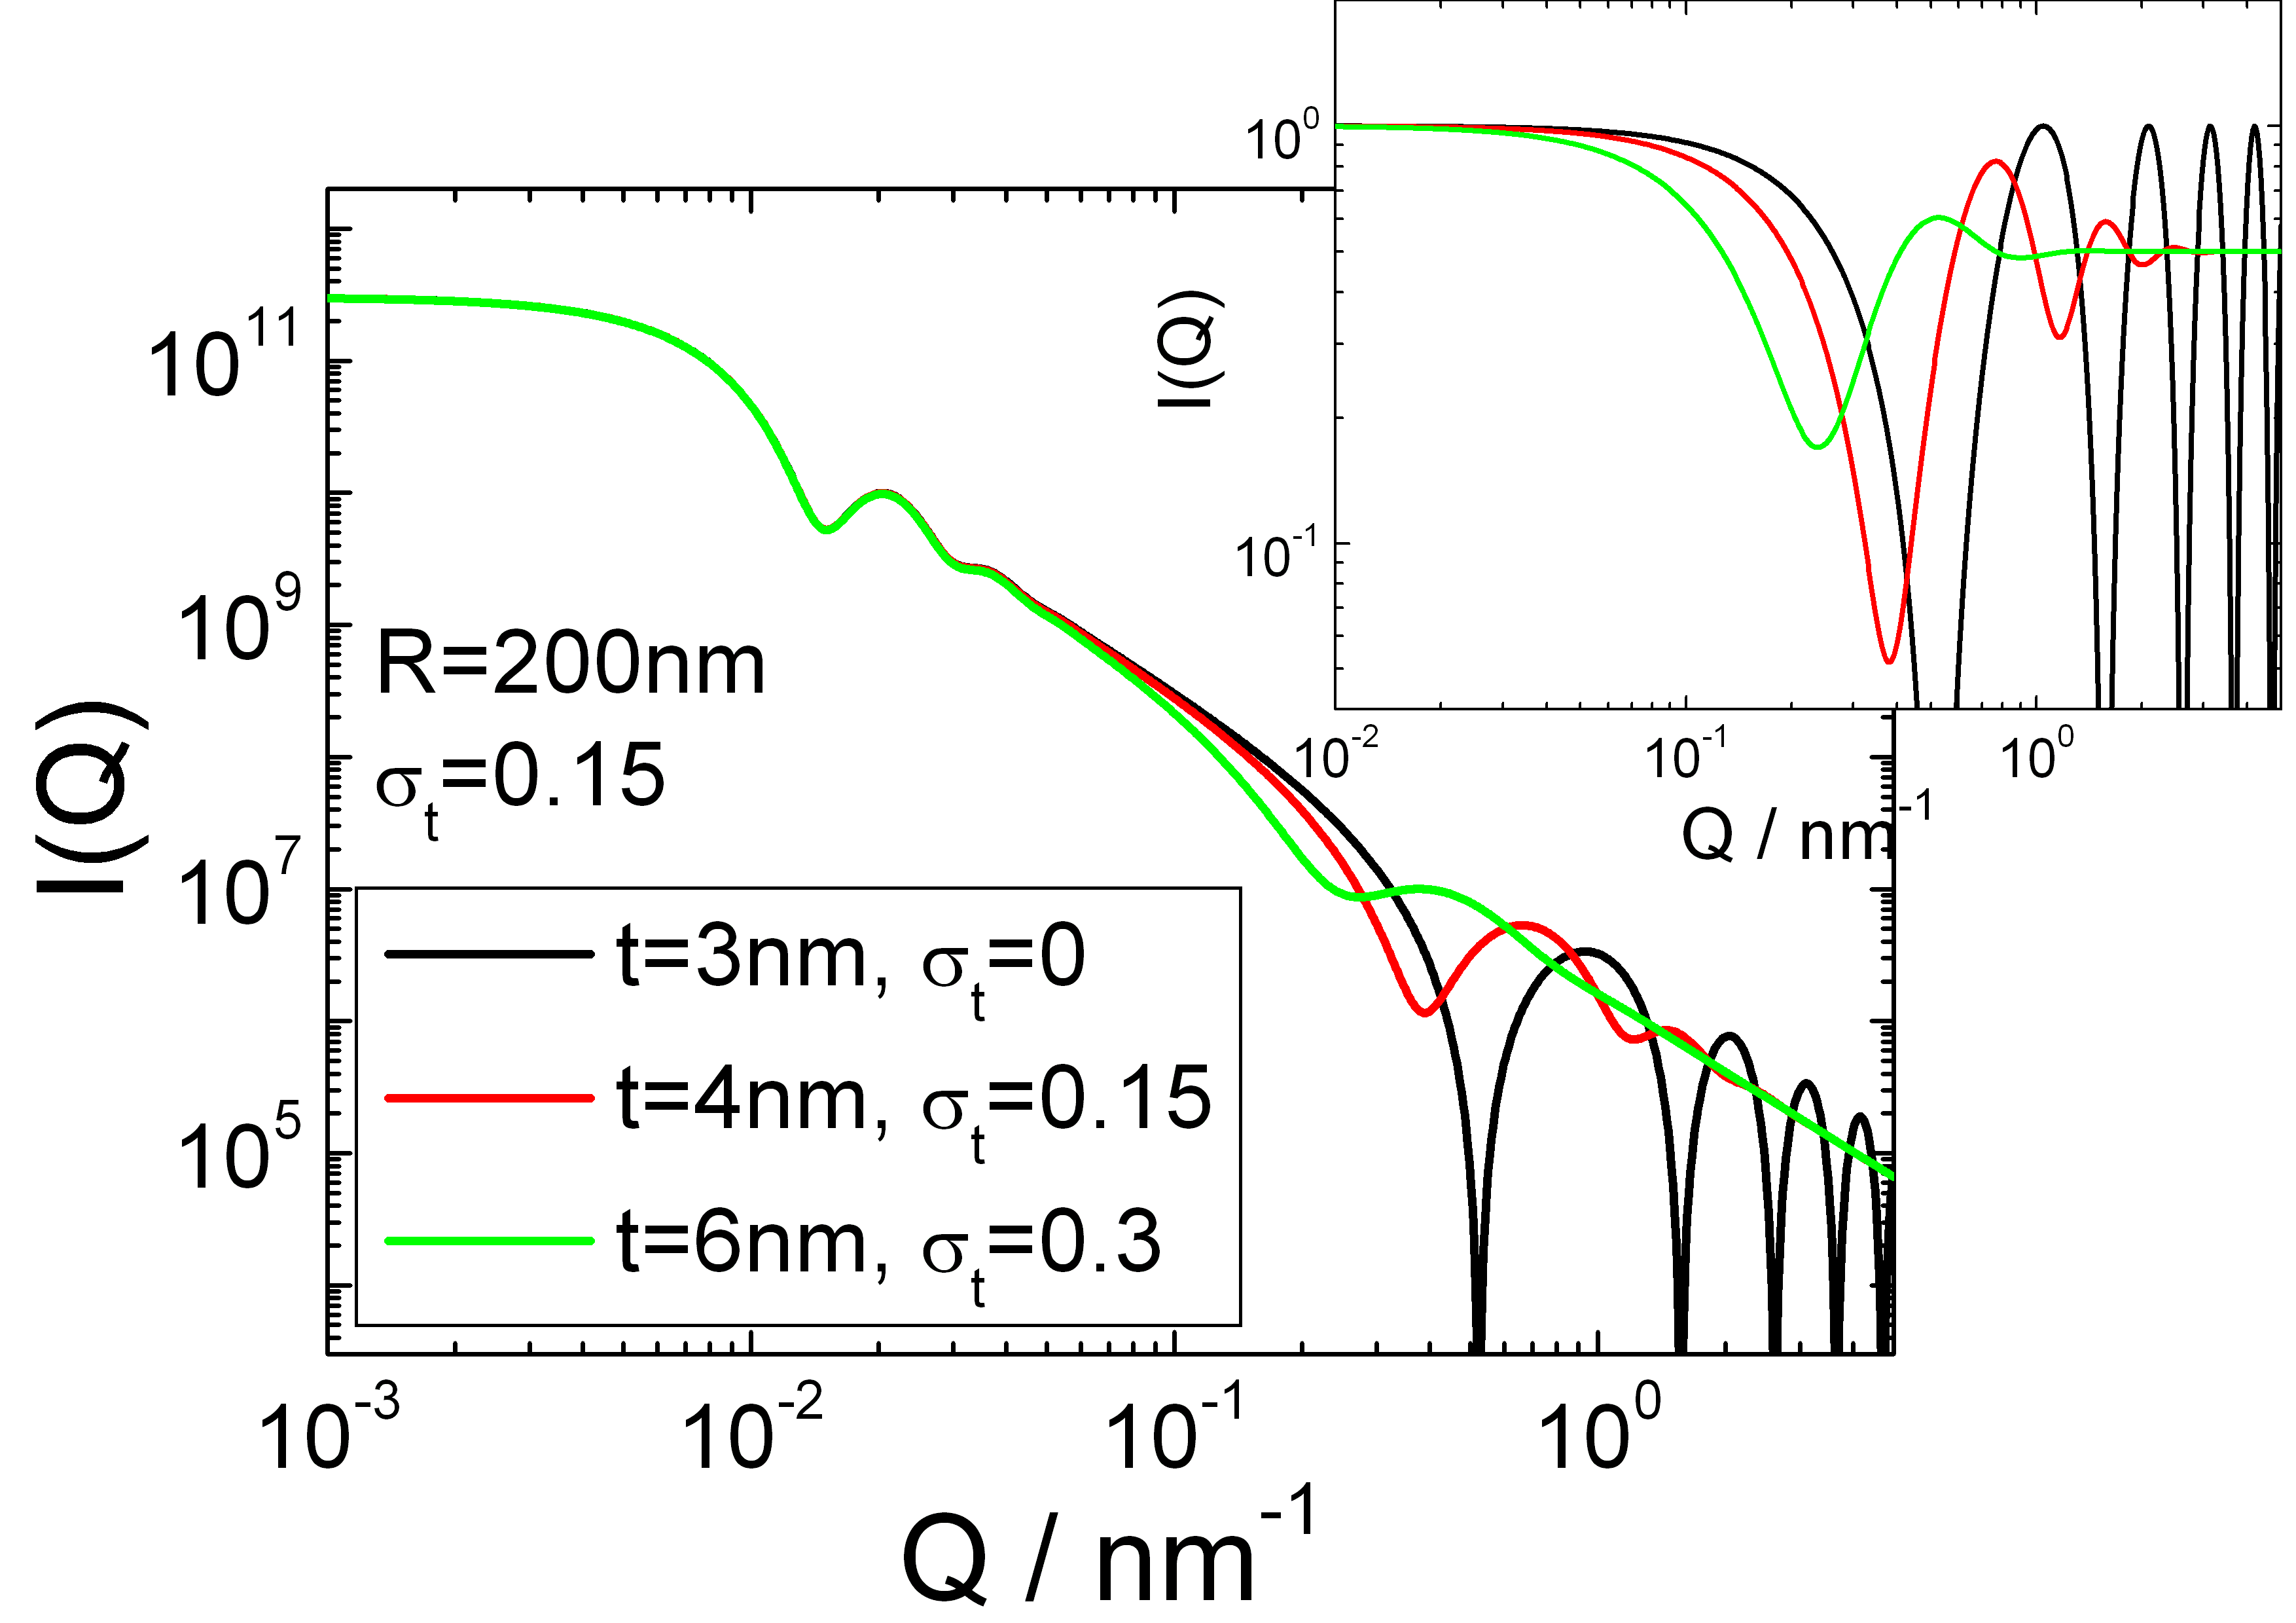
\includegraphics[width=0.8\textwidth,height=0.55\textwidth]{../images/form_factor/anisotropic/planar2thinIQ.png}
\end{center}
\caption{Scattering curve for the form factor "\texttt{Pcs:TwoInfinitelyThinLayers}" only (insert) and
in combination with a structure factor "\texttt{P'(Q): Thin Spherical Shell}".}
\label{fig_IQ:Pcs:TwoInfinitelyThinLayers}
\end{figure}


\clearpage
\subsubsection{Pcs(Q) for a layered centro symmetric cross-section structure} ~\\
\label{plugin:Pcs:LayeredCentroSymmetricCrossSectionStructure}

\begin{figure}[htb]
\begin{center}
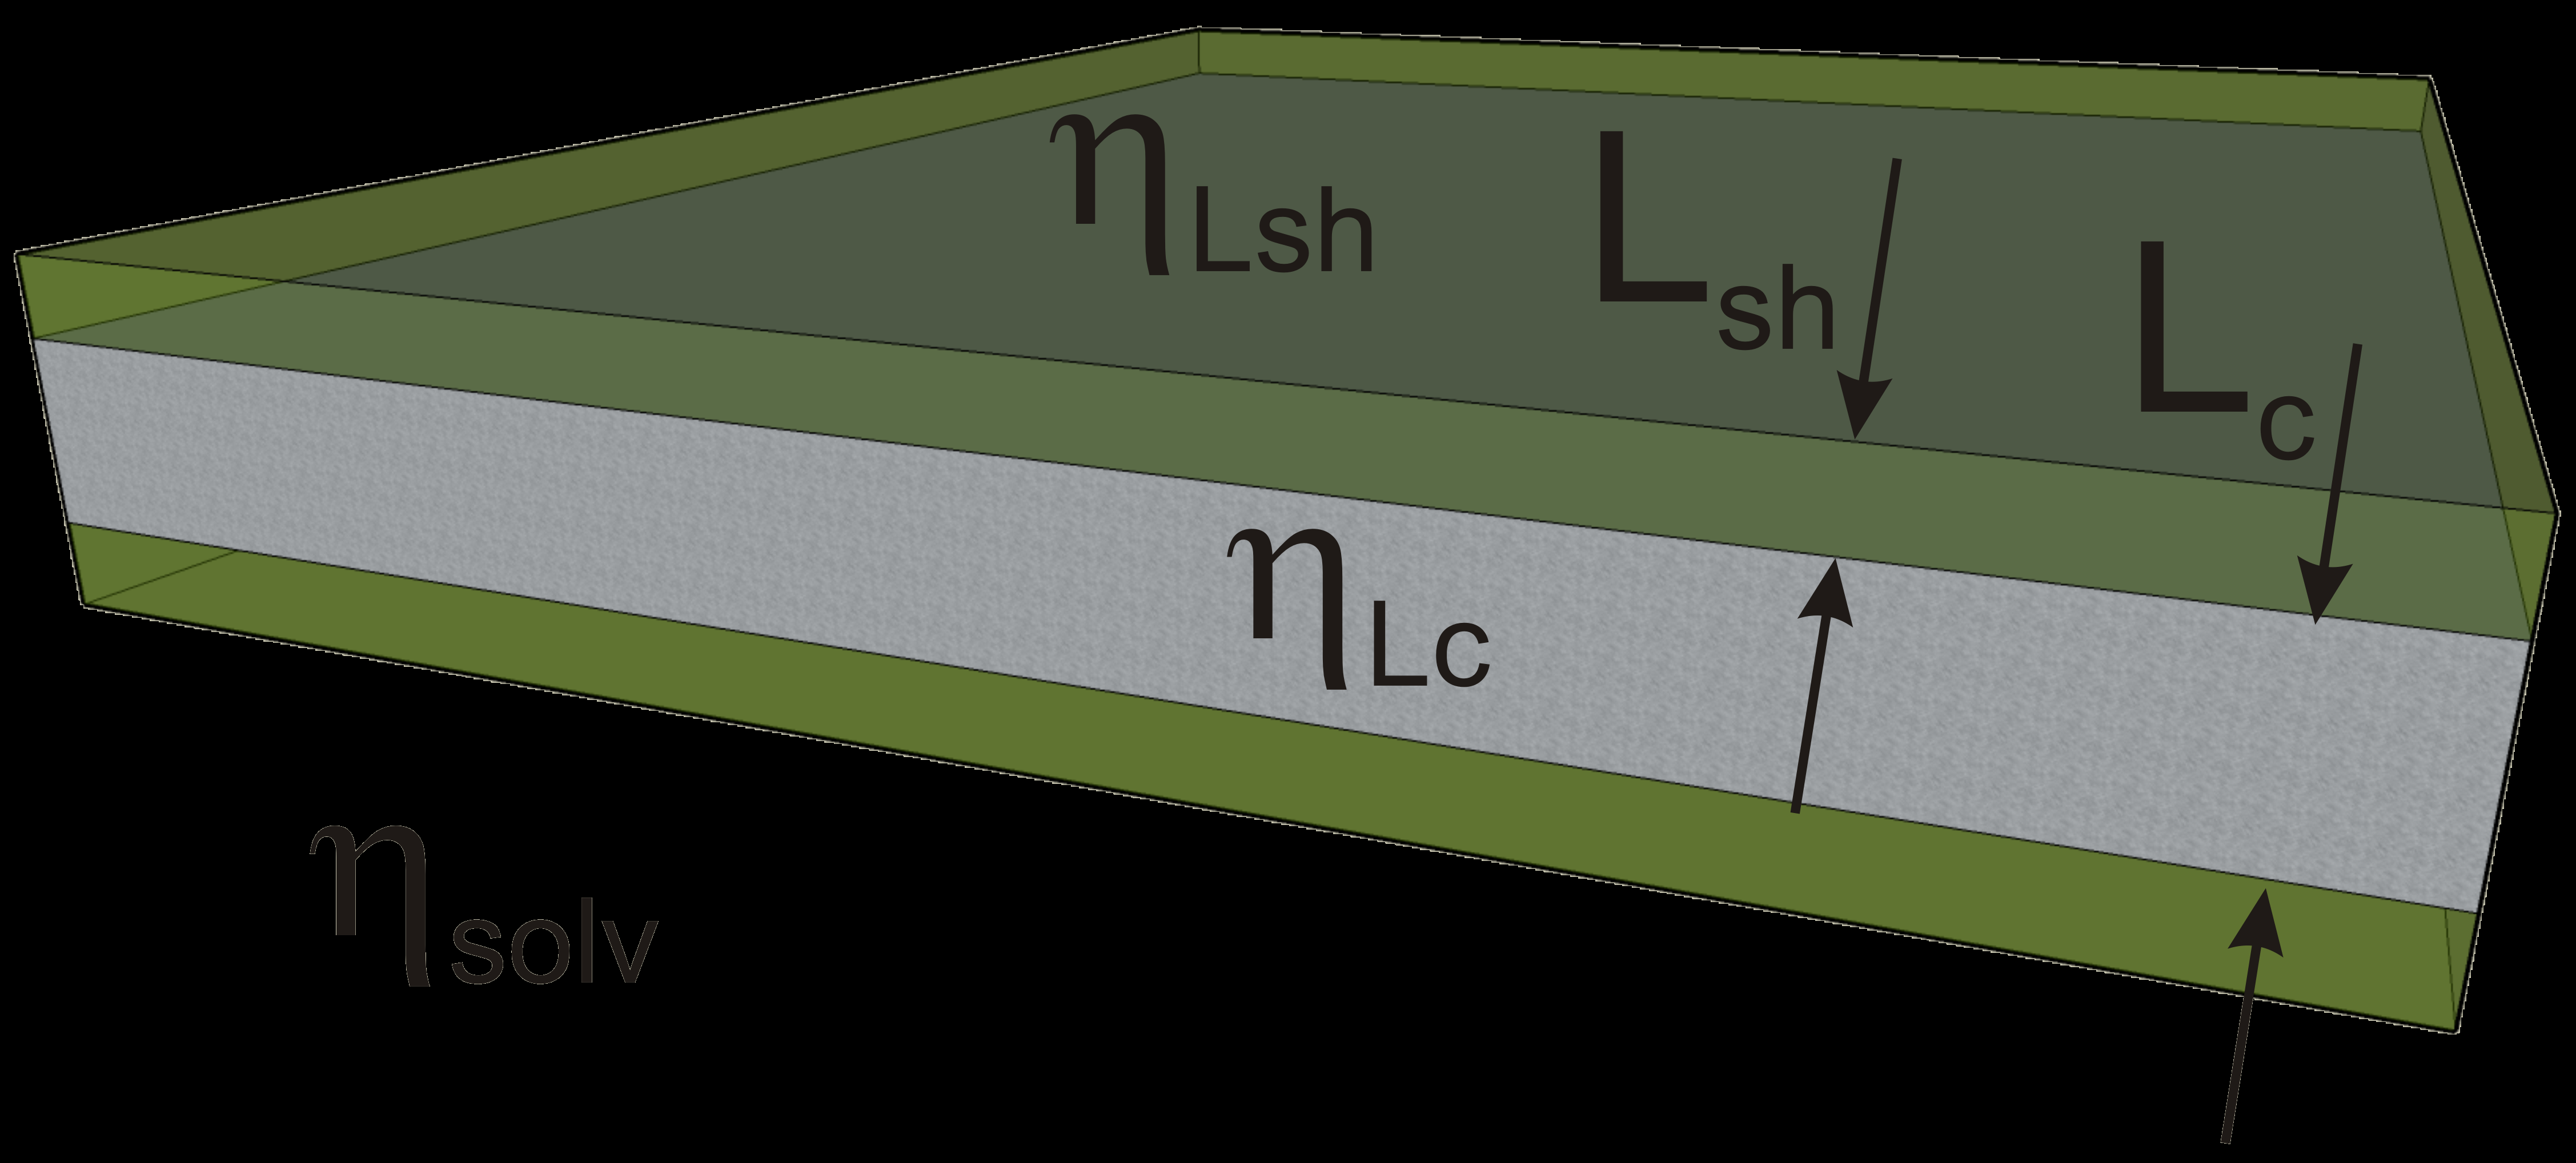
\includegraphics[width=0.8\textwidth,height=0.361\textwidth]{../images/form_factor/anisotropic/planar2centrosymm_txt.png}
\end{center}
\caption{Two layered centro symmetric structure with a core thickness of $L_\textrm{c}$ and an outer layer thickness
$L_{L_\textrm{sh}}$. The corresponding scattering length densities of the core, the shell layer and the solvent are
$L_{L_\textrm{c}}$, $L_{L_\textrm{sh}}$, and $L_{L_\textrm{solv}}$.}
\label{fig:Pcs:LayeredCentroSymmetricCrossSection}
\end{figure}

This cross-section form factor describes the scattering of a layered centro symmetric cross-section structure.
Both the core thickness as well as the shell thickness can have a distribution described by a log-normal distribution as defined in eq.\ \ref{eq:LogNormal}.

\begin{multline}
P_\text{cs}(Q,\sigma_{L_\textrm{c}},L_\textrm{c},\sigma_{L_\textrm{sh}},L_\textrm{sh},\eta_{L_\textrm{c}},\eta_{L_\textrm{sh}},\eta_\textrm{sol}) = \\
\int_0^\infty \textrm{LogNorm}(v,1,\sigma_{L_\textrm{c}},1,L_\textrm{c})
\int_0^\infty \textrm{LogNorm}(u,1,\sigma_{L_\textrm{sh}},1,L_\textrm{sh}) \\
     \Bigg[ \frac{(\eta_{L_\textrm{sh}}-\eta_\textrm{solv})(v+2u) \sin\left(Q\frac{v+2u}{2}\right)}{Q\frac{v+2u}{2}}
          -\frac{(\eta_{L_\textrm{sh}}-\eta_{L_\textrm{c}})  v   \sin\left(Q \frac{v}{2}\right)}{Q \frac{v}{2}}
    \Bigg]^2 \,
\textrm{d}u \, \textrm{d}v
\end{multline}

\vspace{5mm}

\hspace{1pt}\\
\underline{Input parameters for \texttt{Pcs:LayeredCentroSymmetricXS}:}
\begin{description}
    \item[\texttt{L\_c}] most probable layer separation $L_\textrm{c}$
    \item[\texttt{sigm\_Lc}] width $\sigma_{L_\textrm{c}}$ of core thickness distribution (LogNorm)
    \item[\texttt{L\_sh}] most probable shell thickness $L_\textrm{sh}$
    \item[\texttt{sigm\_Lsh}] width $\sigma_{L_\textrm{c}}$ of shell thickness distribution (LogNorm)
    \item[\texttt{eta\_Lc}] scattering length density of core layer $\eta_{L_\textrm{c}}$
    \item[\texttt{eta\_Lsh}] scattering length density of shell layer $\eta_{L_\textrm{sh}}$
    \item[\texttt{eta\_solv}] scattering length density of solvent $\eta_{solv}$
\end{description}

\noindent
\underline{Note}
\begin{itemize}
  \item This form factor is supposed to be combined with a shape factor for
local planar objects which are implemented as structure  plugins
under "\texttt{[by plugin|thin obj.|P'(Q): local planar
obj.]}".
\item As the form factor already have the width distribution included one normally uses in \SASfit as a size distribution
the \texttt{Delta}-distribution.
\end{itemize}

\begin{figure}[htb]
\begin{center}
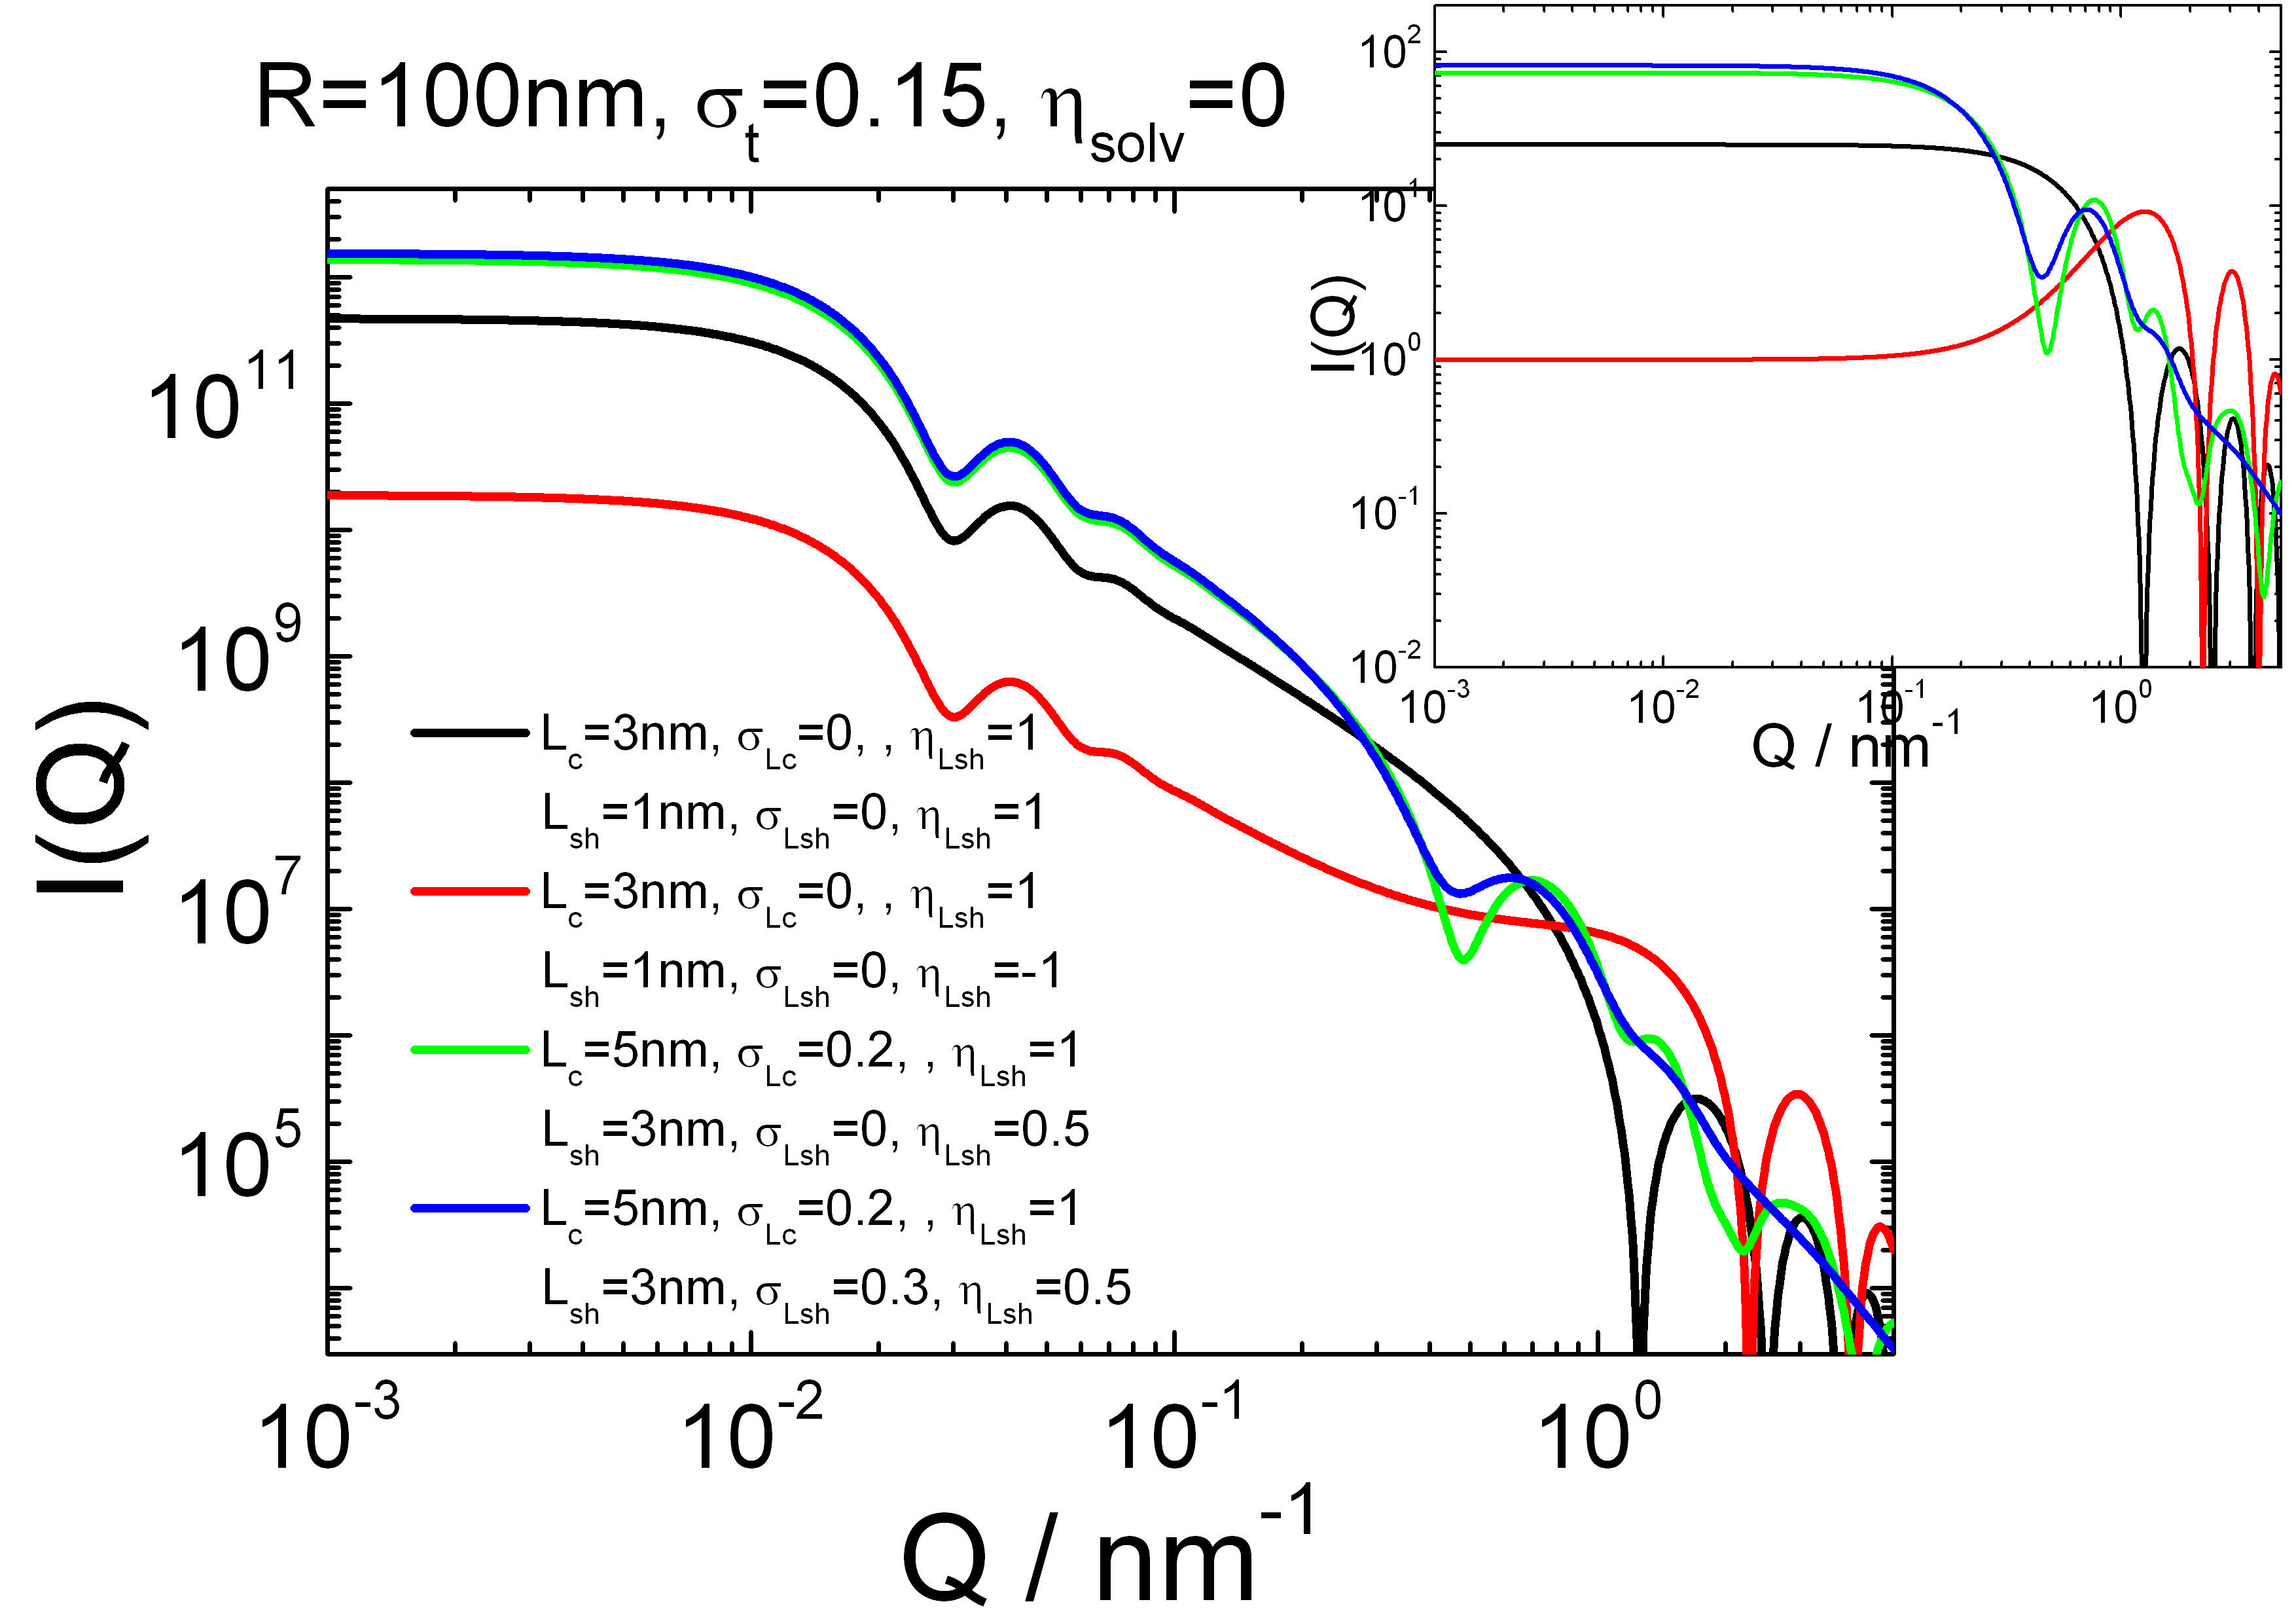
\includegraphics[width=0.8\textwidth,height=0.55\textwidth]{../images/form_factor/anisotropic/Pcs_planar2centrosymmIQ.png}
\end{center}
\caption{Scattering curve for the form factor "\texttt{Pcs:LayeredCentroSymmetricXS}" only (insert) and
in combination with a structure factor "\texttt{P'(Q): Thin Spherical Shell}".}
\label{fig:Pcs_planar2centrosymmIQ}
\end{figure}

\clearpage

\subsubsection{Pcs(Q) for a bilayer with a Gaussian electron density profile \cite{Pabst2000,Pabst2003}} ~\\
\label{plugin:Pcs:GaussianProfile}

\begin{figure}[htb]
\begin{center}
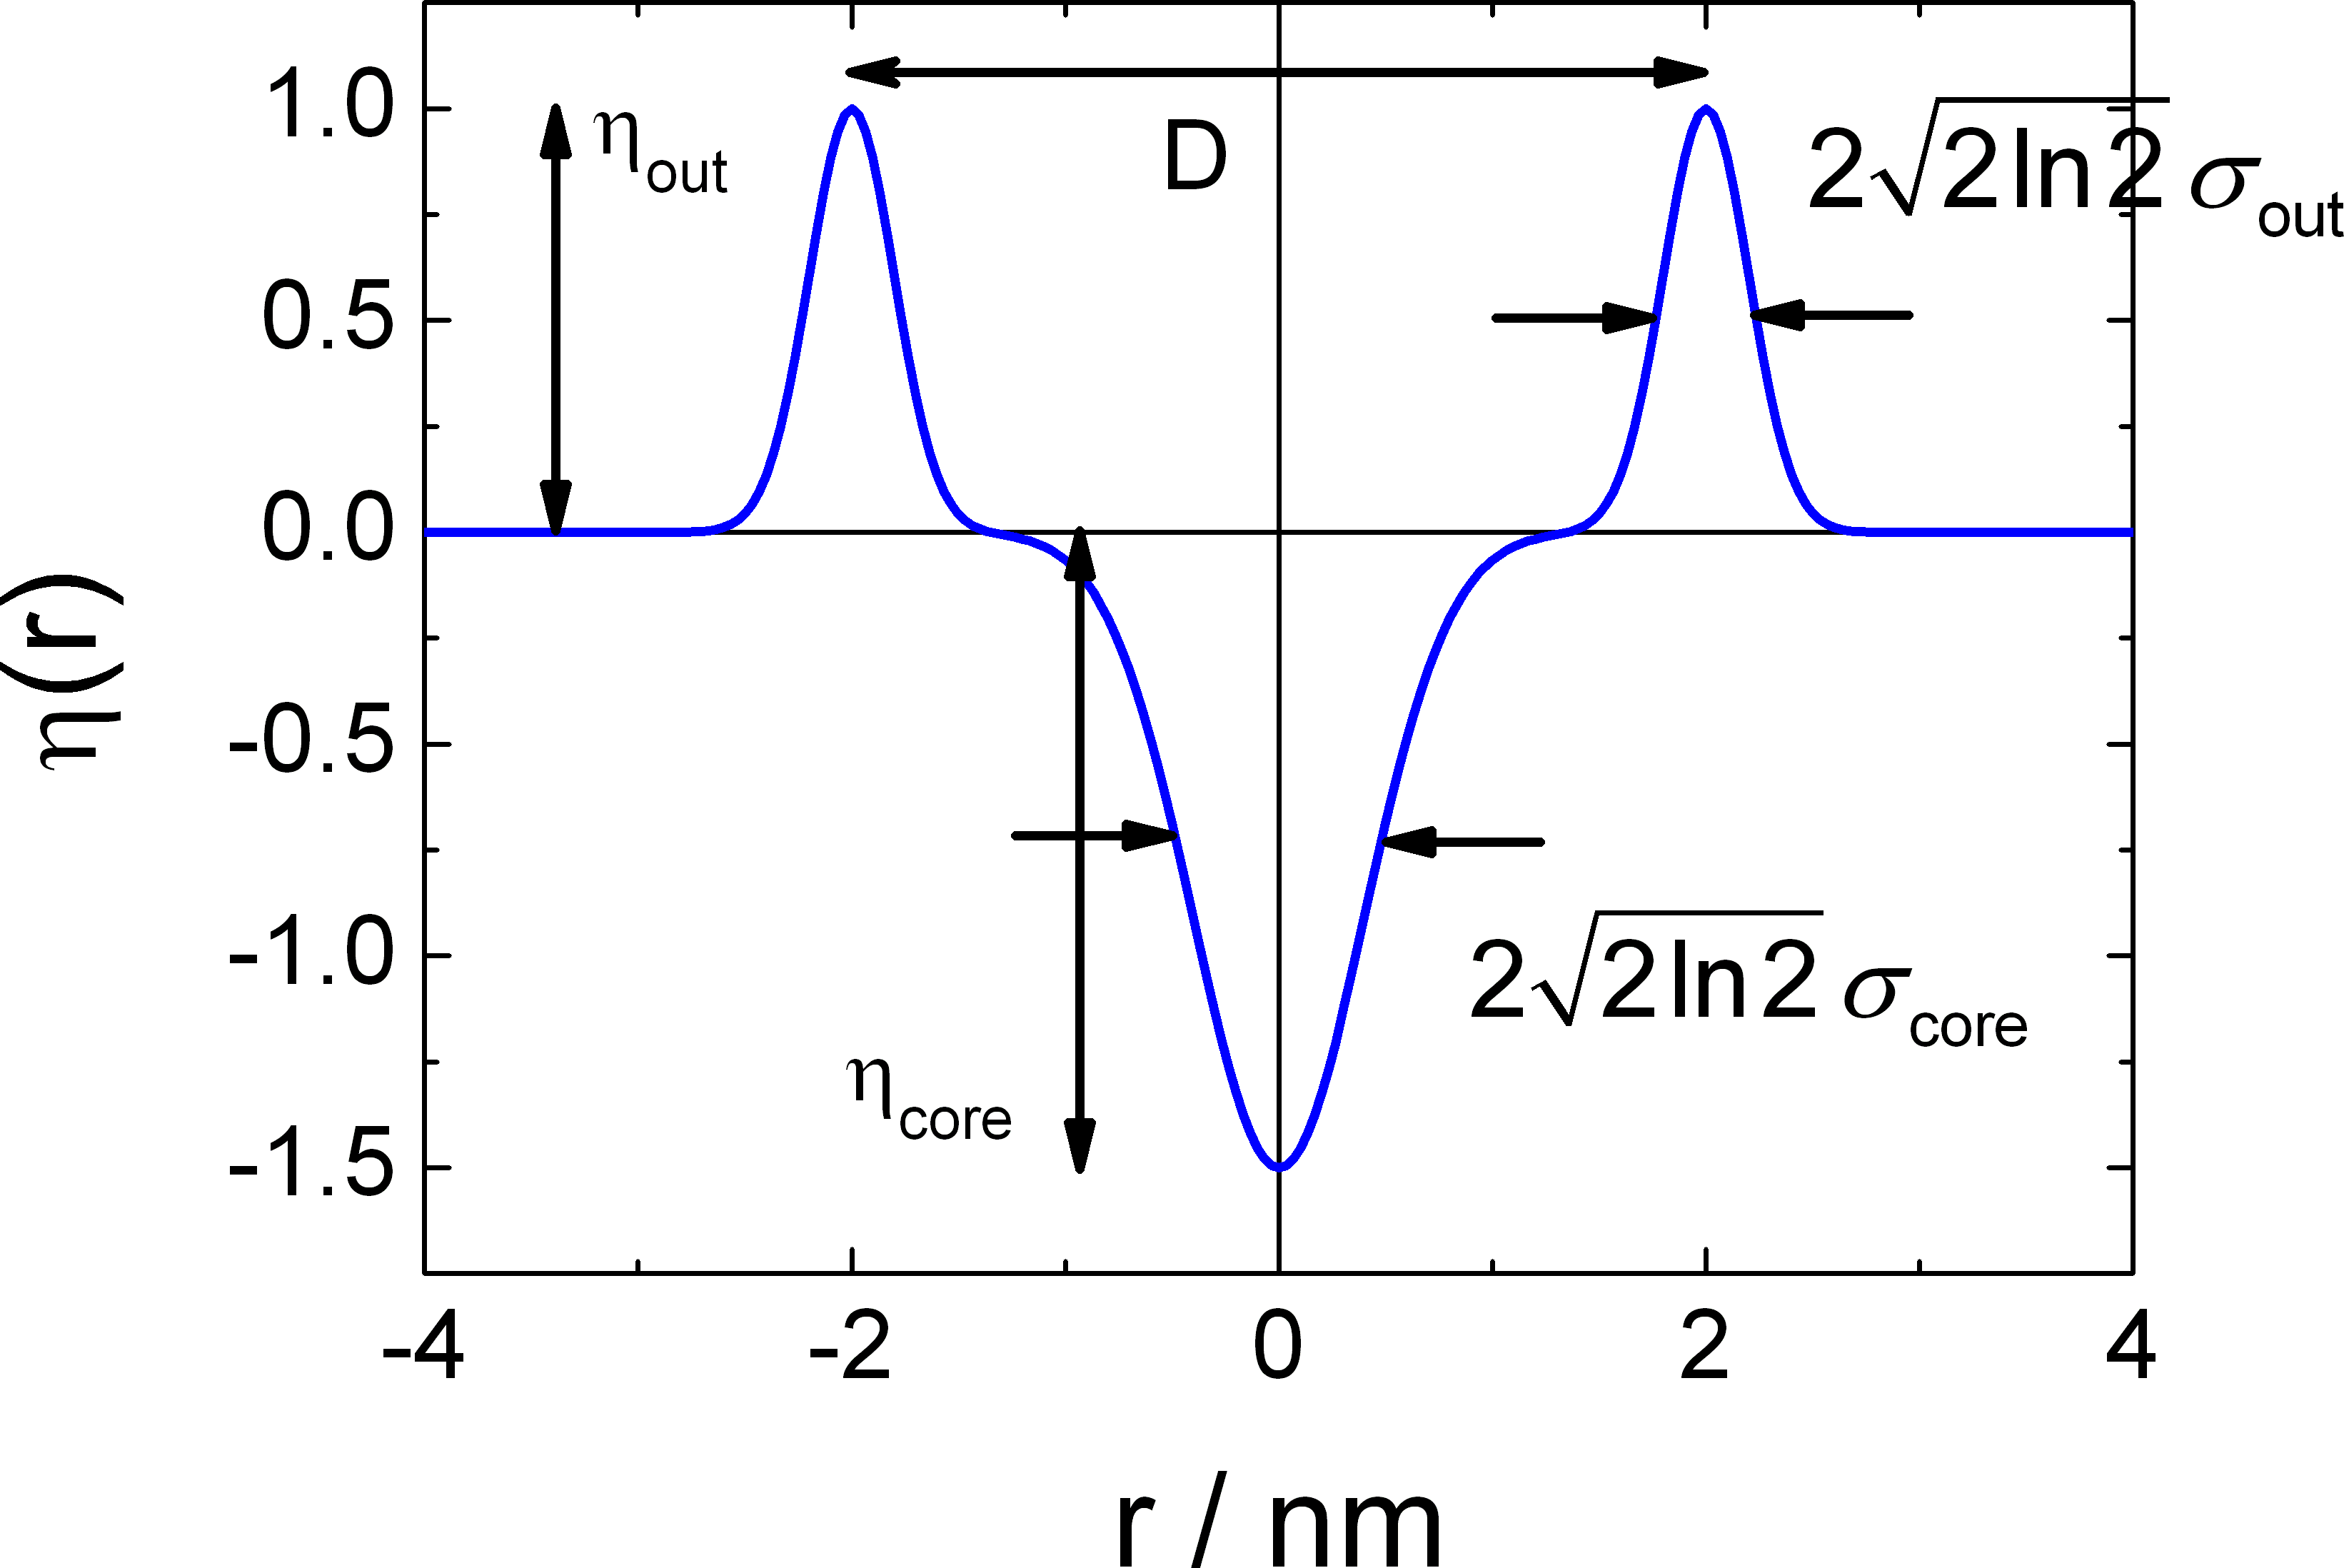
\includegraphics[width=0.8\textwidth,height=0.55\textwidth]{../images/form_factor/anisotropic/BiLayerGauss_Profile.png}
\end{center}
\caption{
The plot shows a model for the Gaussian description of the bilayer electron density profile according to
eq.\ \ref{eq:BiLayerGaussianProfile}.
The origin of the profile is set to the bilayer centre. The model encountering a single Gaussian for the head
group at $\pm t/2$. $\eta_\textrm{out}$ is the amplitude of the headgroup Gaussian and $\eta_\textrm{core}$ that of
the hydrocarbon chains with respect to the average electron density of water. The FWHM of the Gaussian profiles are
$2\sqrt{2\ln 2}\sigma_\textrm{out}$ and $2\sqrt{2\ln 2}\sigma_\textrm{core}$.}
\label{fig:bilayerprofile}
\end{figure}

This model for a bilayer is using a real-space representation of the electron density profile
using a Gaussian description \cite{Pabst2000,Pabst2003}. In comparison to other models it
is simpler and requiring the adjustment of only four parameters. The electron density profile
(Fig.\ \ref{fig:bilayerprofile}) is described by
\begin{align}
\begin{split}
\eta(r) &=  \eta_\textrm{out} \left[ \exp\left(-\frac{\left(r-\frac{t}{2}\right)^2}{2\sigma_\textrm{out}^2}\right) +
   \exp\left(-\frac{\left(r+\frac{t}{2}\right)^2}{2\sigma_\textrm{out}^2}\right) \right] \\
          &+ \eta_\textrm{core} \exp\left(-\frac{r^2}{2\sigma_\textrm{core}^2}\right)
          \label{eq:BiLayerGaussianProfile}
\end{split}
\end{align}
The scattering intensity of this cross section profile of a planar object can be calculated by eq.\ \ref{Pcs:planar}
and computes as
\begin{align}
   F_\text{out}\left(Q,D,\sigma_\textrm{out},\eta_\textrm{out}\right)  &= \sqrt{2\pi}\sigma_\textrm{out}  \eta_\textrm{out}  \exp\left(-\frac{1}{2}\left(Q\sigma_\textrm{out} \right)^2\right) \cos\left(Q\frac{t}{2}\right) \\
   F_\text{core}\left(Q,\sigma_\textrm{core},\eta_\textrm{core}\right) &= \sqrt{2\pi}\sigma_\textrm{core} \eta_\textrm{core} \exp\left(-\frac{1}{2}\left(Q\sigma_\textrm{core}\right)^2\right)
\end{align}
so that
\begin{align}
  P_\text{cs}\left(Q\right)   &=\left[F_\text{core}\left(Q,\sigma_\textrm{core}, \eta_\textrm{core}\right)
                                   +2 F_\text{out} \left(Q,D,\sigma_\textrm{out},\eta_\textrm{out} \right)\right]^2
  \label{eq:PcsBilayer}
\end{align}

\vspace{5mm}

\hspace{1pt}\\
\underline{Input parameters for \texttt{Pcs:BilayerGauss}:}
\begin{description}
    \item[\texttt{sigma\_core}] width $\sigma_\mathrm{out}$ of the central Gaussian profile
    \item[\texttt{eta\_core}] scattering length density contrast of the central Gaussian profile
    \item[\texttt{sigma\_out}] width $\sigma_\mathrm{out}$ of the two outer Gaussian profiles
    \item[\texttt{eta\_out}] scattering length density contrast of the two outer Gaussian profiles
    \item[\texttt{t}] distance between the centers of the outer Gaussian profiles
\end{description}

\noindent
\underline{Note}
\begin{itemize}
  \item This form factor is supposed to be combined with a shape factor for
local planar objects which are implemented as structure  plugins
under "\texttt{[by plugin|thin obj.|P'(Q): local planar
obj.]}".
\end{itemize}

\begin{figure}[htb]
\begin{center}
\subfigure[Plot of the cross section form factor $P_\text{cs}$ in combination with a structure factor "\texttt{P'(Q): Thin Disc}"
as the shape factor $P'(Q)$.]{
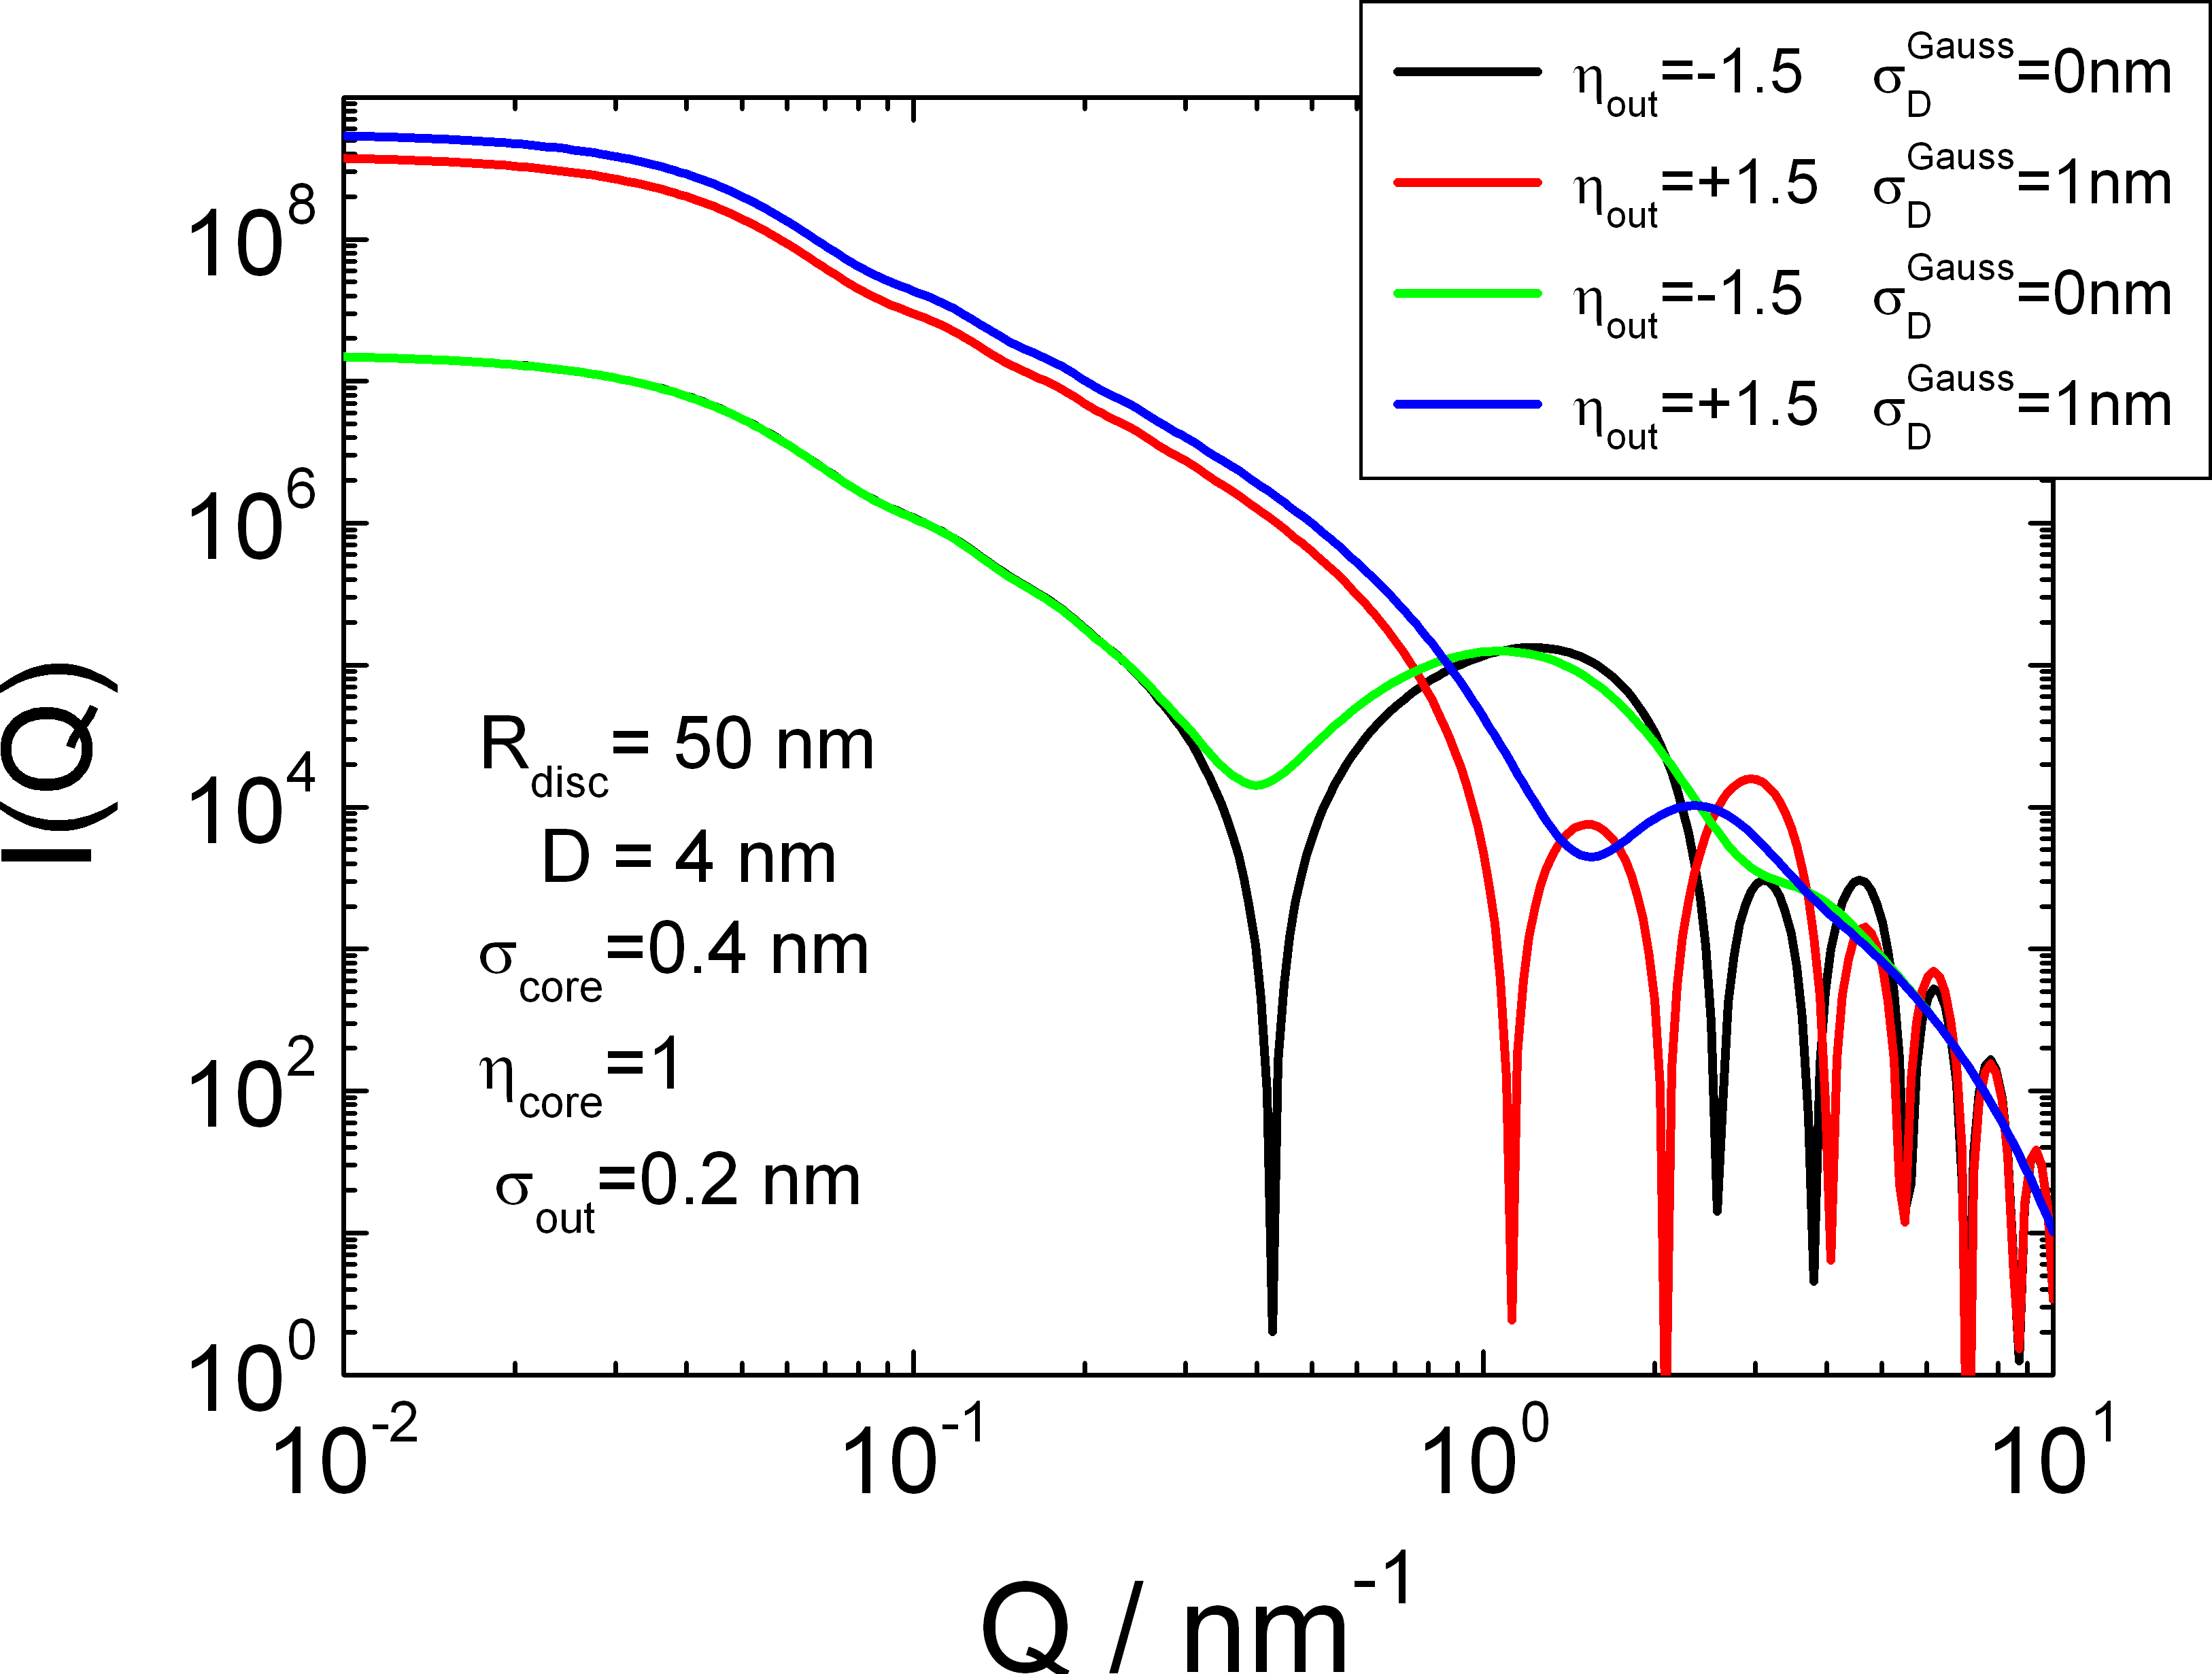
\includegraphics[width=0.48\textwidth,height=0.35\textwidth]{../images/form_factor/anisotropic/BiLayerGauss_IQa.png}}
\hfill
\subfigure[Plot of the cross section form factor $P_\text{cs}$ only according to eq.\ \ref{eq:PcsBilayer}.
The parameters for the profile are the same than in Fig.\ \ref{fig:BiLayerGaussianProfileIQ}a]{
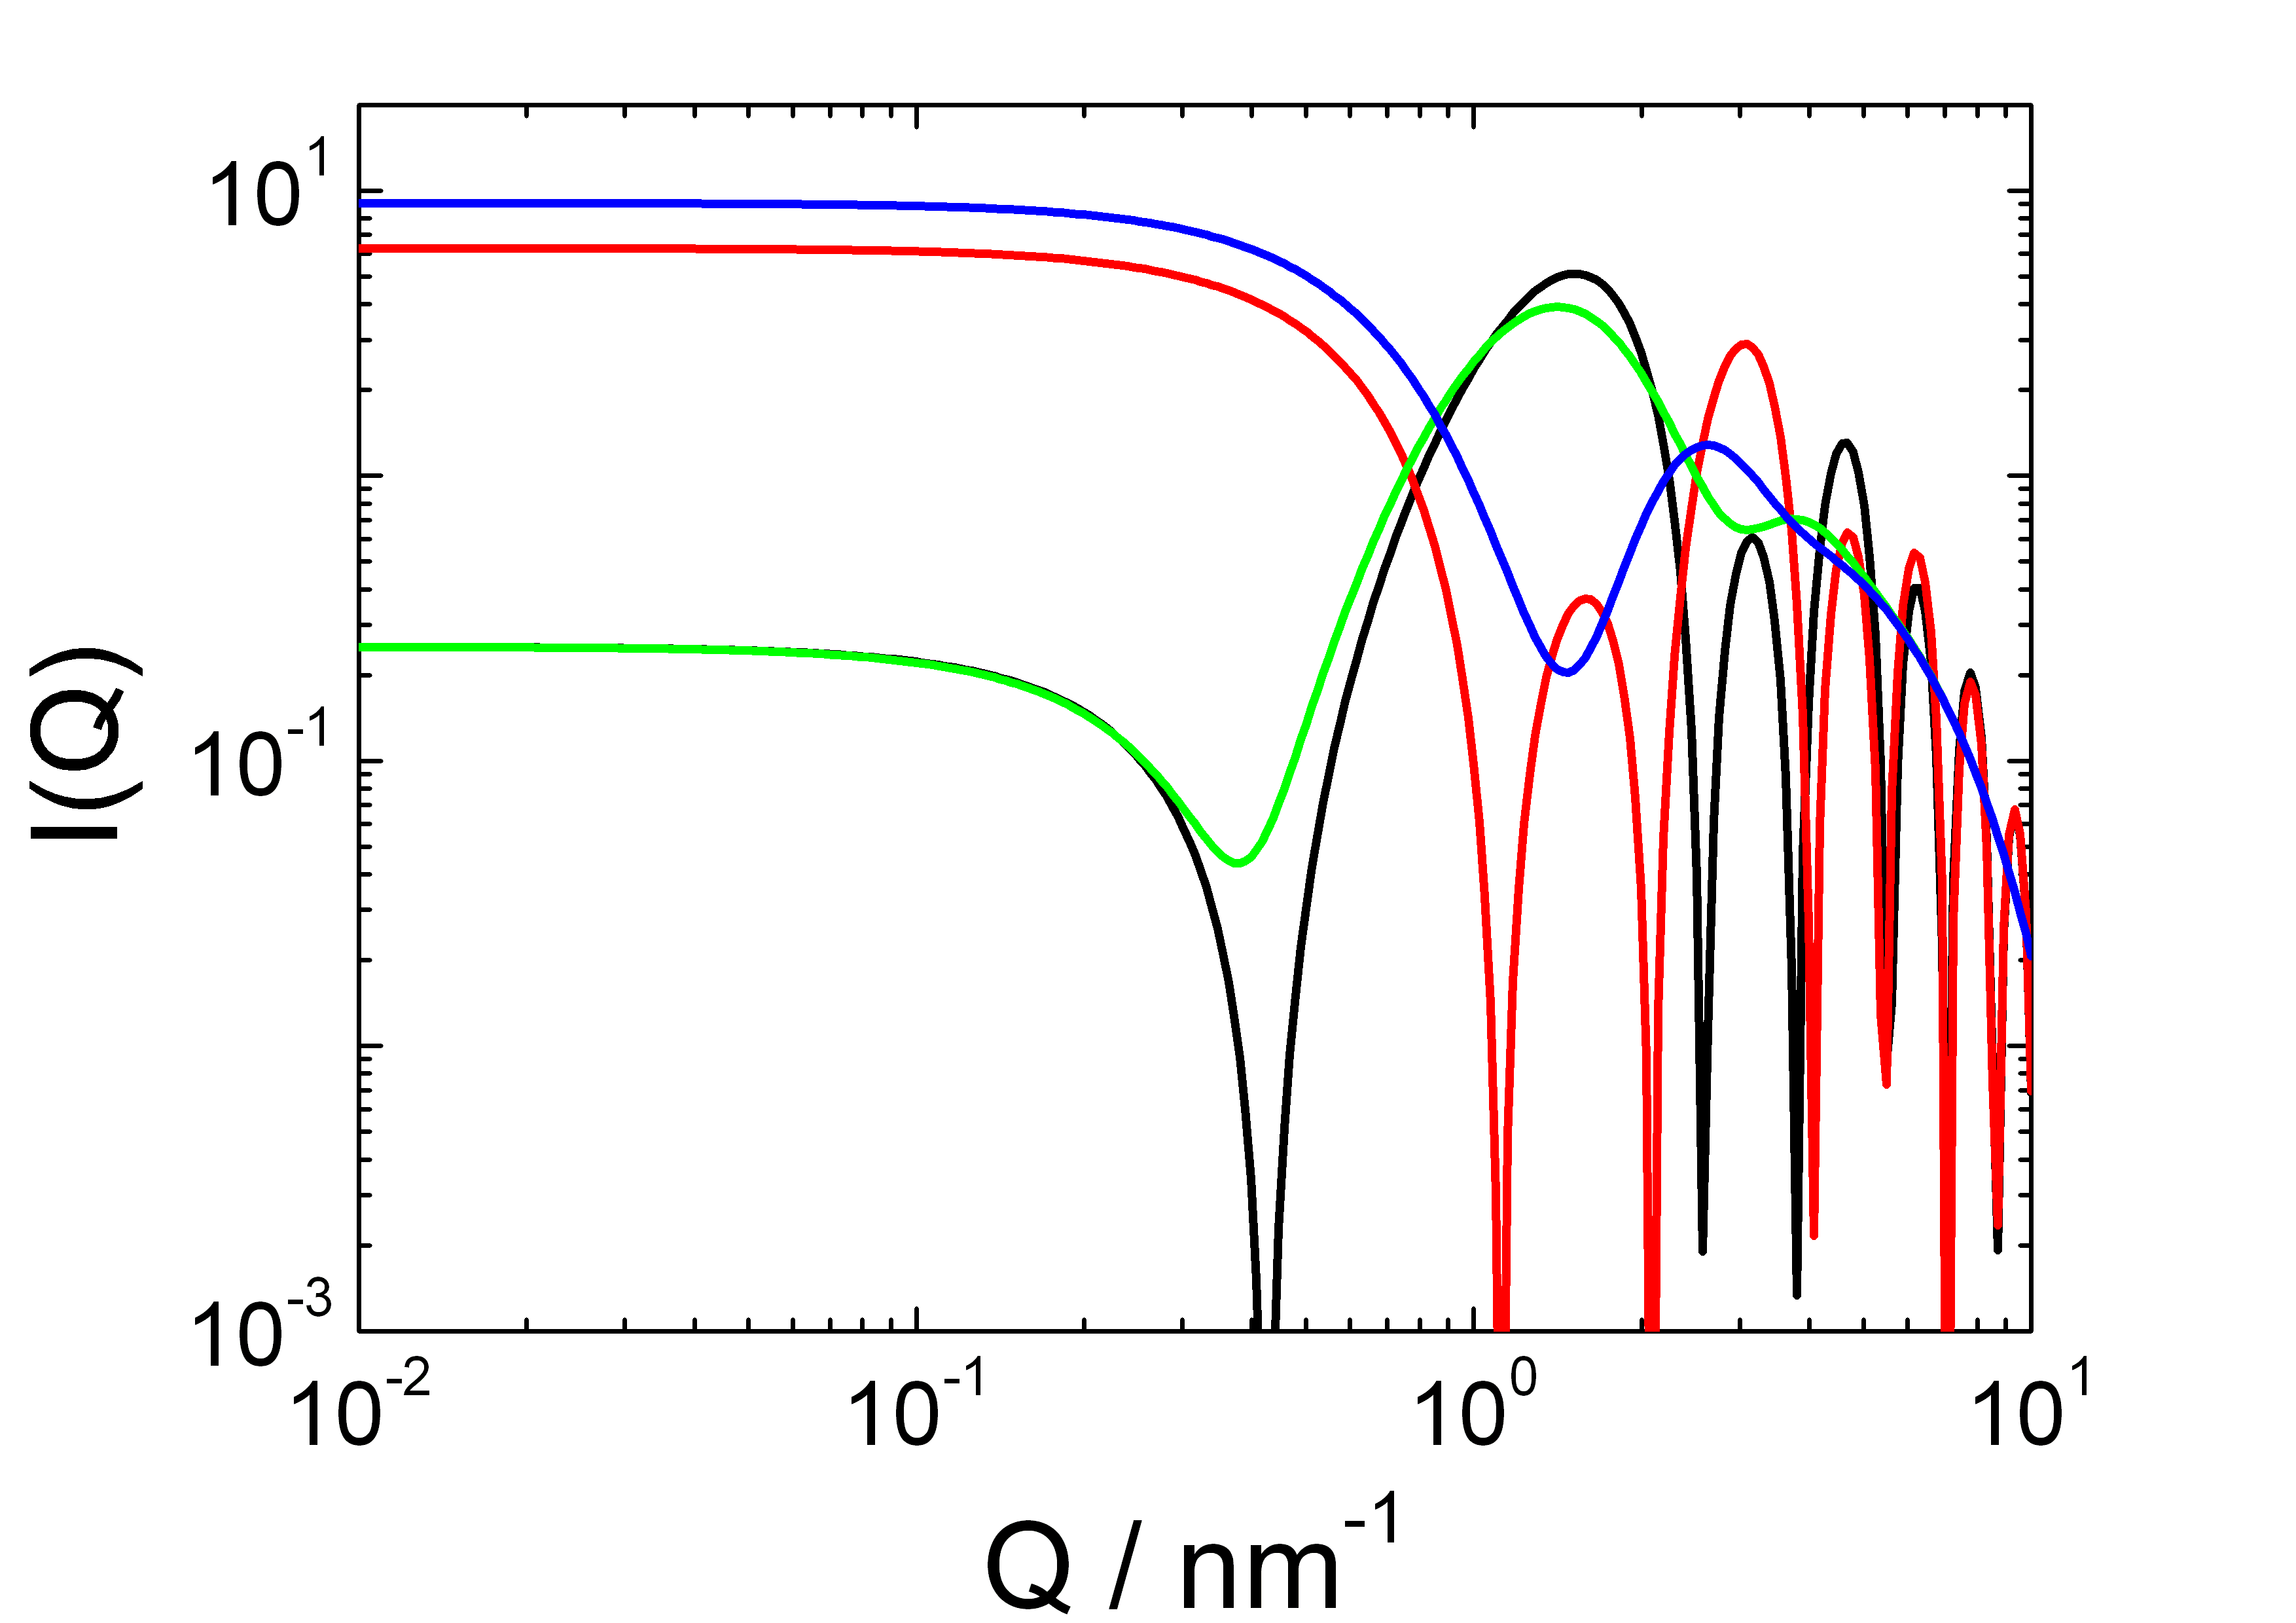
\includegraphics[width=0.48\textwidth,height=0.35\textwidth]{../images/form_factor/anisotropic/BiLayerGauss_IQb.png}}
\end{center}
\caption{Scattering curve for the cross-section form factor "\texttt{Pcs:BilayerGaussian}". For some of the curves a distance distribution of
the heads groups are assumed being Gaussian (see eq.\ \ref{eq:GaussDistribution}), i.e. calculating
$\int_0^\infty \mathrm{Gauss}(D,1,\sigma_D^\textrm{Gauss},D_0) P_\text{cs}\left(Q,D\right)\, \mathrm{d}D$.}
\label{fig:BiLayerGaussianProfileIQ}
\end{figure}


%
%\clearpage
%\subsubsection{Pcs(Q) for local planar objects with Gaussian chains attached to the  surface} ~\\
%\label{plugin:Pcs:GaussianChains}
%
%\begin{figure}[htb]
%\begin{center}
%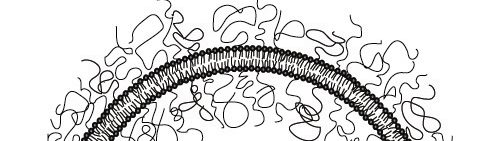
\includegraphics[width=0.962\textwidth,height=0.282\textwidth]{../images/form_factor/anisotropic/Plate+Chains(RW).png}
%\end{center}
%\caption{Sketch of a lipid bilayer with PEG molecules attached to them, which would be an example for local planar
%and objects with homogeneous core and Gaussian chains attached to the surface.}
%\label{fig:Plate+Chains(RW)}
%\end{figure}
%
%This cross-section form factor belongs to a whole class of form factors developed from
%Pedersen, Gerstenberg, and Svaneborg
%\cite{PedersenJApplCryst2000,PedersenGerstenberg96,SvaneborgPedersen2002,Richter1997}
%for self assembled block copolymers forming micelles of different shapes.
%They have assumed that one unit is forming the core of the
%micelles and the other the corona. The core is assumed to have a
%homogeneous scattering length density, but may contain some amount
%of solvent whereas the soluble blocks form a diffuse corona surrounding the core.
%
%The cross-section form factor of a micelle contains four different terms \cite{Pedersen2002}
%\begin{align}
%\begin{split}
%P_\text{cs}(Q)
% &=  \Bigg( r_\textrm{core}^2\,\left(\frac{\sin(QL/2)}{QL/2}\right)^2 + r_\textrm{brush} N_\text{agg} P_\text{brush}(Q)  \\
% & + N_\text{agg}(N_\text{agg}-1)r_\text{brush}^2\,S_\textrm{bb}(Q) + 2N_\text{agg} r_\text{core}r_\text{brush}\,S_\text{bc}(Q)\Bigg)
%\end{split}
%\end{align}
%where $N_\text{agg}$ is the total aggregation number of polymers on the surface, and
%$r_\text{brush}=V_\text{brush}(\eta_\text{brush}-\eta_\text{solv})$
%the excess scattering length of a single polymer chain in the corona
%and $r_\text{core}=V_\text{core}(\eta_\text{core}-\eta_\text{solv})$
%the total  excess scattering length of the core, respectively.
%$V_\text{brush}$ is the volume of a a single polymer chain in the corona
%and $V_\text{core}$ the total volume of the core. $\eta_\text{brush}$ and $\eta_\text{core}$ are the corresponding
%scattering length densities and $\eta_\text{solv}$ is the scattering length
%density of the surrounding solvent.
%
%The functions $P_\text{core}(Q)$, $P_\text{brush}(Q)$,
%$S_\text{bc}(Q)$, and $S_\text{bb}(Q)$ are all 1 for $q=0$.
%They are defined as
%
%\noindent
%\textbf{Input parameters for \texttt{Pcs:Plate+Chains(RW)}:}
%\begin{description}
%    \item[\texttt{L\_core}] thickness of the core of the planar layer $L_\textrm{core}$
%    \item[\texttt{n\_agg}] specific aggregation number $n_\textrm{agg}$ in units of number of chains per surface area
%    \item[\texttt{V\_brush}]  molecular volume of single chain in corona $V_\textrm{brush}$ in nm$^3$ for $Q$ in nm$^{-1}$
%                              or in \AA$^3$ for $Q$ in \AA$^{-1}$
%    \item[\texttt{eta\_core}] scattering length density of the core $\eta_\textrm{core}$
%    \item[\texttt{eta\_brush}] scattering length density of a Gaussian chain in corona $\eta_\textrm{brush}$
%    \item[\texttt{eta\_solv}] scattering length density of solvent $\eta_\textrm{solv}$
%    \item[\texttt{xsolv\_core}] amount of solvent in core $X_\textrm{xsolc,core}$
%    \item[\texttt{Rg}] gyration radius $R_G$ of polymer chains in the corona
%    \item[\texttt{d}] Value $d$ should be around 1.
%                      Non-penetration of the chains into the core is mimicked by $d\simeq 1$ for $L_\textrm{core} \gg R_G$
%\end{description}
%
%\noindent
%\underline{Note}
%\begin{itemize}
%  \item This form factor is supposed to be combined with a shape factor for
%local planar objects which are implemented as structure  plugins
%under "\texttt{by plugin|anisotropic obj.|P'(Q): local planar
%obj.}".
%\end{itemize}
%
%\begin{figure}[htb]
%\begin{center}
%\subfigure[Plot of the cross section form factor $P_\text{cs}$ only according to eq.\ \ref{eq:PcsBilayer}.]{
%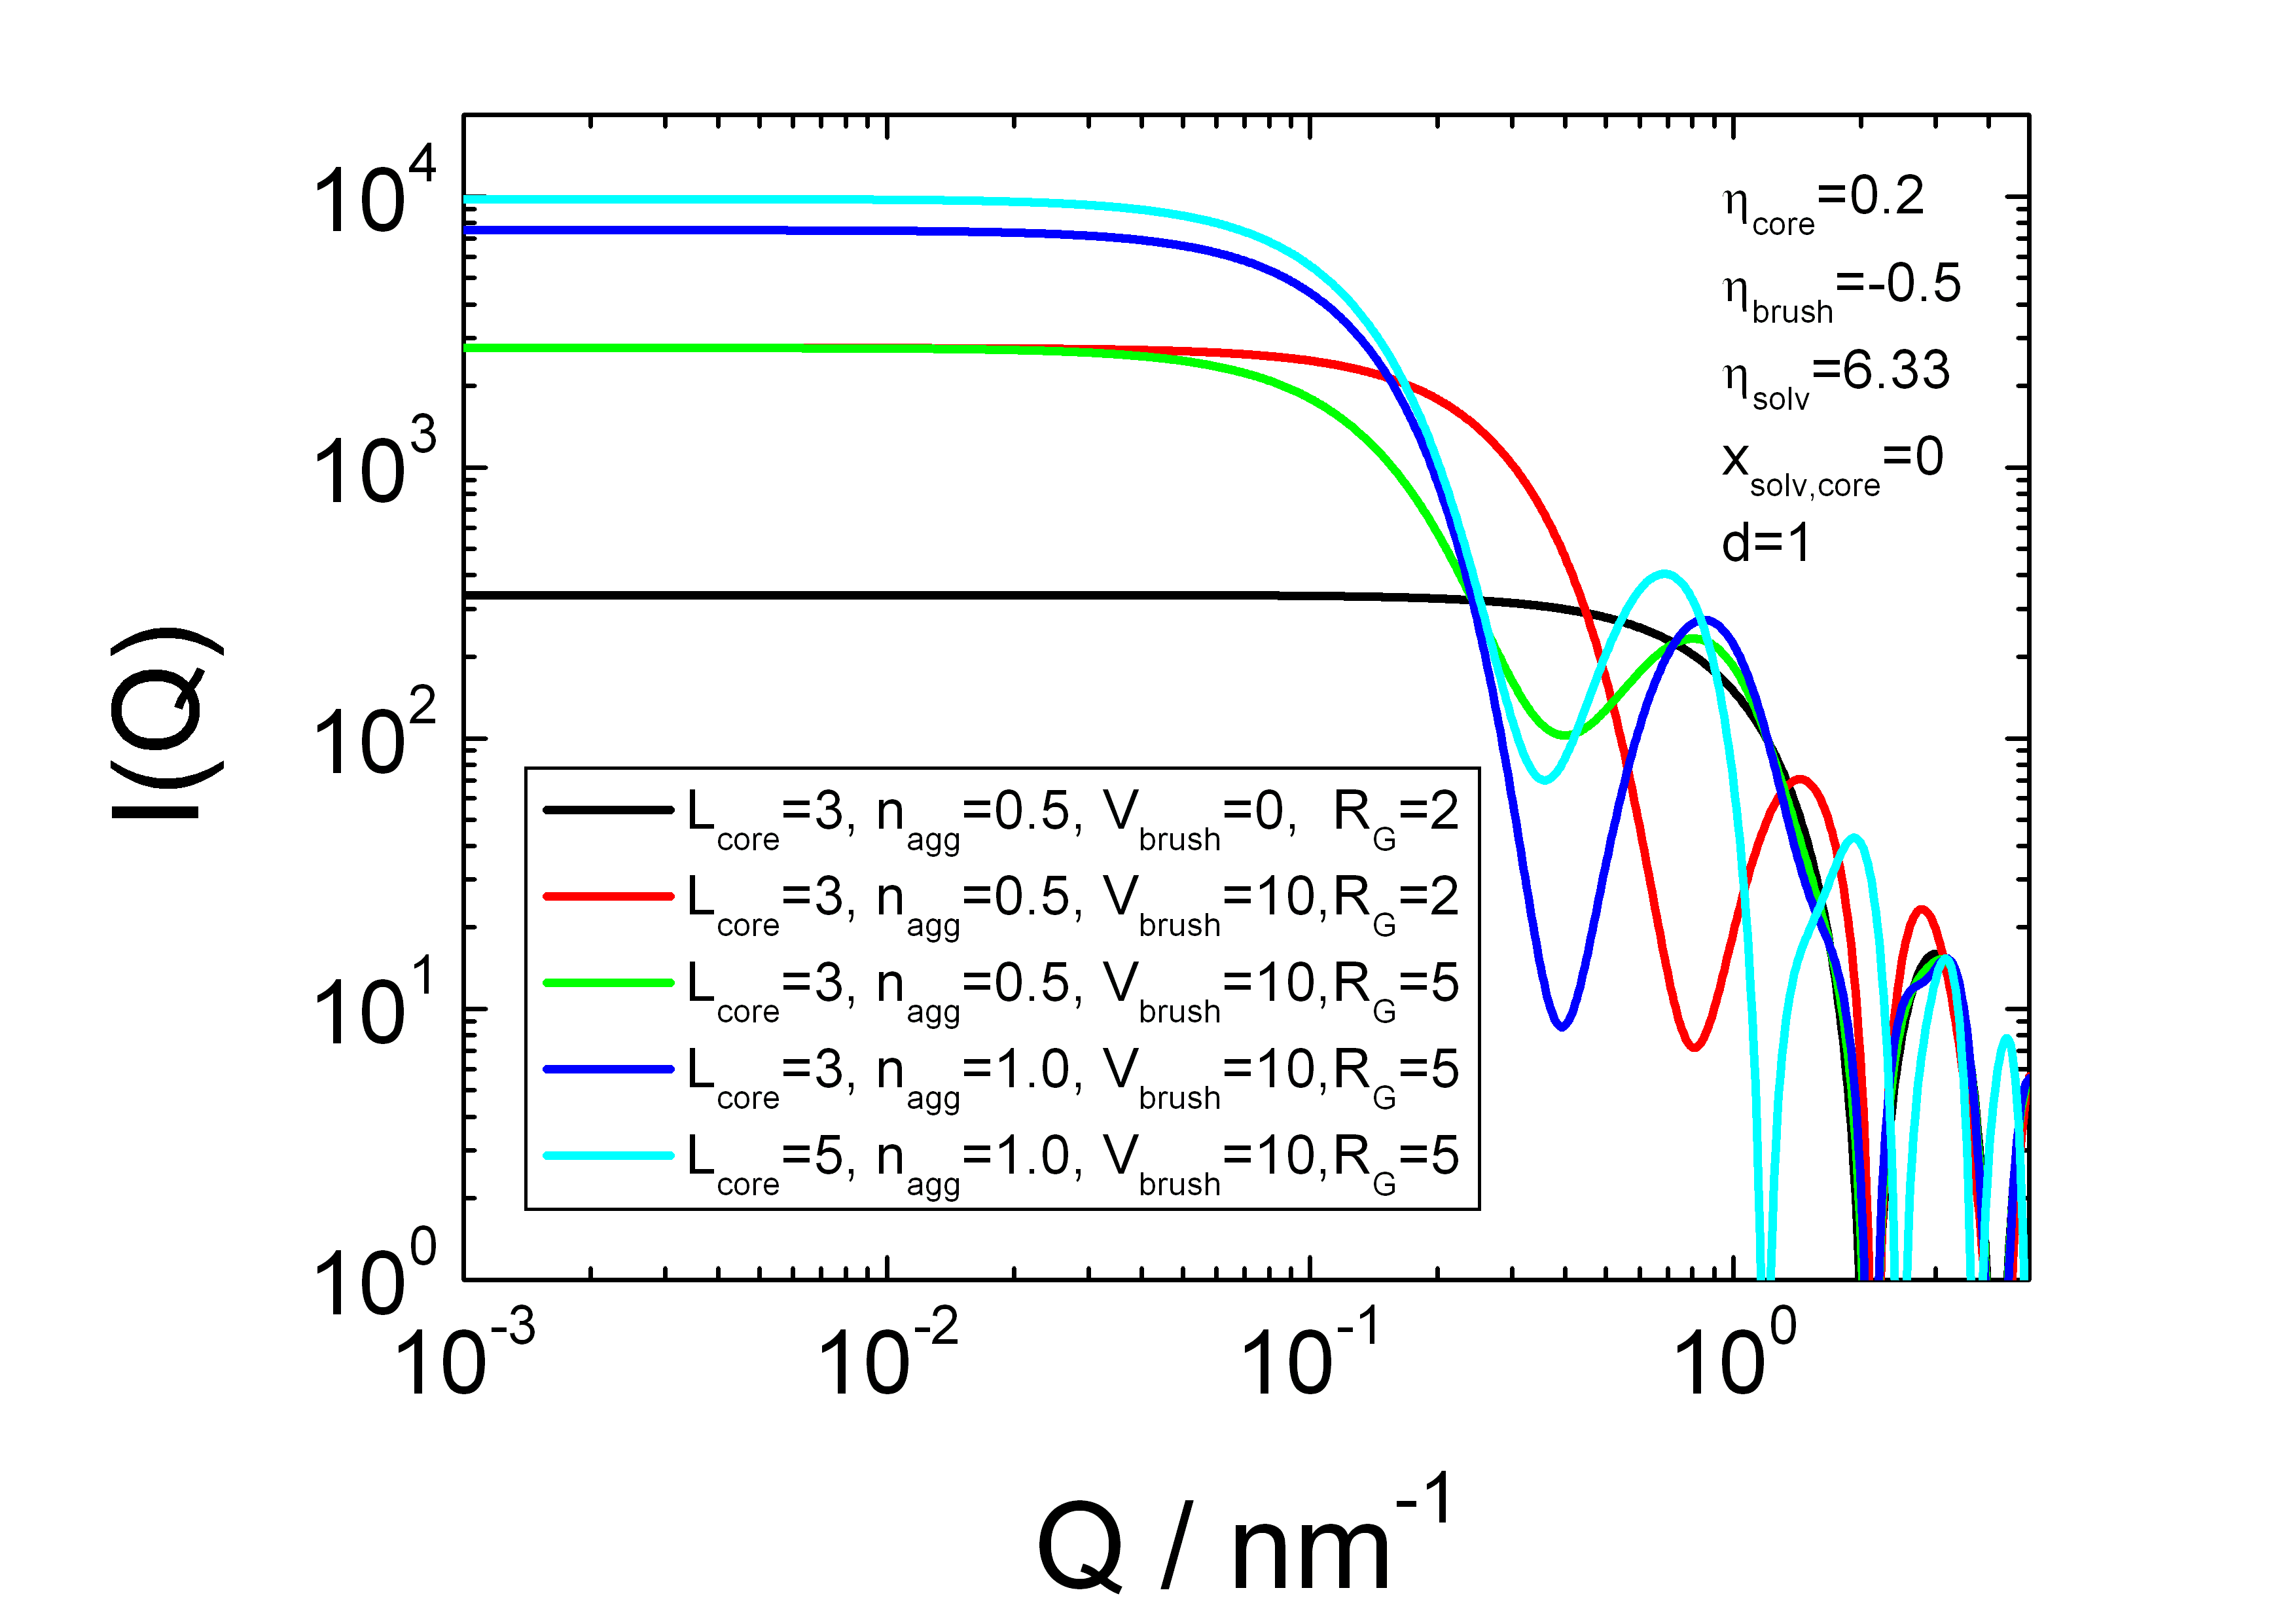
\includegraphics[width=0.48\textwidth,height=0.35\textwidth]{../images/form_factor/anisotropic/Pcs_Plate_Chains_RW_IQa.png}}
%\hfill
%\subfigure[Plot of the cross section form factor $P_\text{cs}$ in combination with a structure factor "\texttt{P'(Q): Thin Spherical Shell}"
%as the shape factor $P'(Q)$. The parameters for the profile are the same than in Fig.\ \ref{fig:Pcs_Plate_Chains_RW_IQ}a]{
%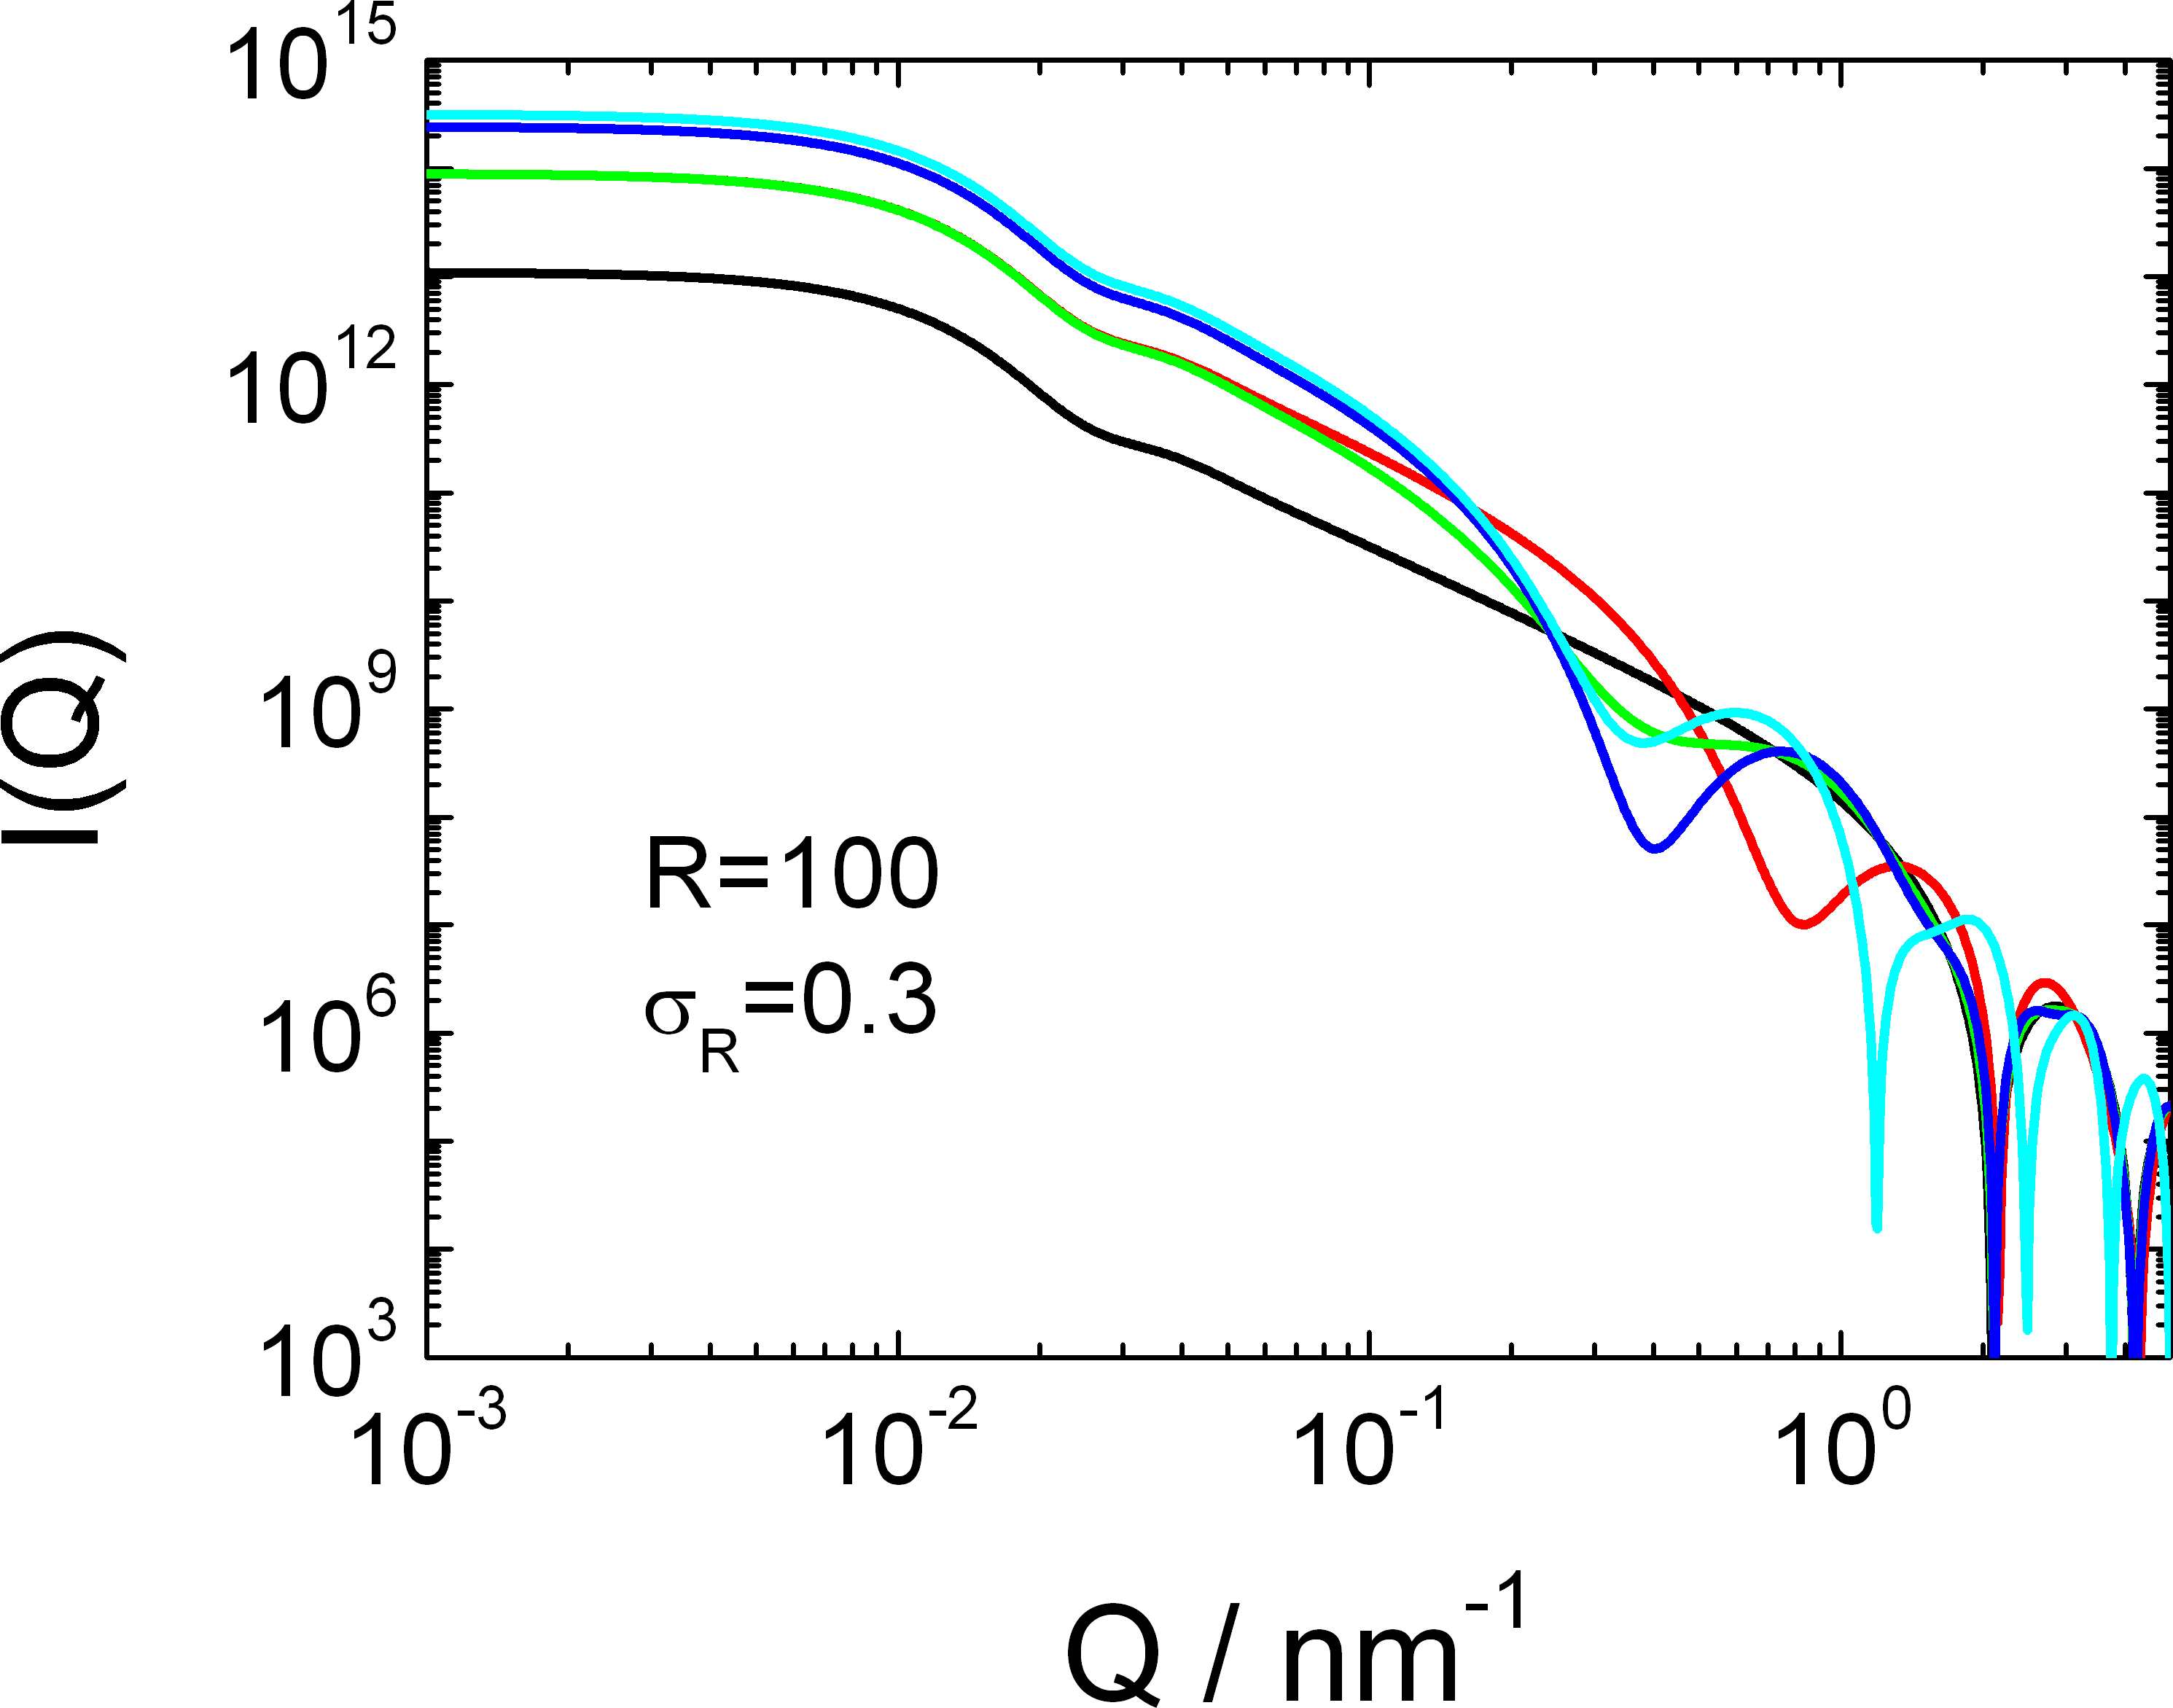
\includegraphics[width=0.48\textwidth,height=0.35\textwidth]{../images/form_factor/anisotropic/Pcs_Plate_Chains_RW_IQb.png}}
%\end{center}
%\caption{Scattering curves for the cross-section form factor "\texttt{Pcs:Plate+Chains(RW)}".}
%\label{fig:Pcs_Plate_Chains_RW_IQ}
%\end{figure}

\clearpage
\subsection{Pcs(Q) for cylindrical obj.} ~\\
\label{plugin:Pcs4cylindrical}

The cross-section form factors with cylindrical geometry are valid
when the cross-section dimension is much smaller than the segment length
or Kuhn length of the local cylindrical structure.

\begin{figure}[htb]
  % Requires \usepackage{graphicx}
  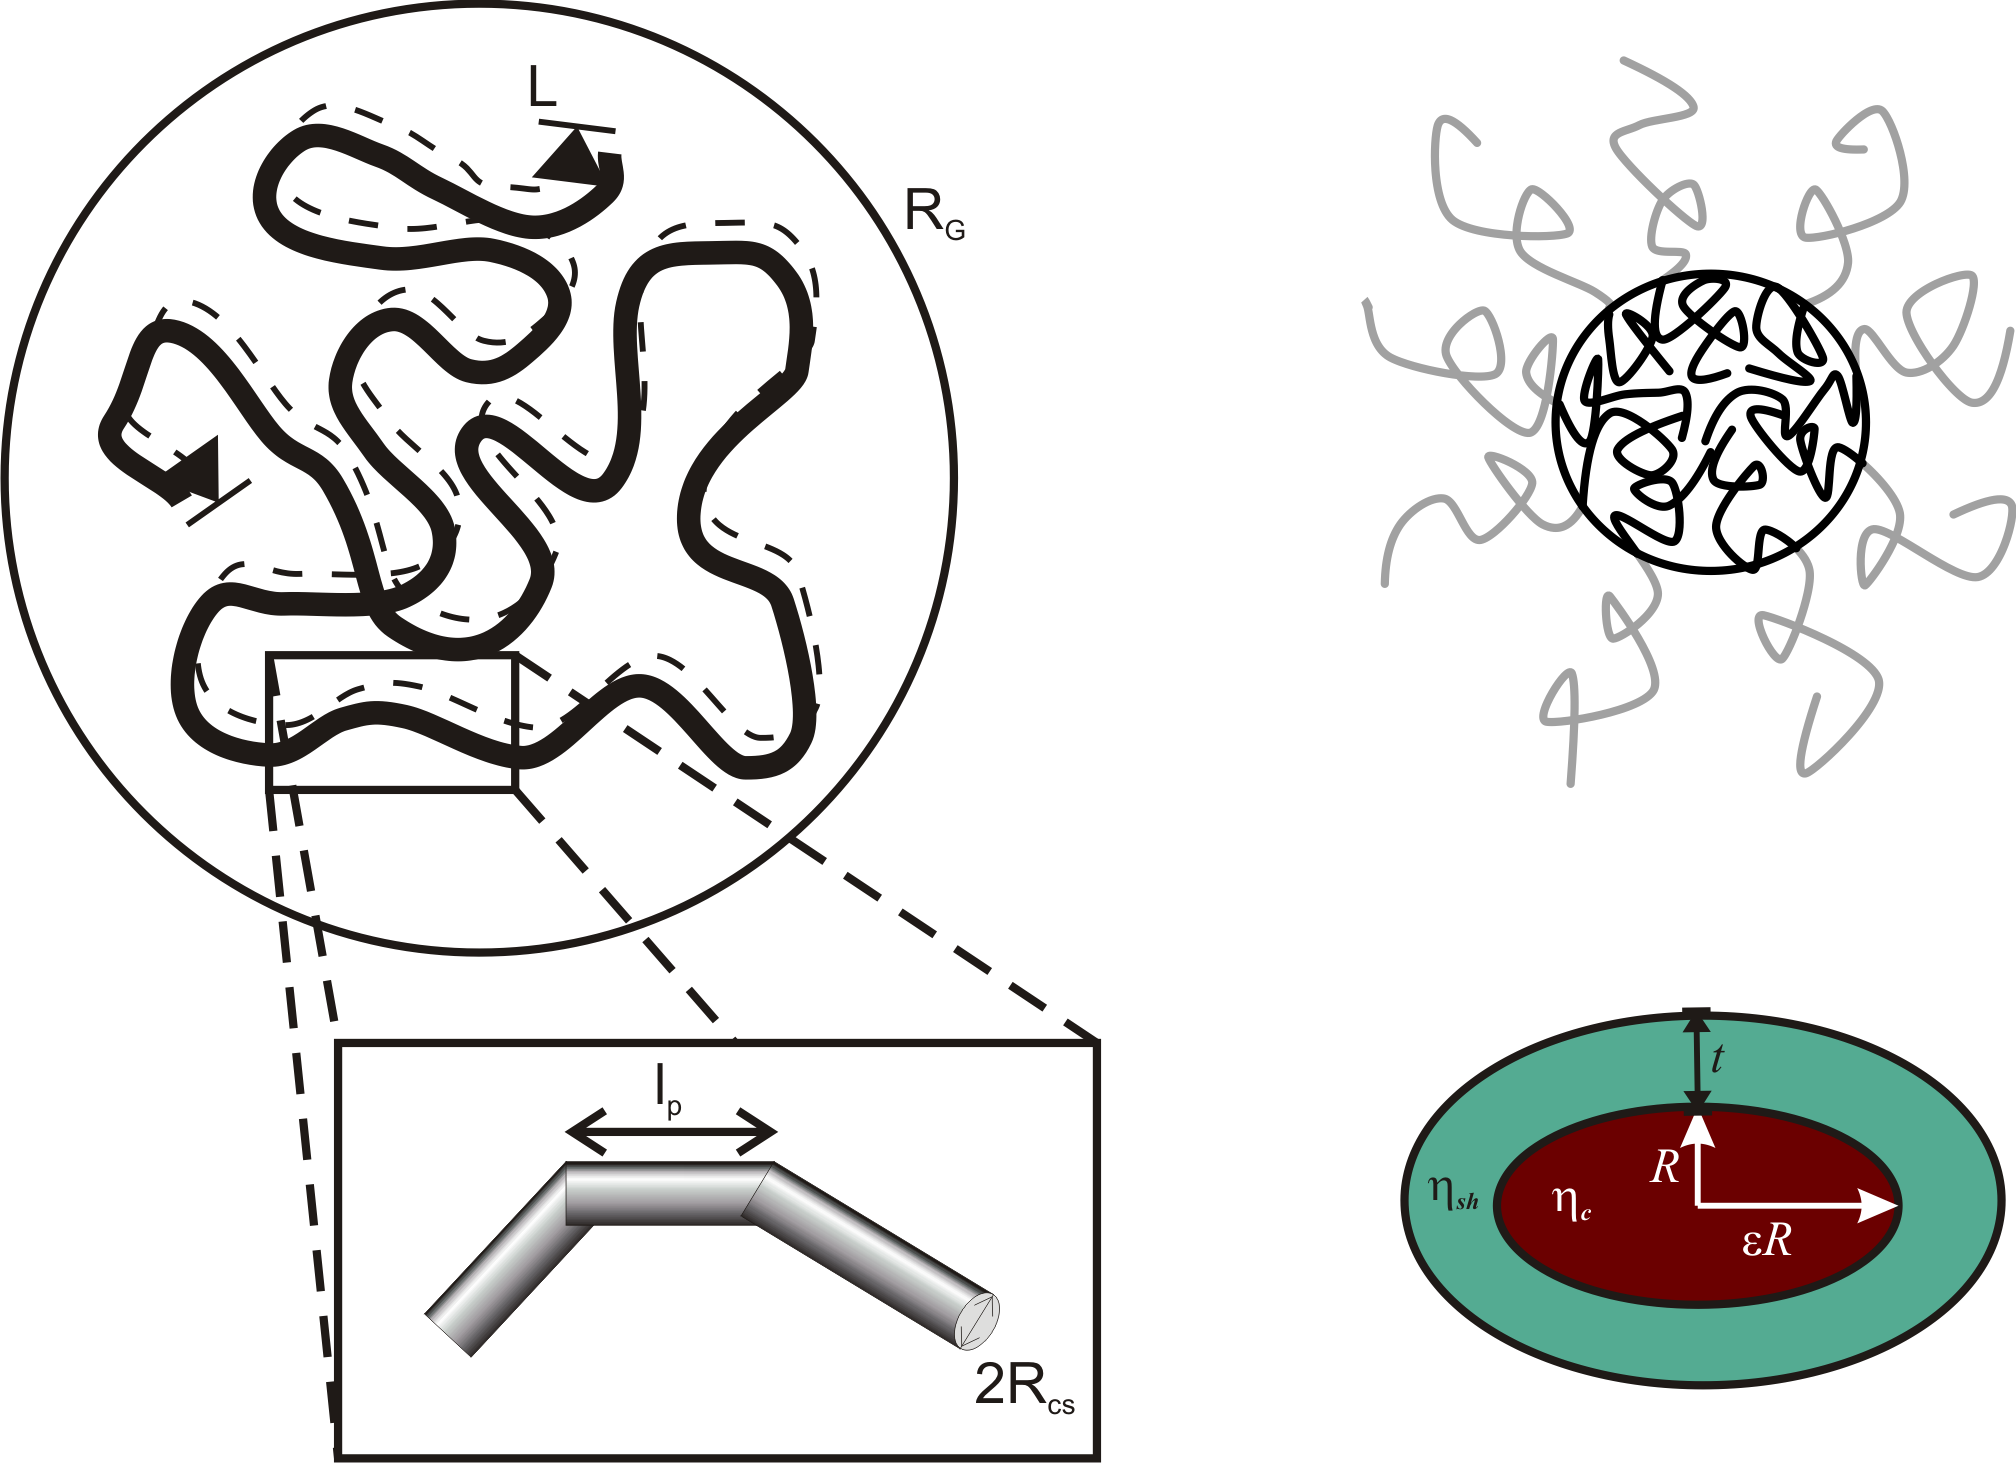
\includegraphics[width=0.85\textwidth]{../images/form_factor/anisotropic/SketchdiffXSWorm.png}\\
  \caption{Sketch of wormlike structures which represent local cylindrical structures. The cross-section $2R_\text{cs}$
  is much smaller than the Kuhn length $l_p$, which is a typical length scale where a freely jointed chain can randomly orient
  in any direction without the influence of any forces, independent of the directions taken by other segments.
  For the cross-section term several profiles have been implemented, like homogeneous round profile or elliptical shell profile}\label{fig:WormSketchdiffXS}
\end{figure}


\clearpage
\subsubsection{Pcs(Q) for homogeneous cross-section of a cylinder} ~\\
\label{plugin:Pcs:homogeneousXS_cyl}


This cross-section form factor describes the scattering of circular and homogeneous cross section.
The cross-section radius $R$ can have a distribution described by a log-normal distribution according
to eq.\ \ref{eq:LogNormal}.

\begin{align}
P_\text{cs}(Q,\sigma_{R},R) = \int_0^\infty \textrm{LogNorm}(x,1,\sigma_{R},1,R) \left( \left(\eta_\textrm{core}-\eta_\textrm{solv}\right) \pi x^2 \frac{2 \mathrm{J}_1(Qx)}{Qx} \right)^2 \, \textrm{d}x
\end{align}

\vspace{5mm}

\hspace{1pt}\\
\underline{Input parameters for \texttt{Pcs:homogeneousCyl}:}
\begin{description}
    \item[\texttt{R}] most probable radius $R$
    \item[\texttt{sigm\_R}] width $\sigma_R$ of radius distribution (LogNorm)
    \item[\texttt{dummy}] not used
    \item[\texttt{dummy}] not used
    \item[\texttt{dummy}] not used
    \item[\texttt{dummy}] not used
    \item[\texttt{dummy}] not used
    \item[\texttt{eta\_core}] scattering length density of the core $\eta_\textrm{core}$
    \item[\texttt{dummy}] not used
    \item[\texttt{eta\_solv}] scattering length density of the solvent $\eta_\textrm{solv}$
\end{description}

\noindent
\underline{Note}
\begin{itemize}
  \item This form factor is supposed to be combined with a shape factor for
local cylindrical objects which are implemented as structure  plugins
under "\texttt{[by plugin|thin obj.|P'(Q): local cylindrical obj.]}".
\item As the form factor already have the width distribution included one normally uses in \SASfit as a size distribution
the \texttt{Delta}-distribution.
\end{itemize}

\begin{figure}[htb]
\begin{center}
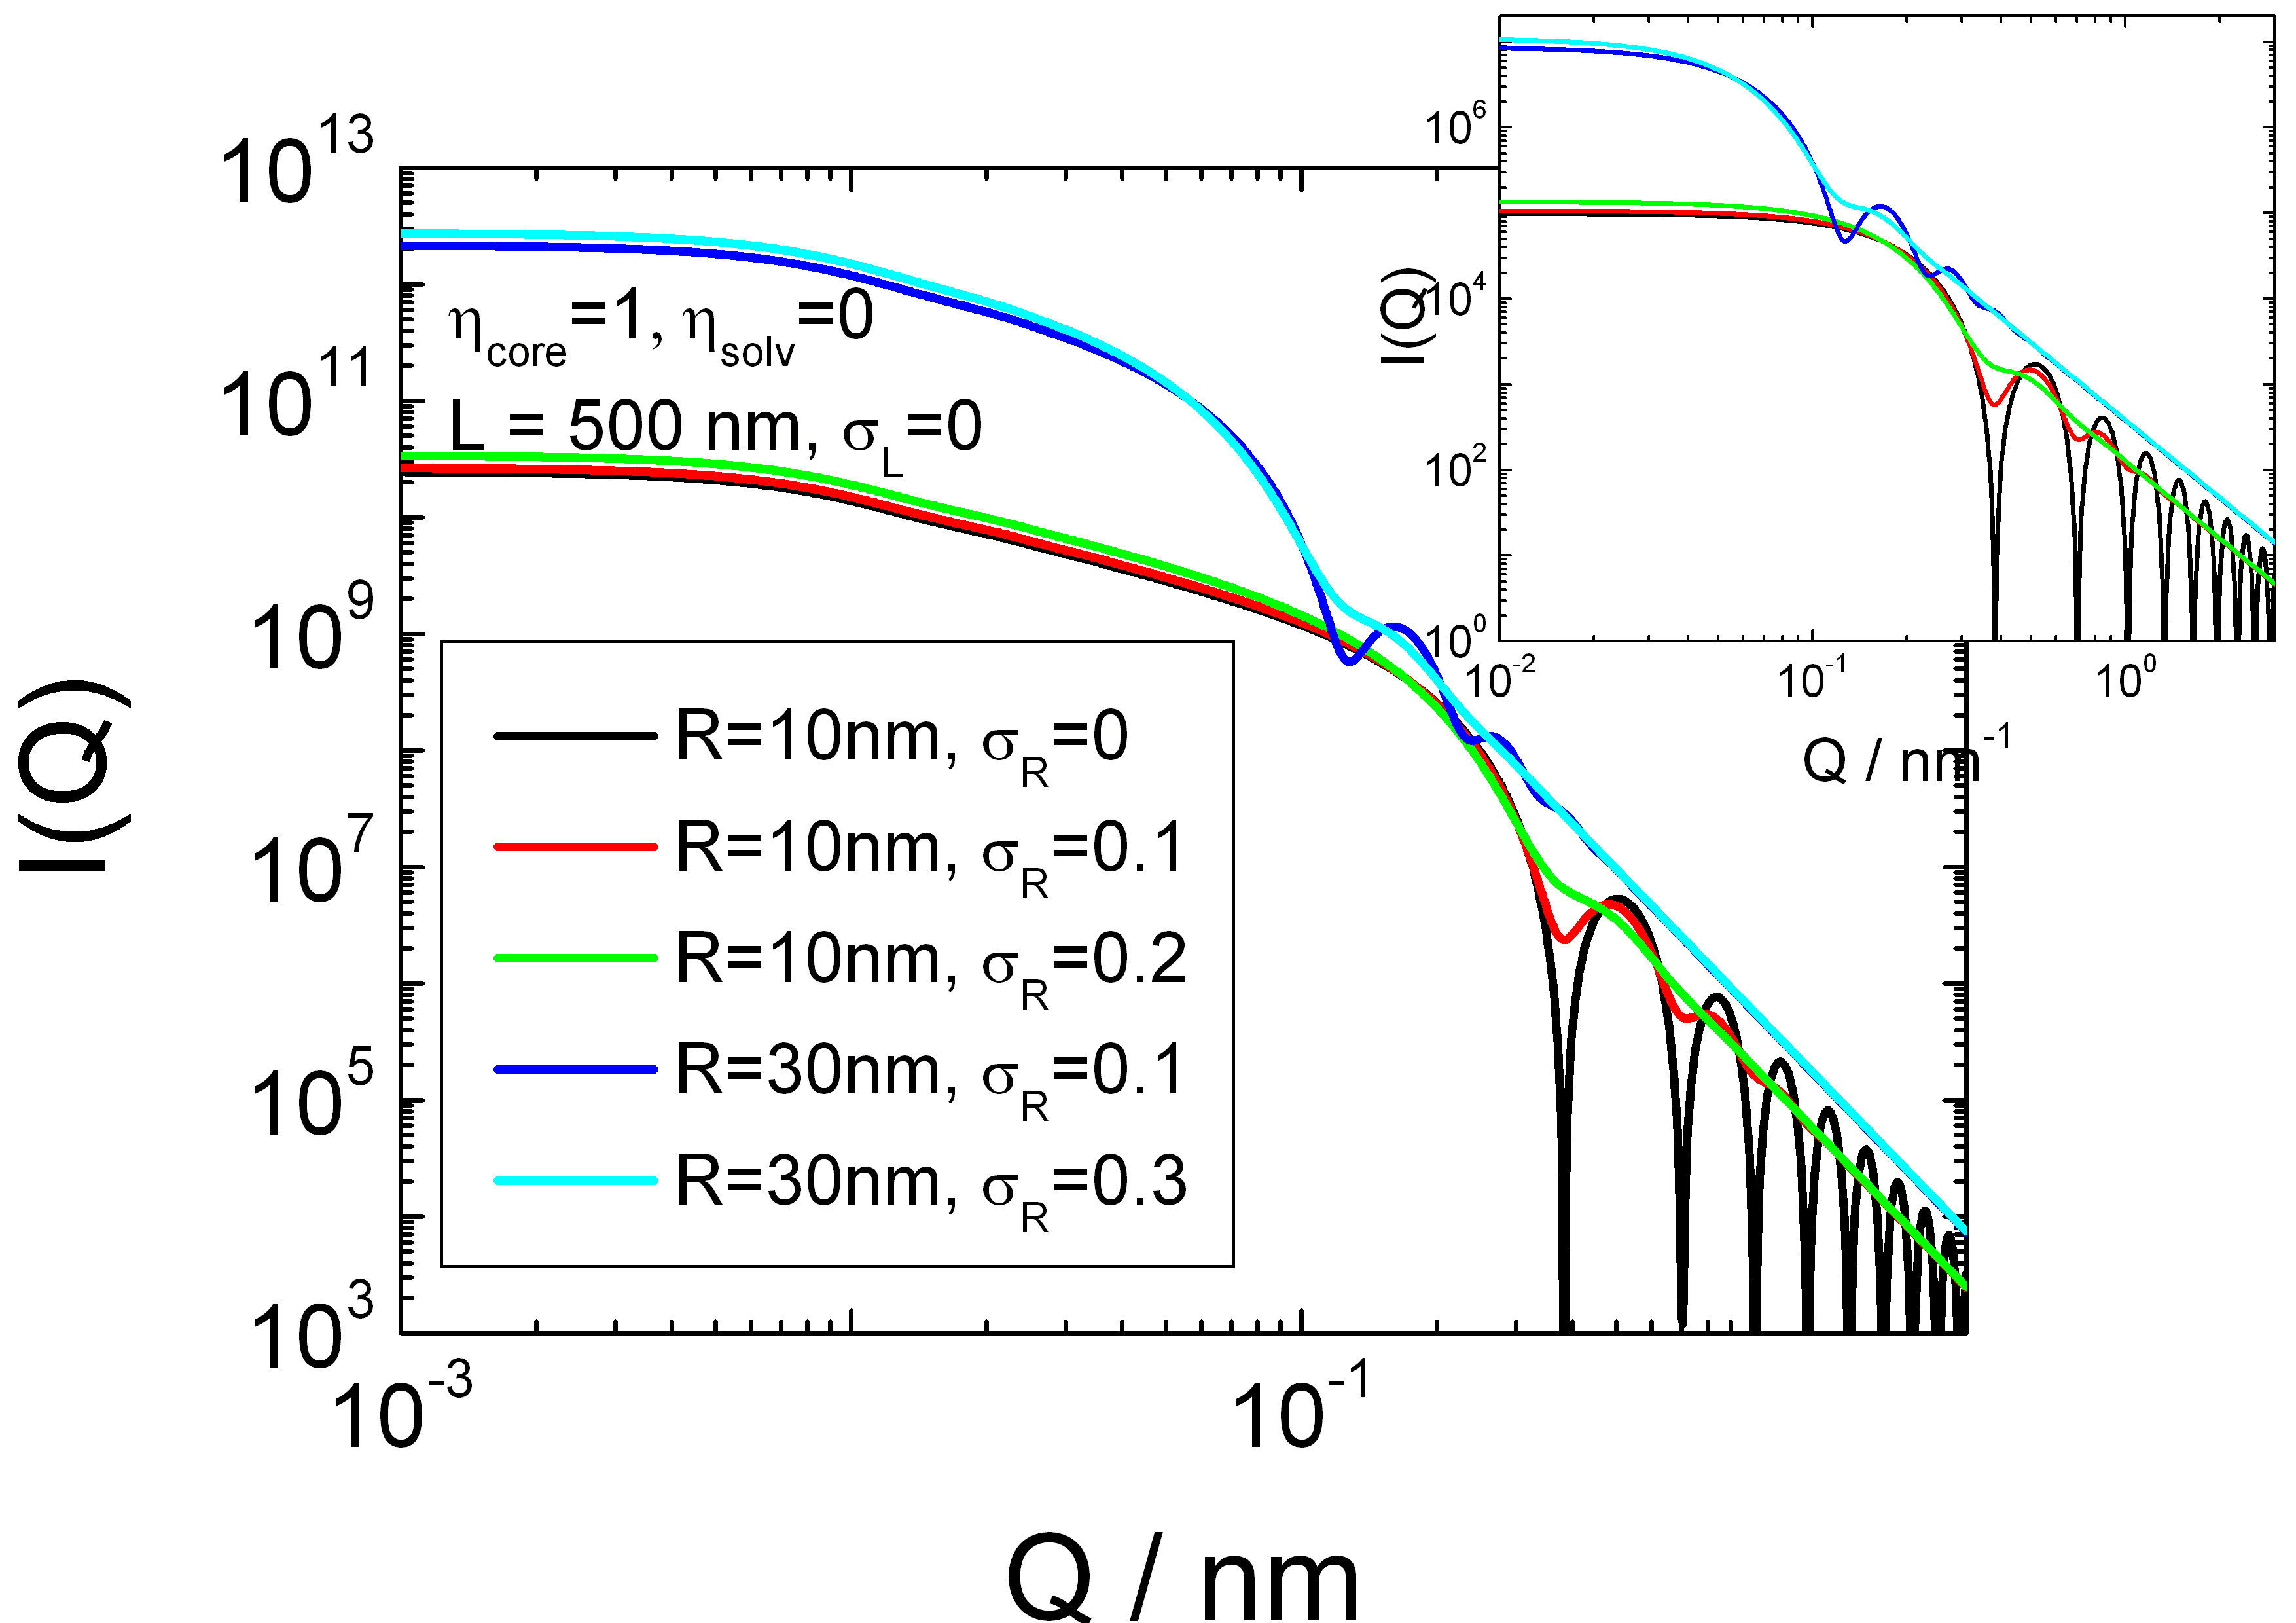
\includegraphics[width=0.8\textwidth,height=0.55\textwidth]{../images/form_factor/anisotropic/CylindricalHomogeneousXSIQ.png}
\end{center}
\caption{Scattering curve for the form factor "\texttt{Pcs:homogeneousCyl}" only (insert) and
in combination with a structure factor "\texttt{P'(Q): Thin Rod}".}
\label{fig_IQ:Pcs:CylindricalHomogeneousXSIQ}
\end{figure}

\clearpage
\subsubsection{Pcs(Q) for cross-section of a cylindrical shell with elliptical cross section} ~\\
\label{plugin:Pcs:CylEllSh}

\noindent
This cross-section form factor describes the scattering of an elliptical core-shell cross-section.
The cross-section radius $R$ can have a distribution with a width of $sigma$ as
described by a log-normal distribution according to eq.\ \ref{eq:LogNormal}.

\begin{equation}
\begin{split}
    P_\textrm{cs}(Q) = & \int_0^\infty \textrm{LogNorm}(t',1,\sigma_{t},1,t)  \quad \int_0^\infty \textrm{LogNorm}(R',1,\sigma_{R_{0}},1,R)  \quad \times\\
        & \int_0^{\pi/2}
\Big[\left( \eta_\textrm{shell}-\eta_\textrm{solv}\right)F_\textrm{cs,ell}(Q,R'+t',\epsilon,\phi) \\
& \quad + \left(\eta_\textrm{core}-\eta_\textrm{shell}\right)F_\textrm{cs,ell}(Q,R',\epsilon,\phi)
\Big]^2 \, \mathrm{d}\phi  \, \mathrm{d}R'  \, \mathrm{d}t'
\end{split} \label{eq:PcsellCylSh}
\end{equation}
with
\begin{subeqnarray}
F_\textrm{cs,ell}\left(Q,R,\epsilon,\Delta\eta\phi\right) &=&  \frac{2 \mathrm{J}_1(Qr(R,\epsilon,\phi))}{Qr(R,\epsilon,\phi)}   \\
r(R,\epsilon,\phi) &=& R\sqrt{\sin^2\phi+\epsilon^2\cos^2\phi}
\end{subeqnarray}



\vspace{5mm}

\hspace{1pt}\\
\underline{Input parameters for \texttt{Pcs:ellCylSh}:}
\begin{description}
    \item[\texttt{R\_0}] most probable radius $R_0$
    \item[\texttt{sigm\_R0}] width $\sigma_{R_0}$ of radius distribution (LogNorm)
    \item[\texttt{epsilon}] eccentricity $\epsilon$ of elliptical cross-section
    \item[\texttt{t}] most probable shell thickness $t$
    \item[\texttt{dummy}] width $\sigma_t$ of shell thickness distribution (LogNorm)
    \item[\texttt{dummy}] not used
    \item[\texttt{dummy}] not used
    \item[\texttt{eta\_core}] scattering length density of the core $\eta_\textrm{core}$
    \item[\texttt{eta\_shell}] scattering length density of the shell $\eta_\textrm{shell}$
    \item[\texttt{eta\_solv}] scattering length density of the solvent $\eta_\textrm{solv}$
\end{description}

\noindent
\underline{Note}
\begin{itemize}
  \item This form factor is supposed to be combined with a shape factor for
local cylindrical objects which are implemented as structure  plugins
under "\texttt{[by plugin|thin obj.|P'(Q): local cylindrical obj.]}".
\item As the form factor already has the width distribution included one normally uses in \SASfit as a size distribution
the \texttt{Delta}-distribution.
\end{itemize}

\begin{figure}[htb]
\begin{center}
\subfigure[Plot of the cross section form factor $P_\text{cs}$ in combination with a structure factor "\texttt{P'(Q): Rod}" as the shape factor $P'(Q)$.]{
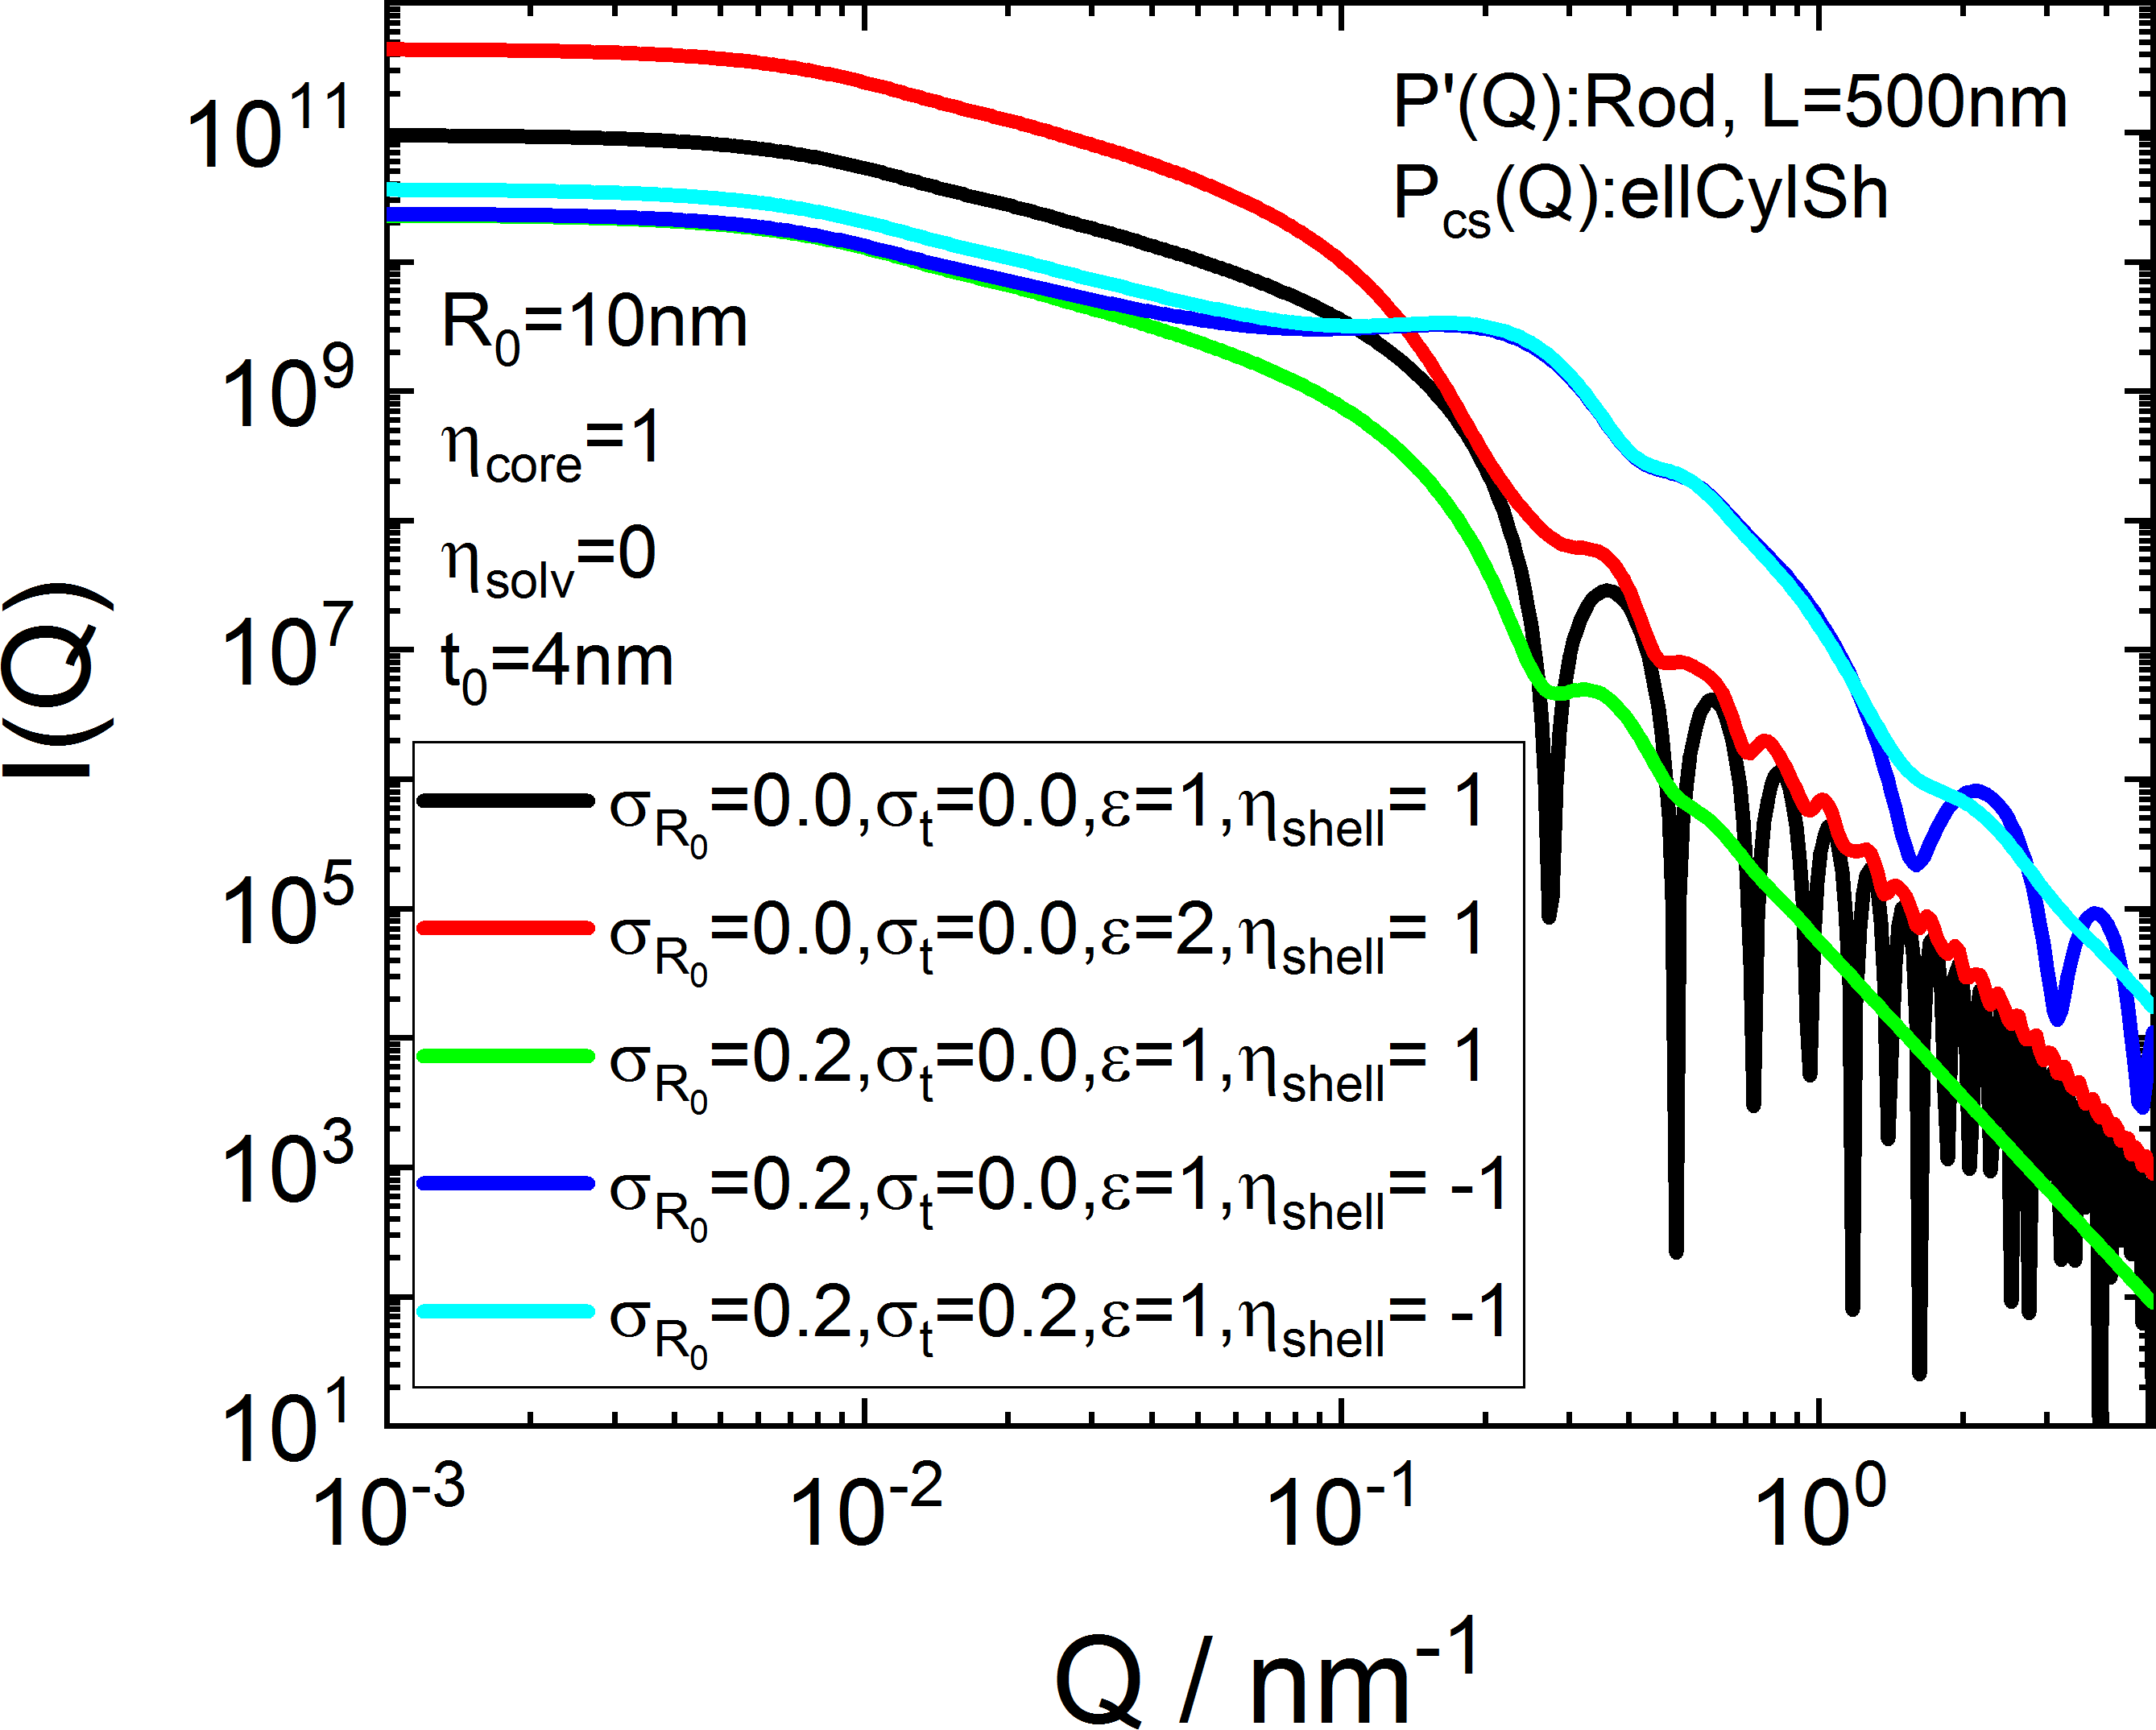
\includegraphics[width=0.48\textwidth,height=0.35\textwidth]{../images/form_factor/anisotropic/ellCylShIQa.png}}
\hfill
\subfigure[Plot of the cross section form factor $P_\text{cs}$ only according to eq.\ \ref{eq:PcsellCylSh}.
The parameters for the profile are the same than in Fig.\ \ref{fig:ellCylShIQ}a]{
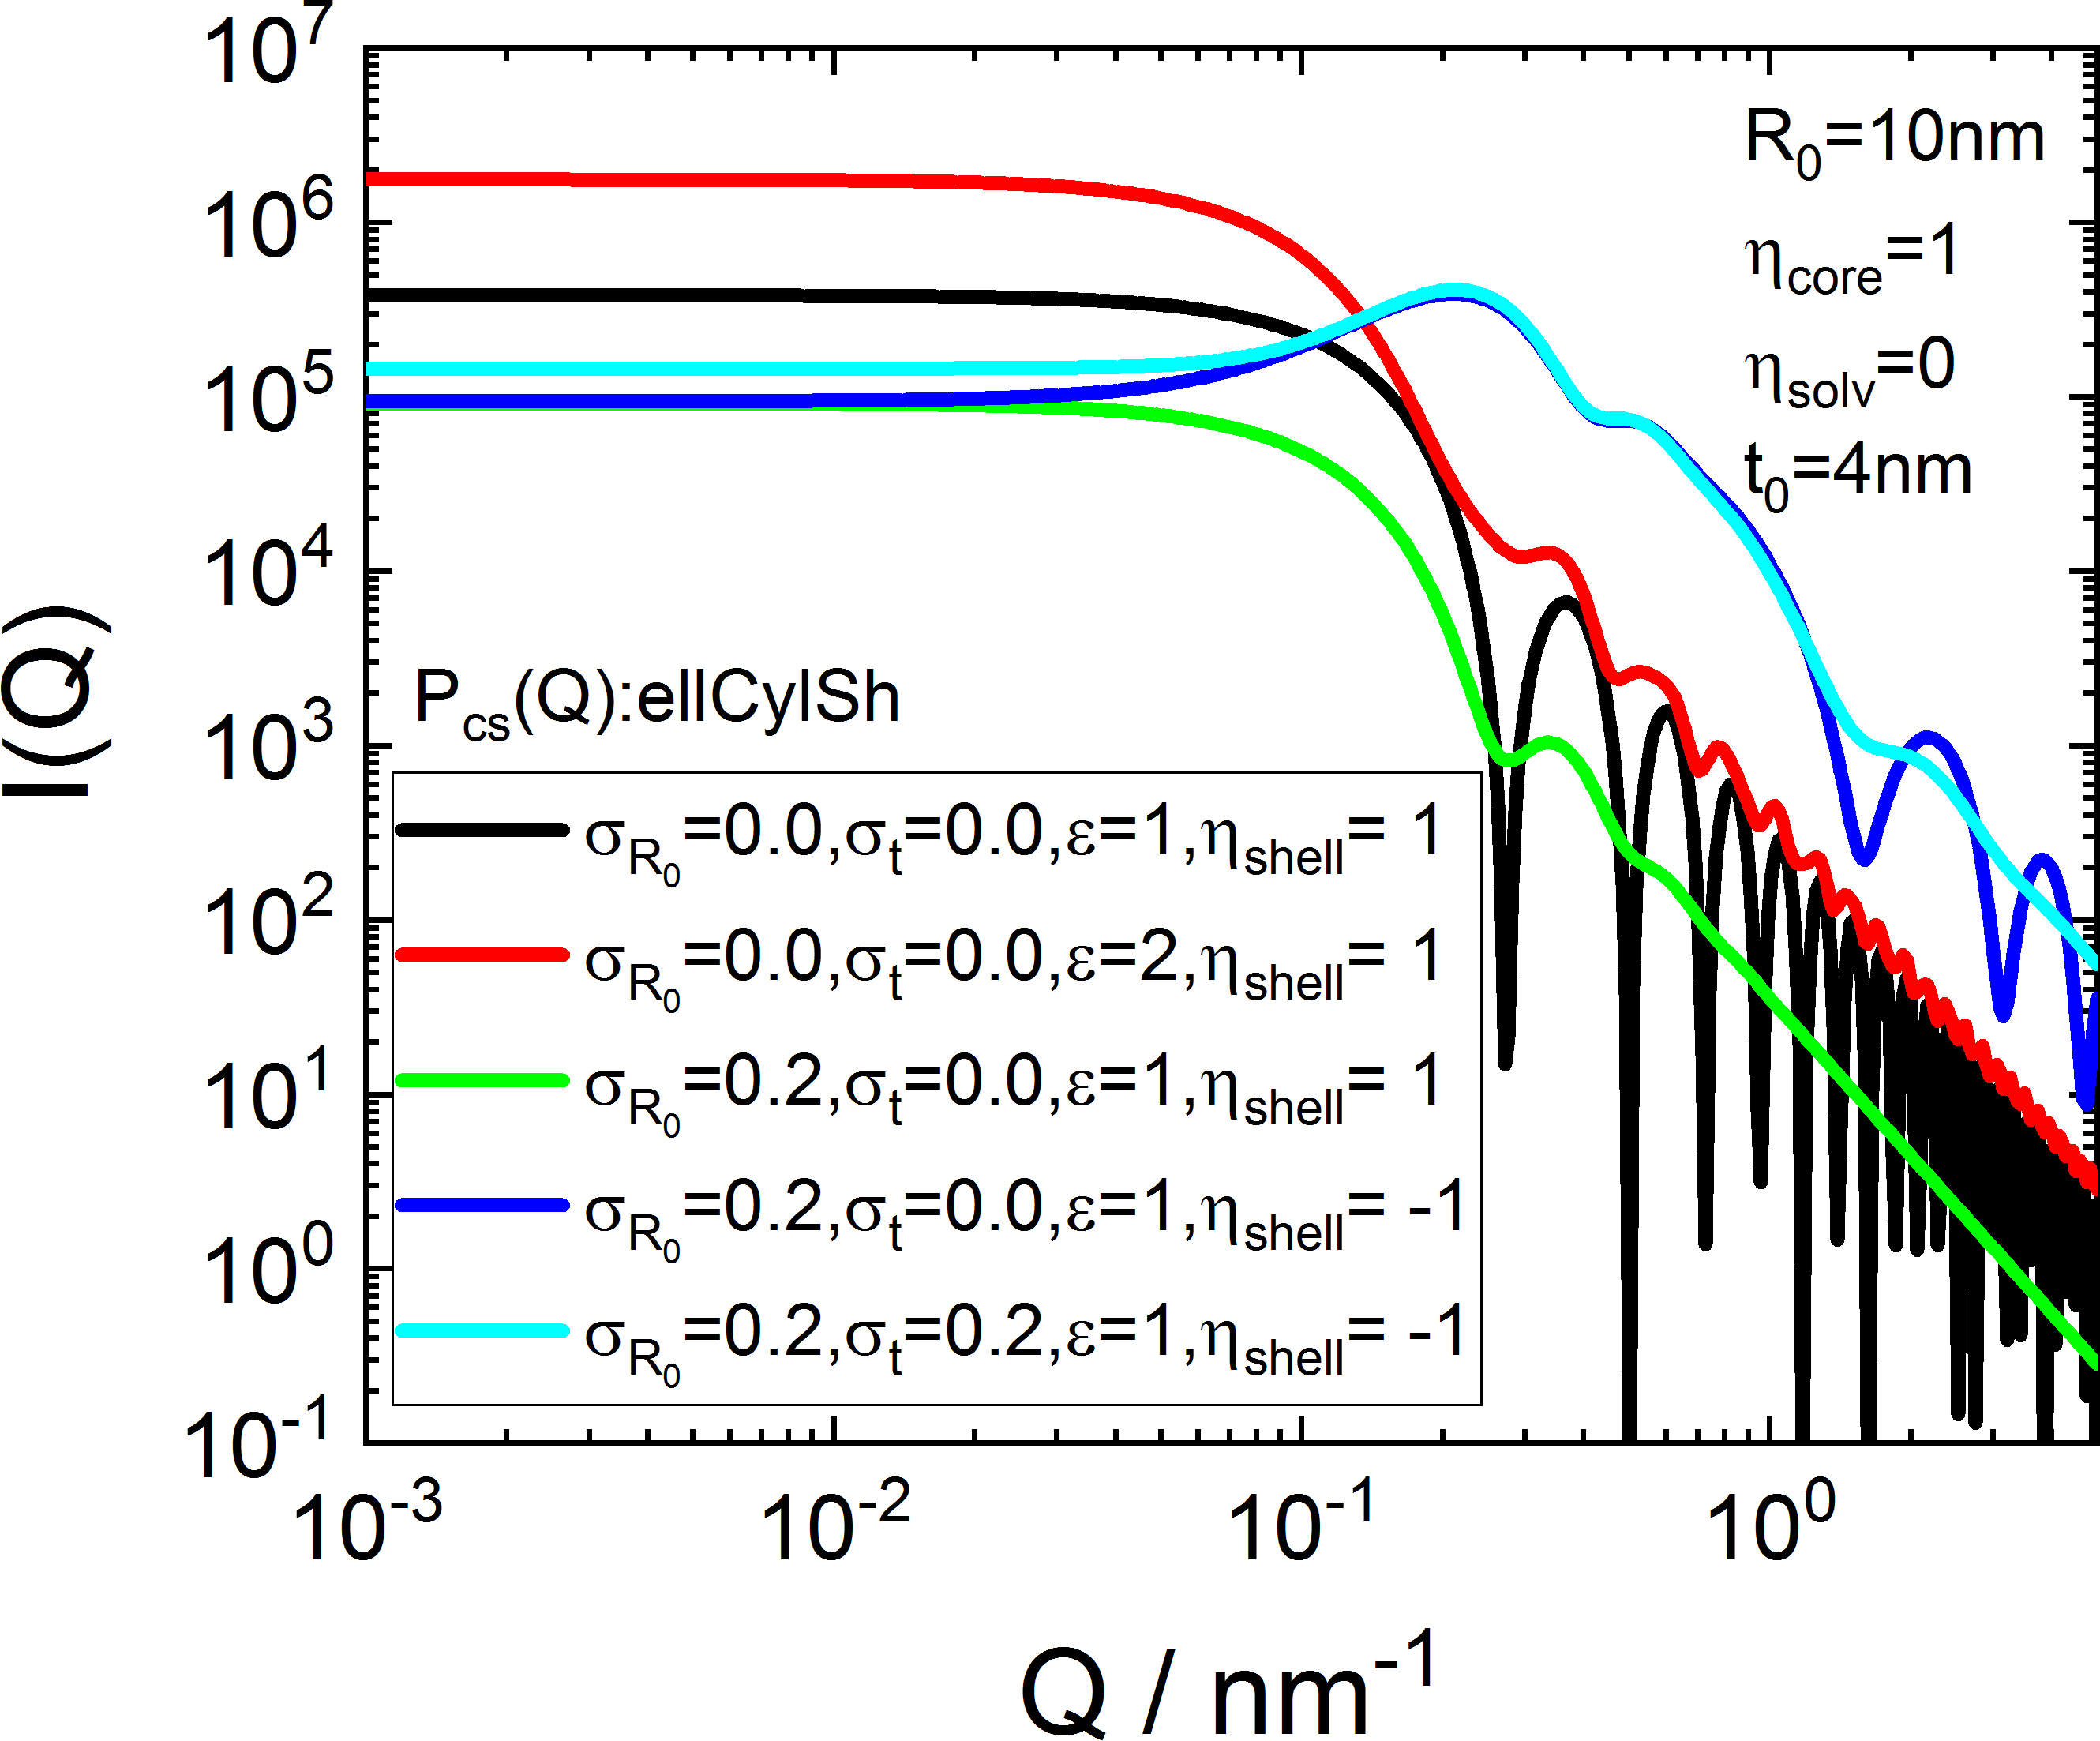
\includegraphics[width=0.48\textwidth,height=0.35\textwidth]{../images/form_factor/anisotropic/ellCylShIQb.png}}
\end{center}
\caption{Scattering curve for the cross-section form factor "\texttt{Pcs:ellCylSh}".}
\label{fig:ellCylShIQ}
\end{figure}


\clearpage
\subsection{P'(Q) for local planar obj.} ~\\
\label{plugin:Pprime4planar}

As local planar objects the following shapes have been implemented:
\begin{enumerate}
\item thin disc
\item thin spherical shell
\item thin ellipsoidal shell
\item thin hollow cylinder with closed ends
\end{enumerate}

\clearpage
\subsubsection{P'(Q): thin discs} ~\\
\label{plugin:Pprime4Discs}

\begin{figure}[htb]
\begin{center}
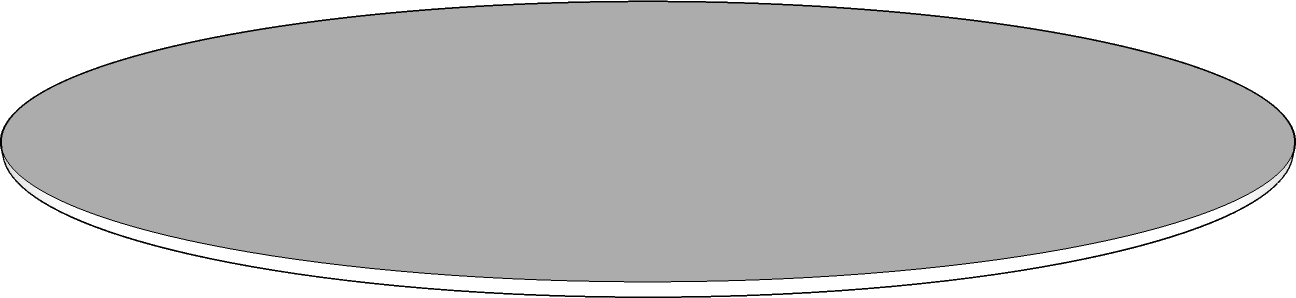
\includegraphics[width=0.686\textwidth,height=0.27\textwidth]{../images/form_factor/anisotropic/ThinDisc.png}
\end{center}
\caption{Sketch of a thin disc with a radius $R$. The thickness of the disc is assumed to be much smaller than its radius.}
\label{fig:ThinDisc}
\end{figure}
\begin{align}
P'(Q) &= \int_0^\infty \mathrm{LogNorm}(R',\sigma,1,R) \,\pi^2R'^4\frac{2}{\left(R'Q\right)^2}\left(1-\frac{2\mathrm{J}_1(2QR')}{2QR'}\right) \, \mathrm{d} R'
\label{eq:PprimeThinDisc}
\end{align}

\vspace{5mm}

\hspace{1pt}\\
\underline{Input parameters for \texttt{P'(Q): Thin Disc}:}
\begin{description}
    \item[\texttt{R}] most probable radius $R$
    \item[\texttt{dummy}] not used
    \item[\texttt{sigma}] width $\sigma$ of radius distribution (LogNorm)
\end{description}

\noindent
\underline{Note}
\begin{itemize}
  \item This structure factor is supposed to be combined with a form factor of local planar objects which are implemented as form factor plugins
under "\texttt{[by plugin|thin obj.|Pcs(Q): local planar obj.]}".
\item The structure factor already has a log-normal width distribution for one parameter included.
\end{itemize}

\begin{figure}[htb]
\begin{center}
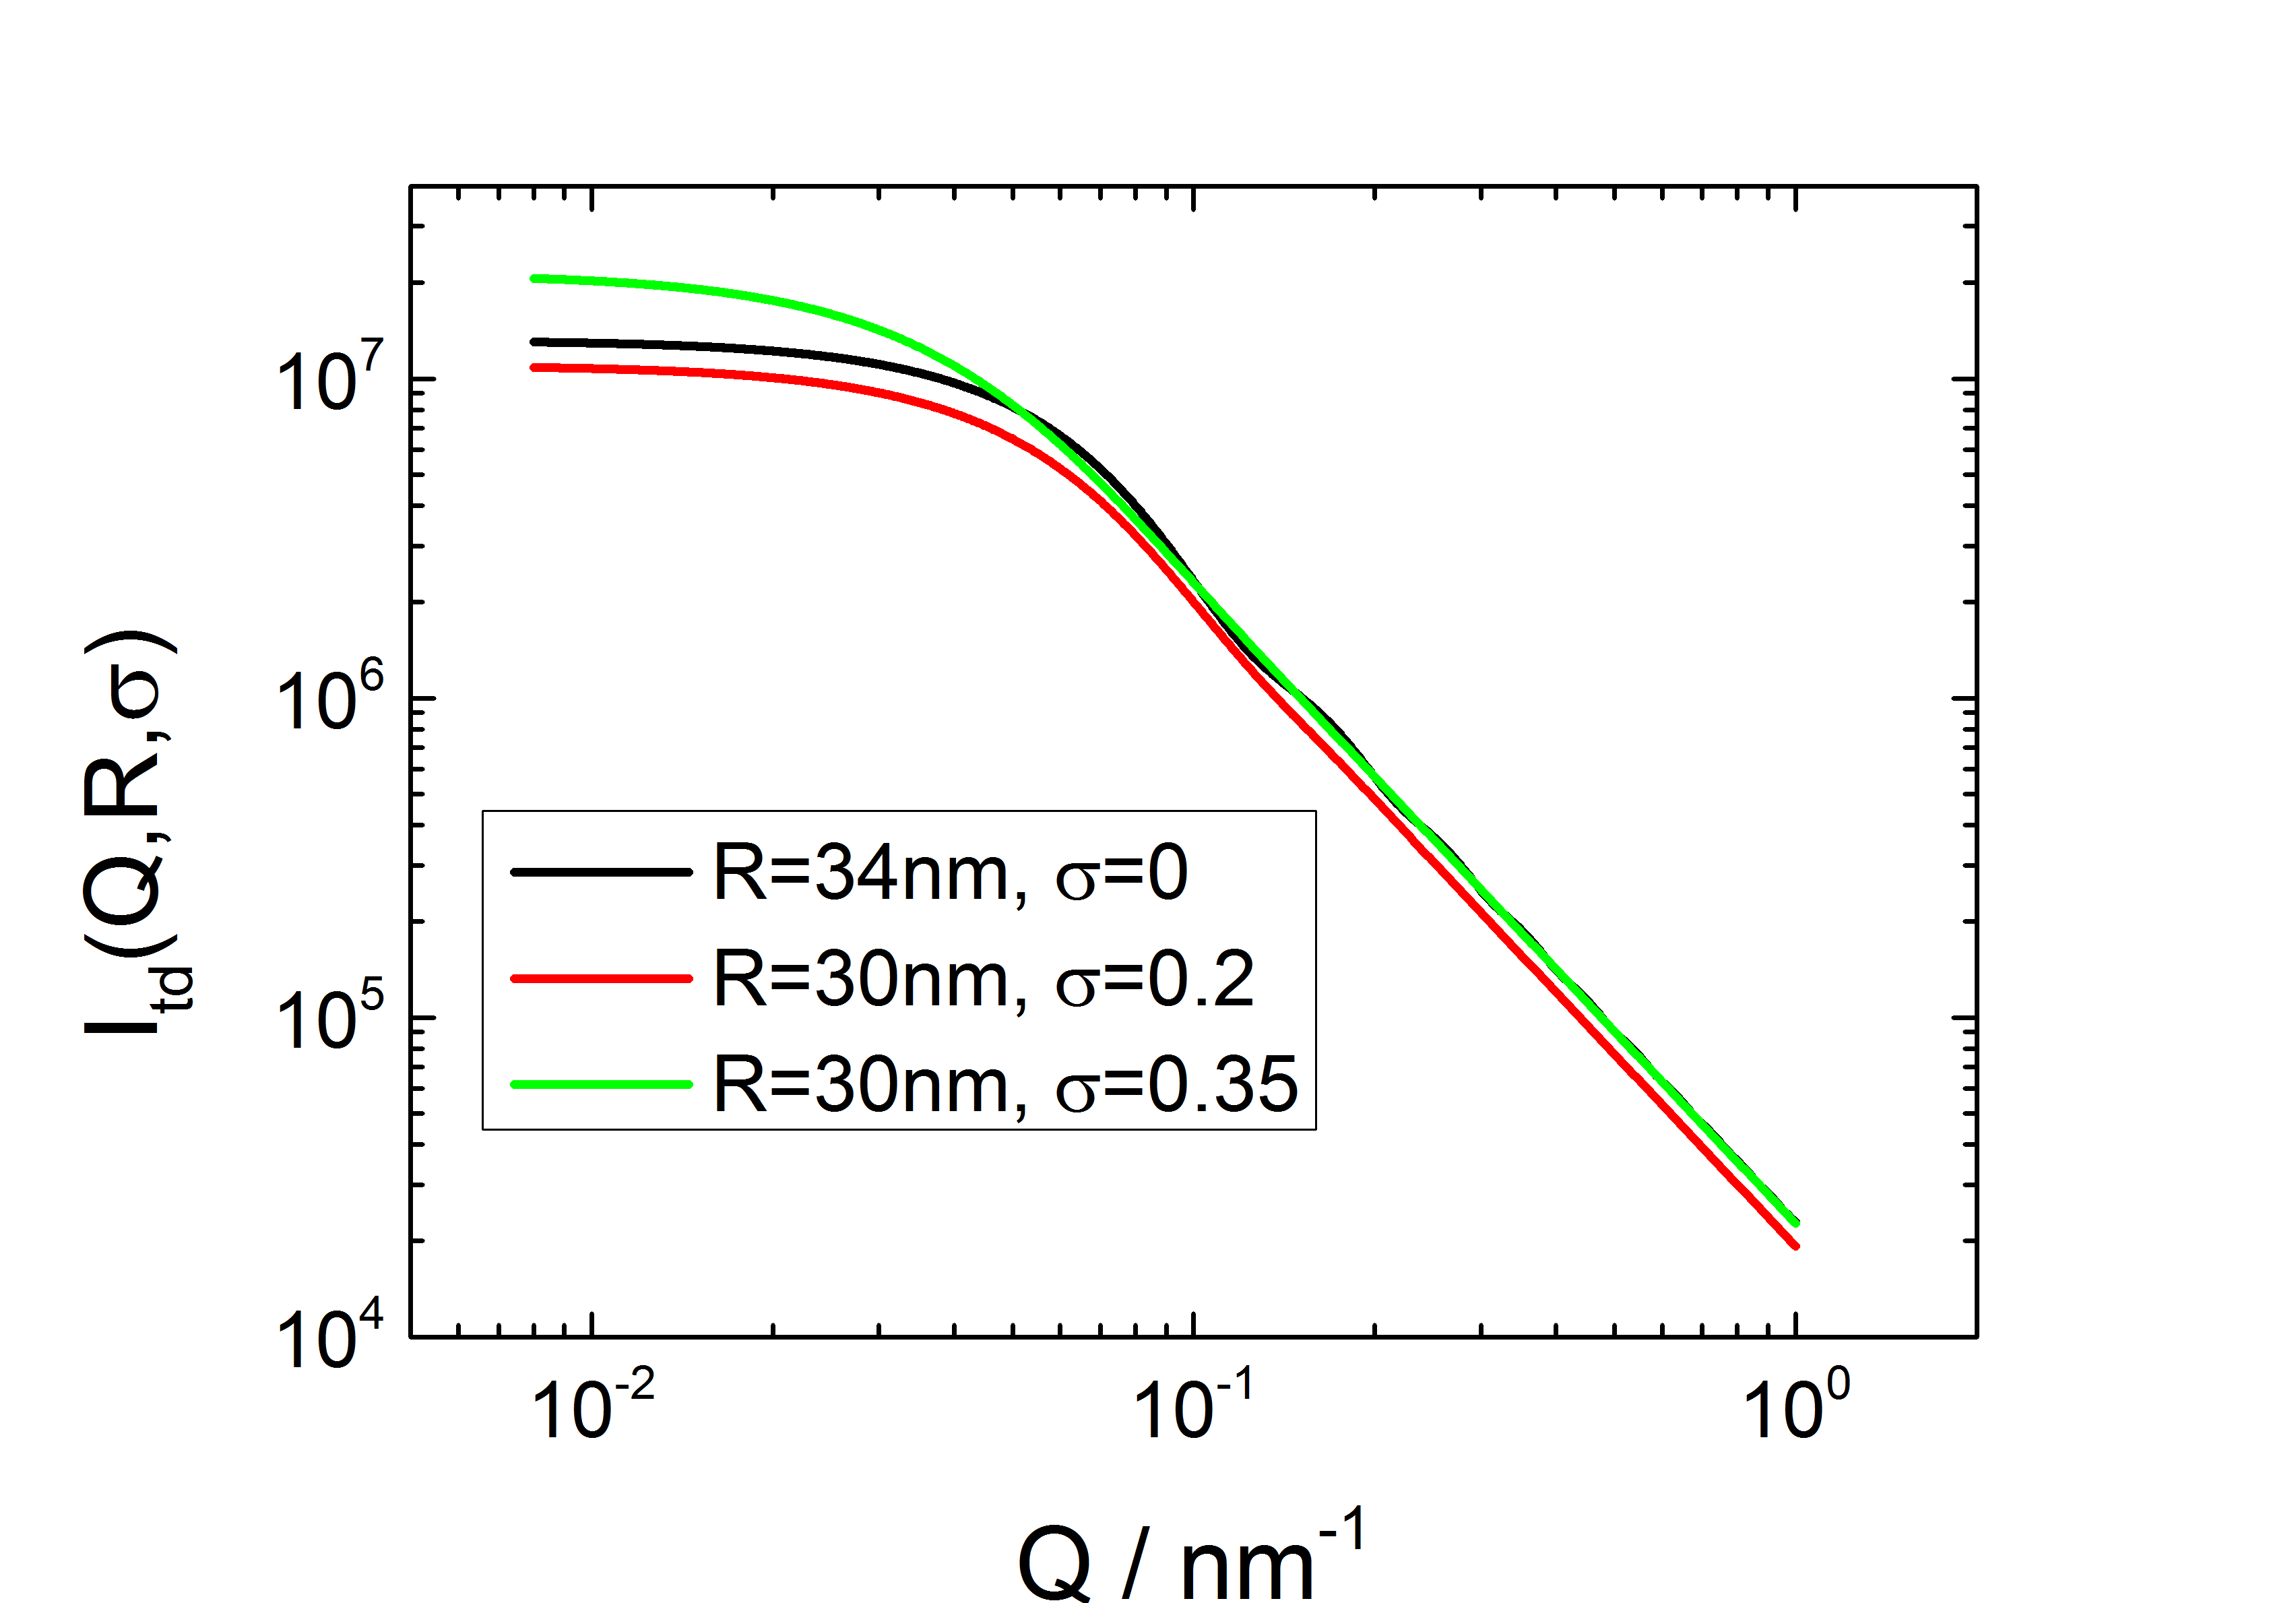
\includegraphics[width=0.8\textwidth,height=0.55\textwidth]{../images/form_factor/anisotropic/PprimeThinDisc.png}
\end{center}
\caption{Scattering curve for the structure factor "\texttt{P'(Q): Thin Disc}" in combination with a constant background of 1".}
\label{fig_IQ:PprimeThinDisc}
\end{figure}

\clearpage
\subsubsection{P'(Q): thin spherical shell} ~\\
\label{plugin:Pprime4spShell}

\begin{figure}[htb]
\begin{center}
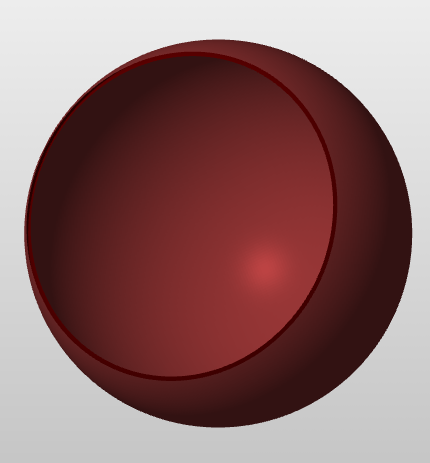
\includegraphics[width=0.43\textwidth,height=0.463\textwidth]{../images/form_factor/anisotropic/Sphere_thin.png}
\end{center}
\caption{Sketch of a thin spherical shell with a radius $R$. The thickness of the shell is assumed to be much smaller than the radius of the sphere.}
\label{fig:ThinSphericalShell}
\end{figure}
\begin{align}
P'(Q) &= \int_0^\infty \, \mathrm{LogNorm}(R',\sigma,1,R)\, \left(4\pi R'^2\frac{\sin(QR')}{QR'}\right)^2 \mathrm{d}R'
\label{eq:PprimeSphSh}
\end{align}

\vspace{5mm}

\hspace{1pt}\\
\underline{Input parameters for \texttt{P'(Q): Thin Spherical Shell}:}
\begin{description}
    \item[\texttt{R}] most probable radius $R$
    \item[\texttt{dummy}] not used
    \item[\texttt{sima}] width $\sigma$ of radius distribution (LogNorm)
\end{description}

\noindent
\underline{Note}
\begin{itemize}
  \item This structure factor is supposed to be combined with a form factor of local planar objects which are implemented as form factor plugins
under "\texttt{[by plugin|thin obj.|Pcs(Q): local planar obj.]}".
\item The structure factor already has a log-normal width distribution for one parameter included.
\end{itemize}

\begin{figure}[htb]
\begin{center}
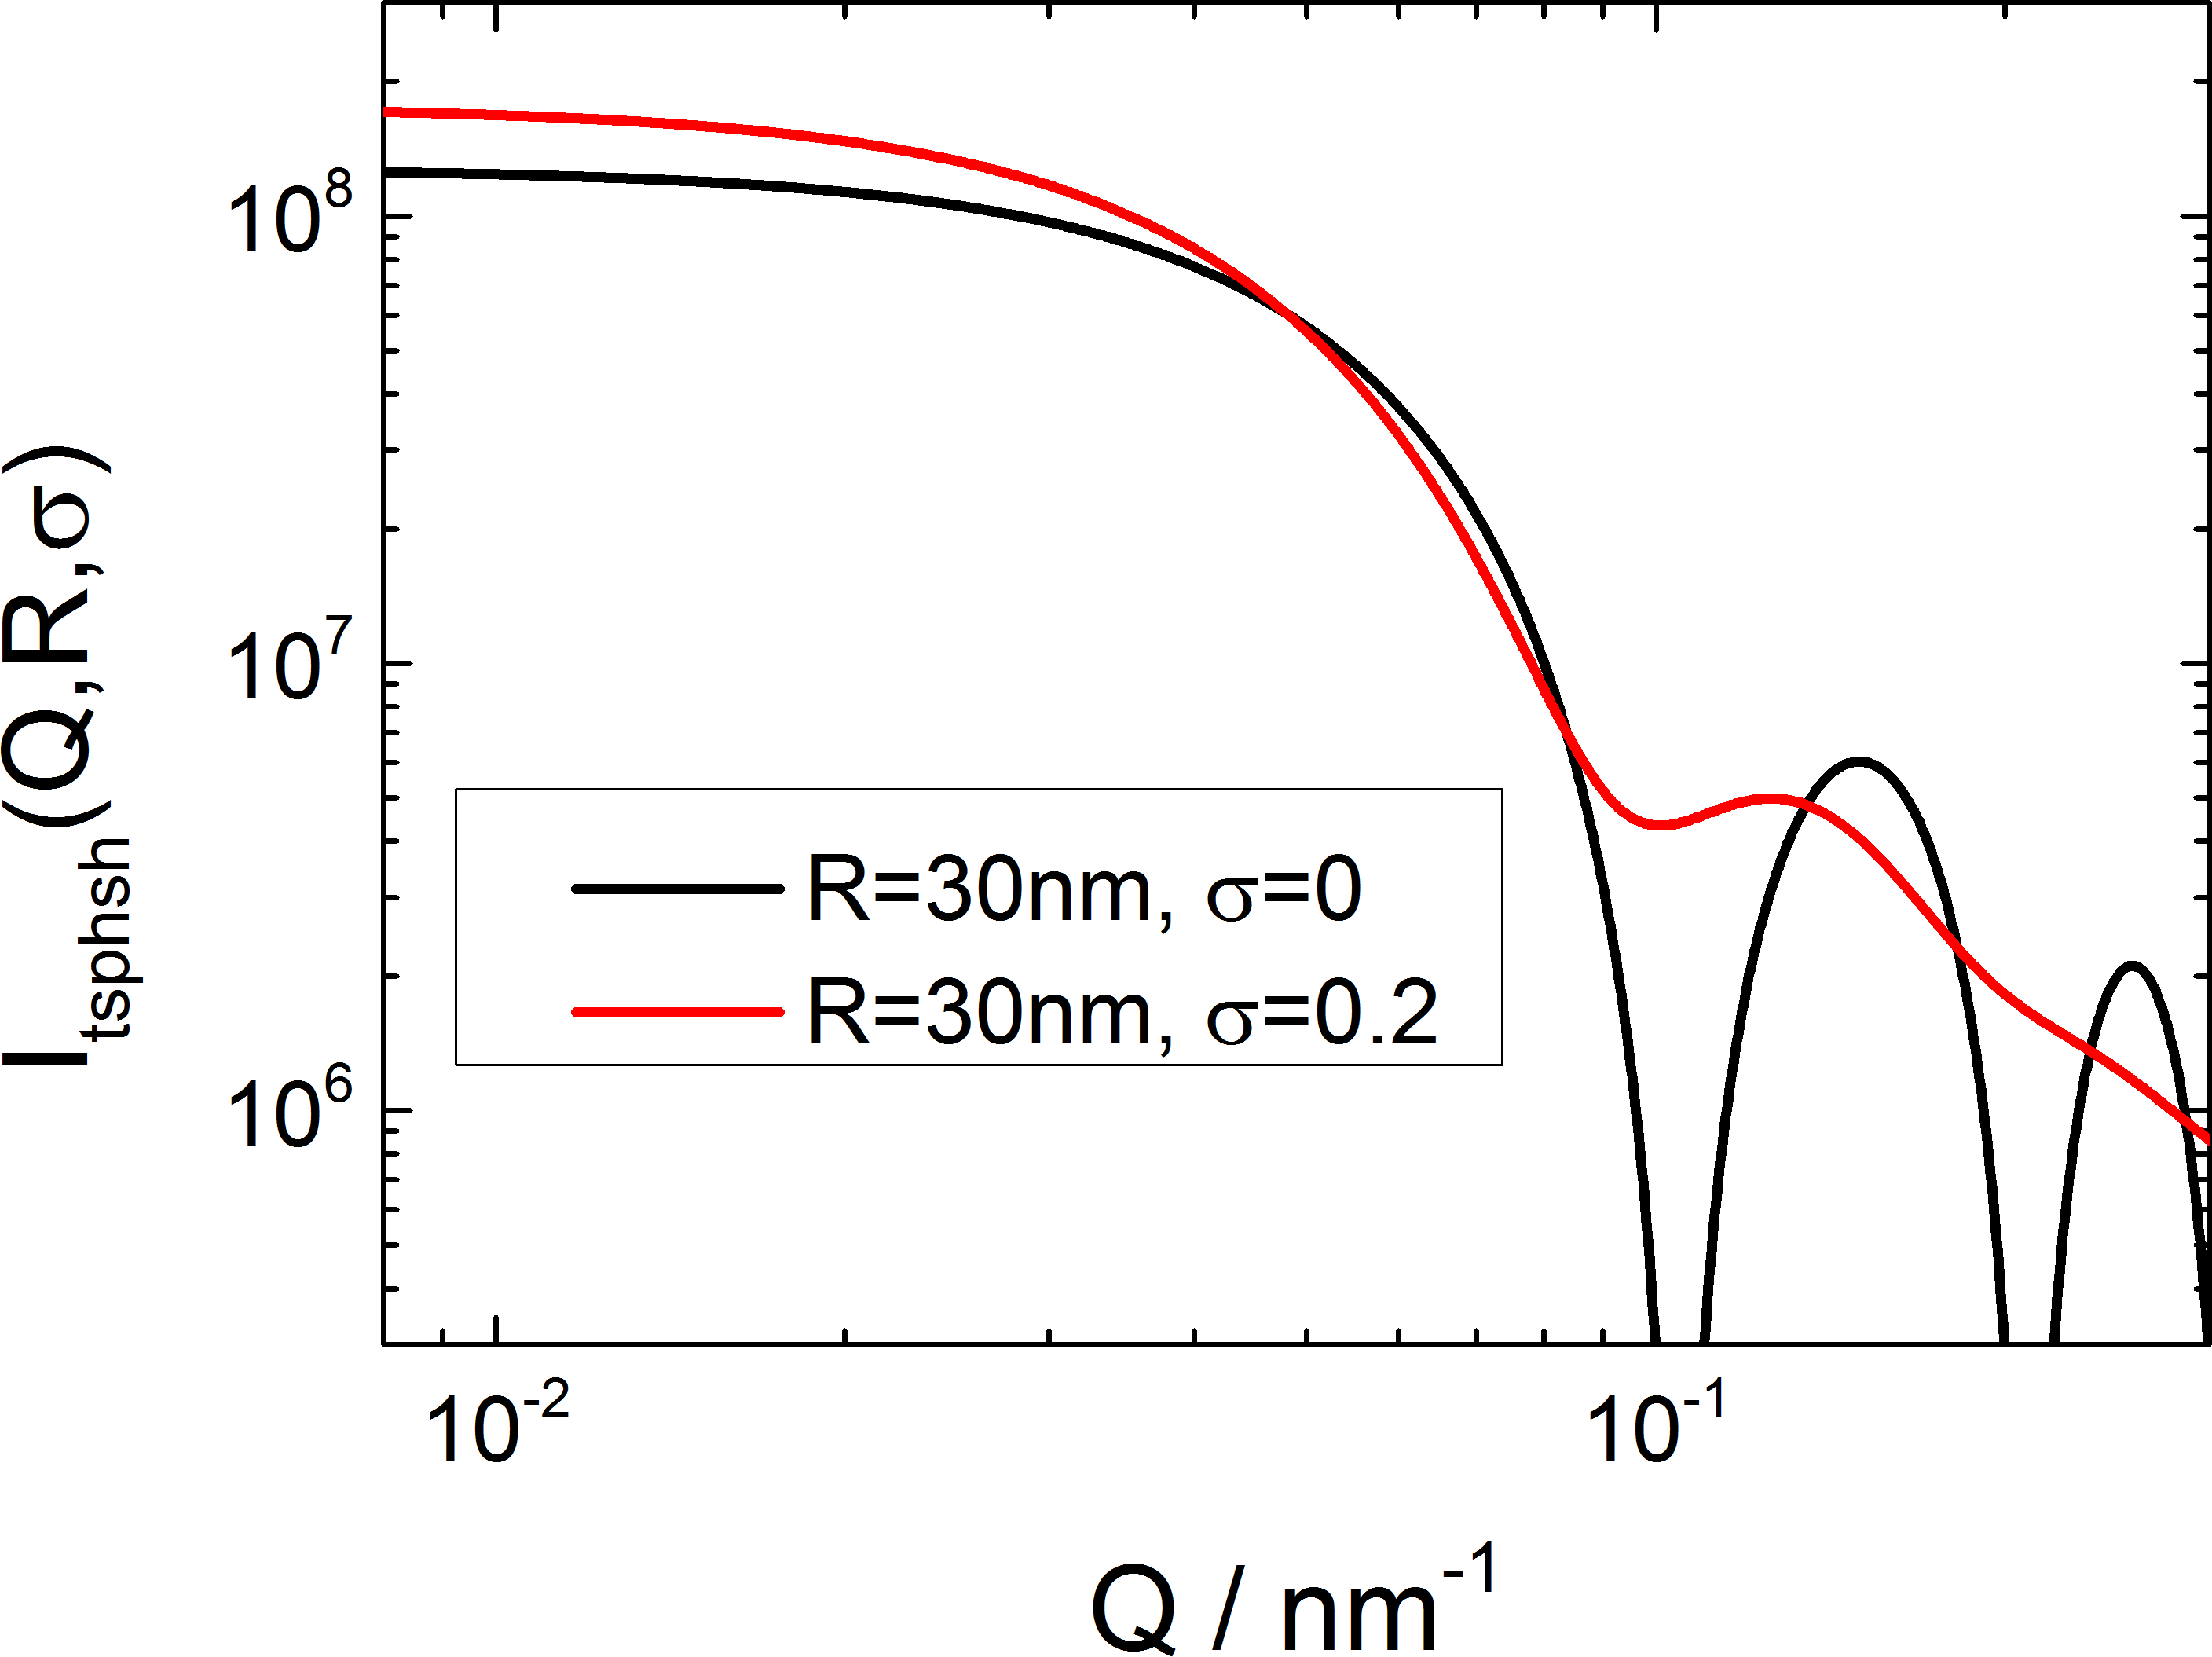
\includegraphics[width=0.8\textwidth,height=0.55\textwidth]{../images/form_factor/anisotropic/PprimeThinSphShell.png}
\end{center}
\caption{Scattering curve for the structure factor "\texttt{P'(Q): Thin Spherical Shell}" in combination with a constant background of 1".}
\label{fig_IQ:PprimeThinSphShell}
\end{figure}


\clearpage
\subsubsection{P'(Q): thin ellipsoidal shell} ~\\
\label{plugin:Pprime4ellShell}

\begin{figure}[htb]
\begin{center}
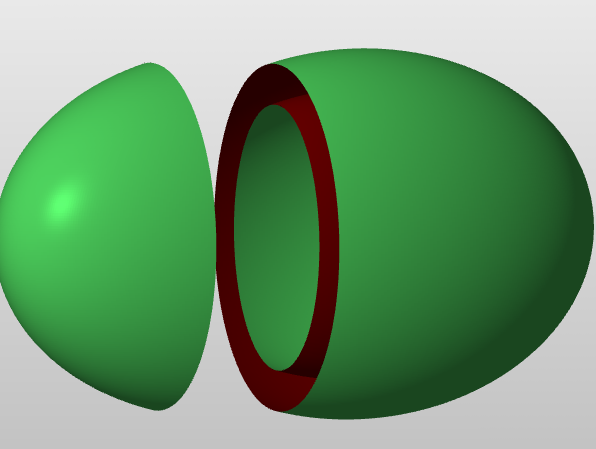
\includegraphics[width=0.596\textwidth,height=0.449\textwidth]{../images/form_factor/anisotropic/Ellipsoid_hollow.png}
\end{center}
\caption{Sketch of a thin ellipsoidal shell with a radius $R$ and eccentricity $\epsilon$. The thickness of the shell is assumed to be much smaller than the two radii of the elliptical shell.}
\label{fig:ThinEllipsoidalShell}
\end{figure}

\begin{align}
\mathrm{S}(R,\epsilon) &= 2\pi R^2\left(1+\epsilon^2 {}_2F_1\left(\frac12,1;\frac32;1-\epsilon^2\right)\right) \\
u &= QR'\sqrt{\sin^2\alpha+\epsilon^2\cos^2\alpha} \\
P'(Q,R,\epsilon) &=  \int_0^\infty \mathrm{LogNorm}(R',\sigma,1,R)\, \mathrm{S}^2(R',\epsilon) \mathrm{j}_0^2(Qu)\sin\alpha \, \mathrm{d}\alpha\,\mathrm{d}R'
\label{eq:PprimeEllSh}
\end{align}
with $\mathrm{j}_0$ being the regular spherical Bessel function of zeroth order.

\vspace{5mm}

\hspace{1pt}\\
\underline{Input parameters for \texttt{P'(Q): Thin Ellipsoidal Shell}:}
\begin{description}
    \item[\texttt{R}] most probable radius $R$
    \item[\texttt{epsilon}] eccentricity $\epsilon$
    \item[\texttt{sima\_R}] width $\sigma_R$ of radius distribution (LogNorm)
\end{description}

\noindent
\underline{Note}
\begin{itemize}
  \item This structure factor is supposed to be combined with a form factor of local planar objects which are implemented as form factor plugins
under "\texttt{[by plugin|thin obj.|Pcs(Q): local planar obj.]}".
\item The structure factor already has a log-normal width distribution for one parameter included.
\end{itemize}

\begin{figure}[htb]
\begin{center}
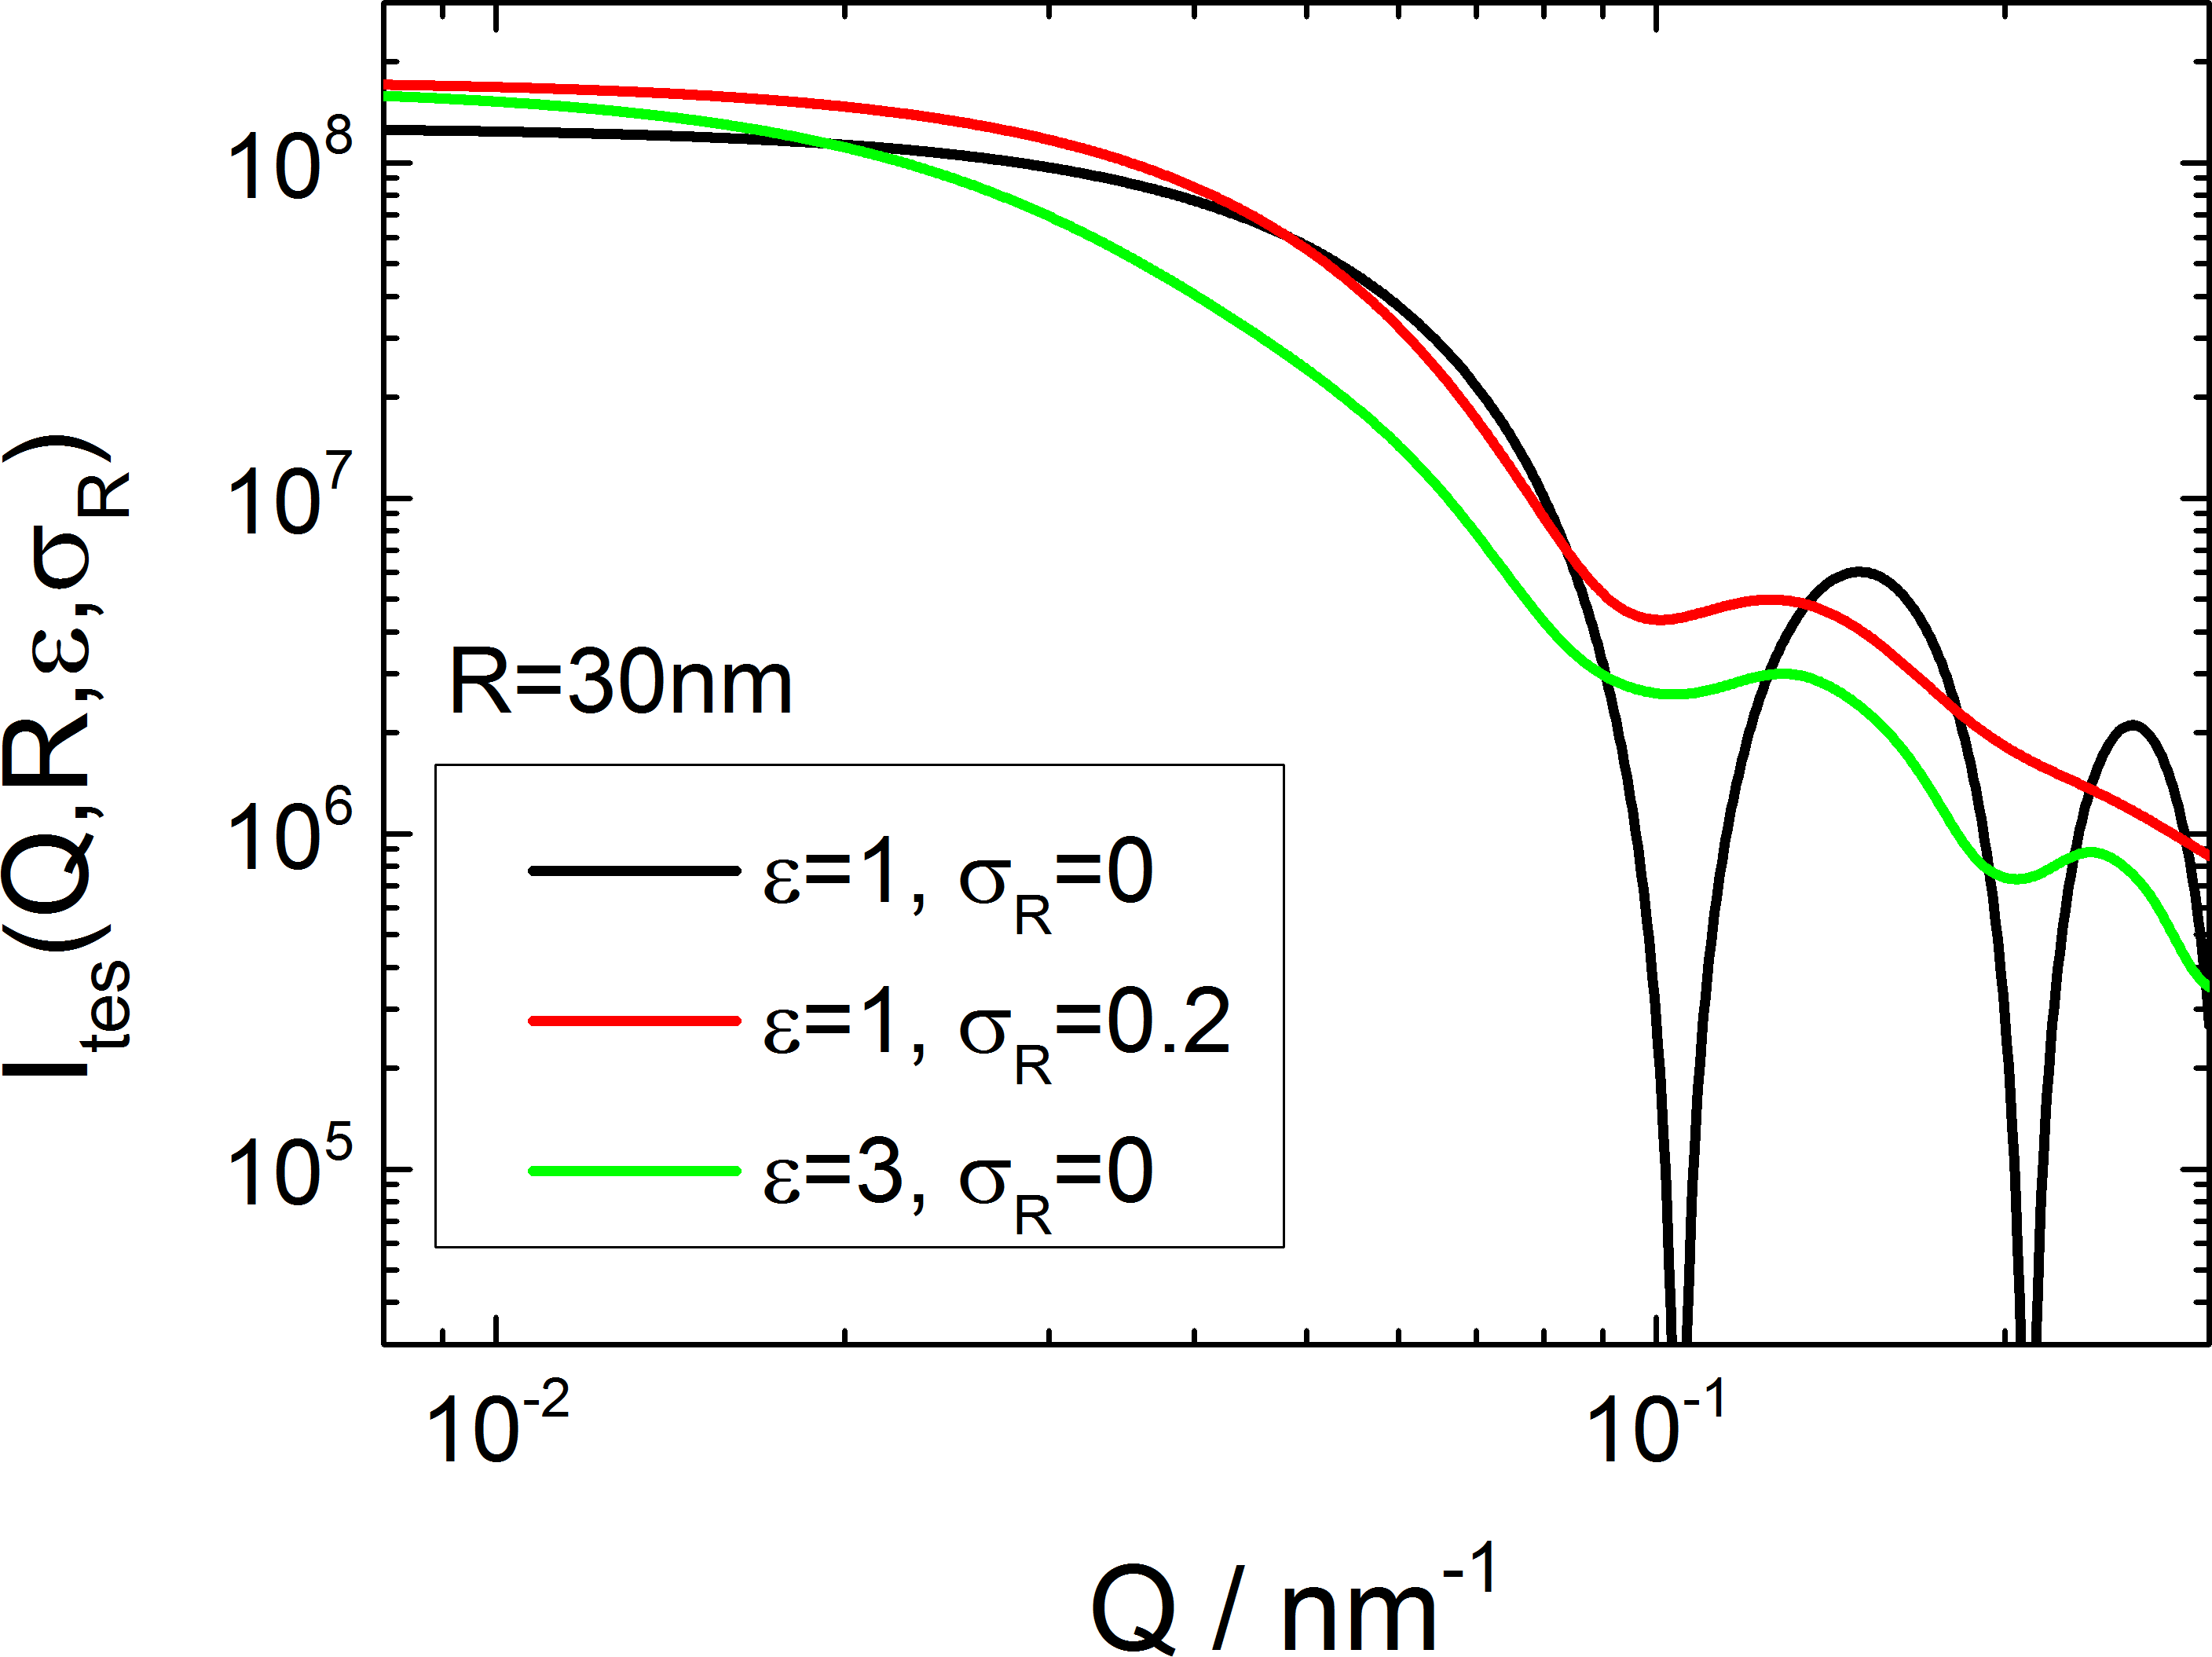
\includegraphics[width=0.8\textwidth,height=0.55\textwidth]{../images/form_factor/anisotropic/PprimeThinEllShell.png}
\end{center}
\caption{Scattering curve for the structure factor "\texttt{P'(Q): Thin Ellipsoidal Shell}" in combination with a constant background of 1".}
\label{fig_IQ:PprimeThinEllShell}
\end{figure}

\clearpage
\subsubsection{P'(Q): thin-walled hollow cylinder} ~\\
\label{plugin:Pprime4hollowcylinder}

\begin{figure}[htb]
\begin{center}
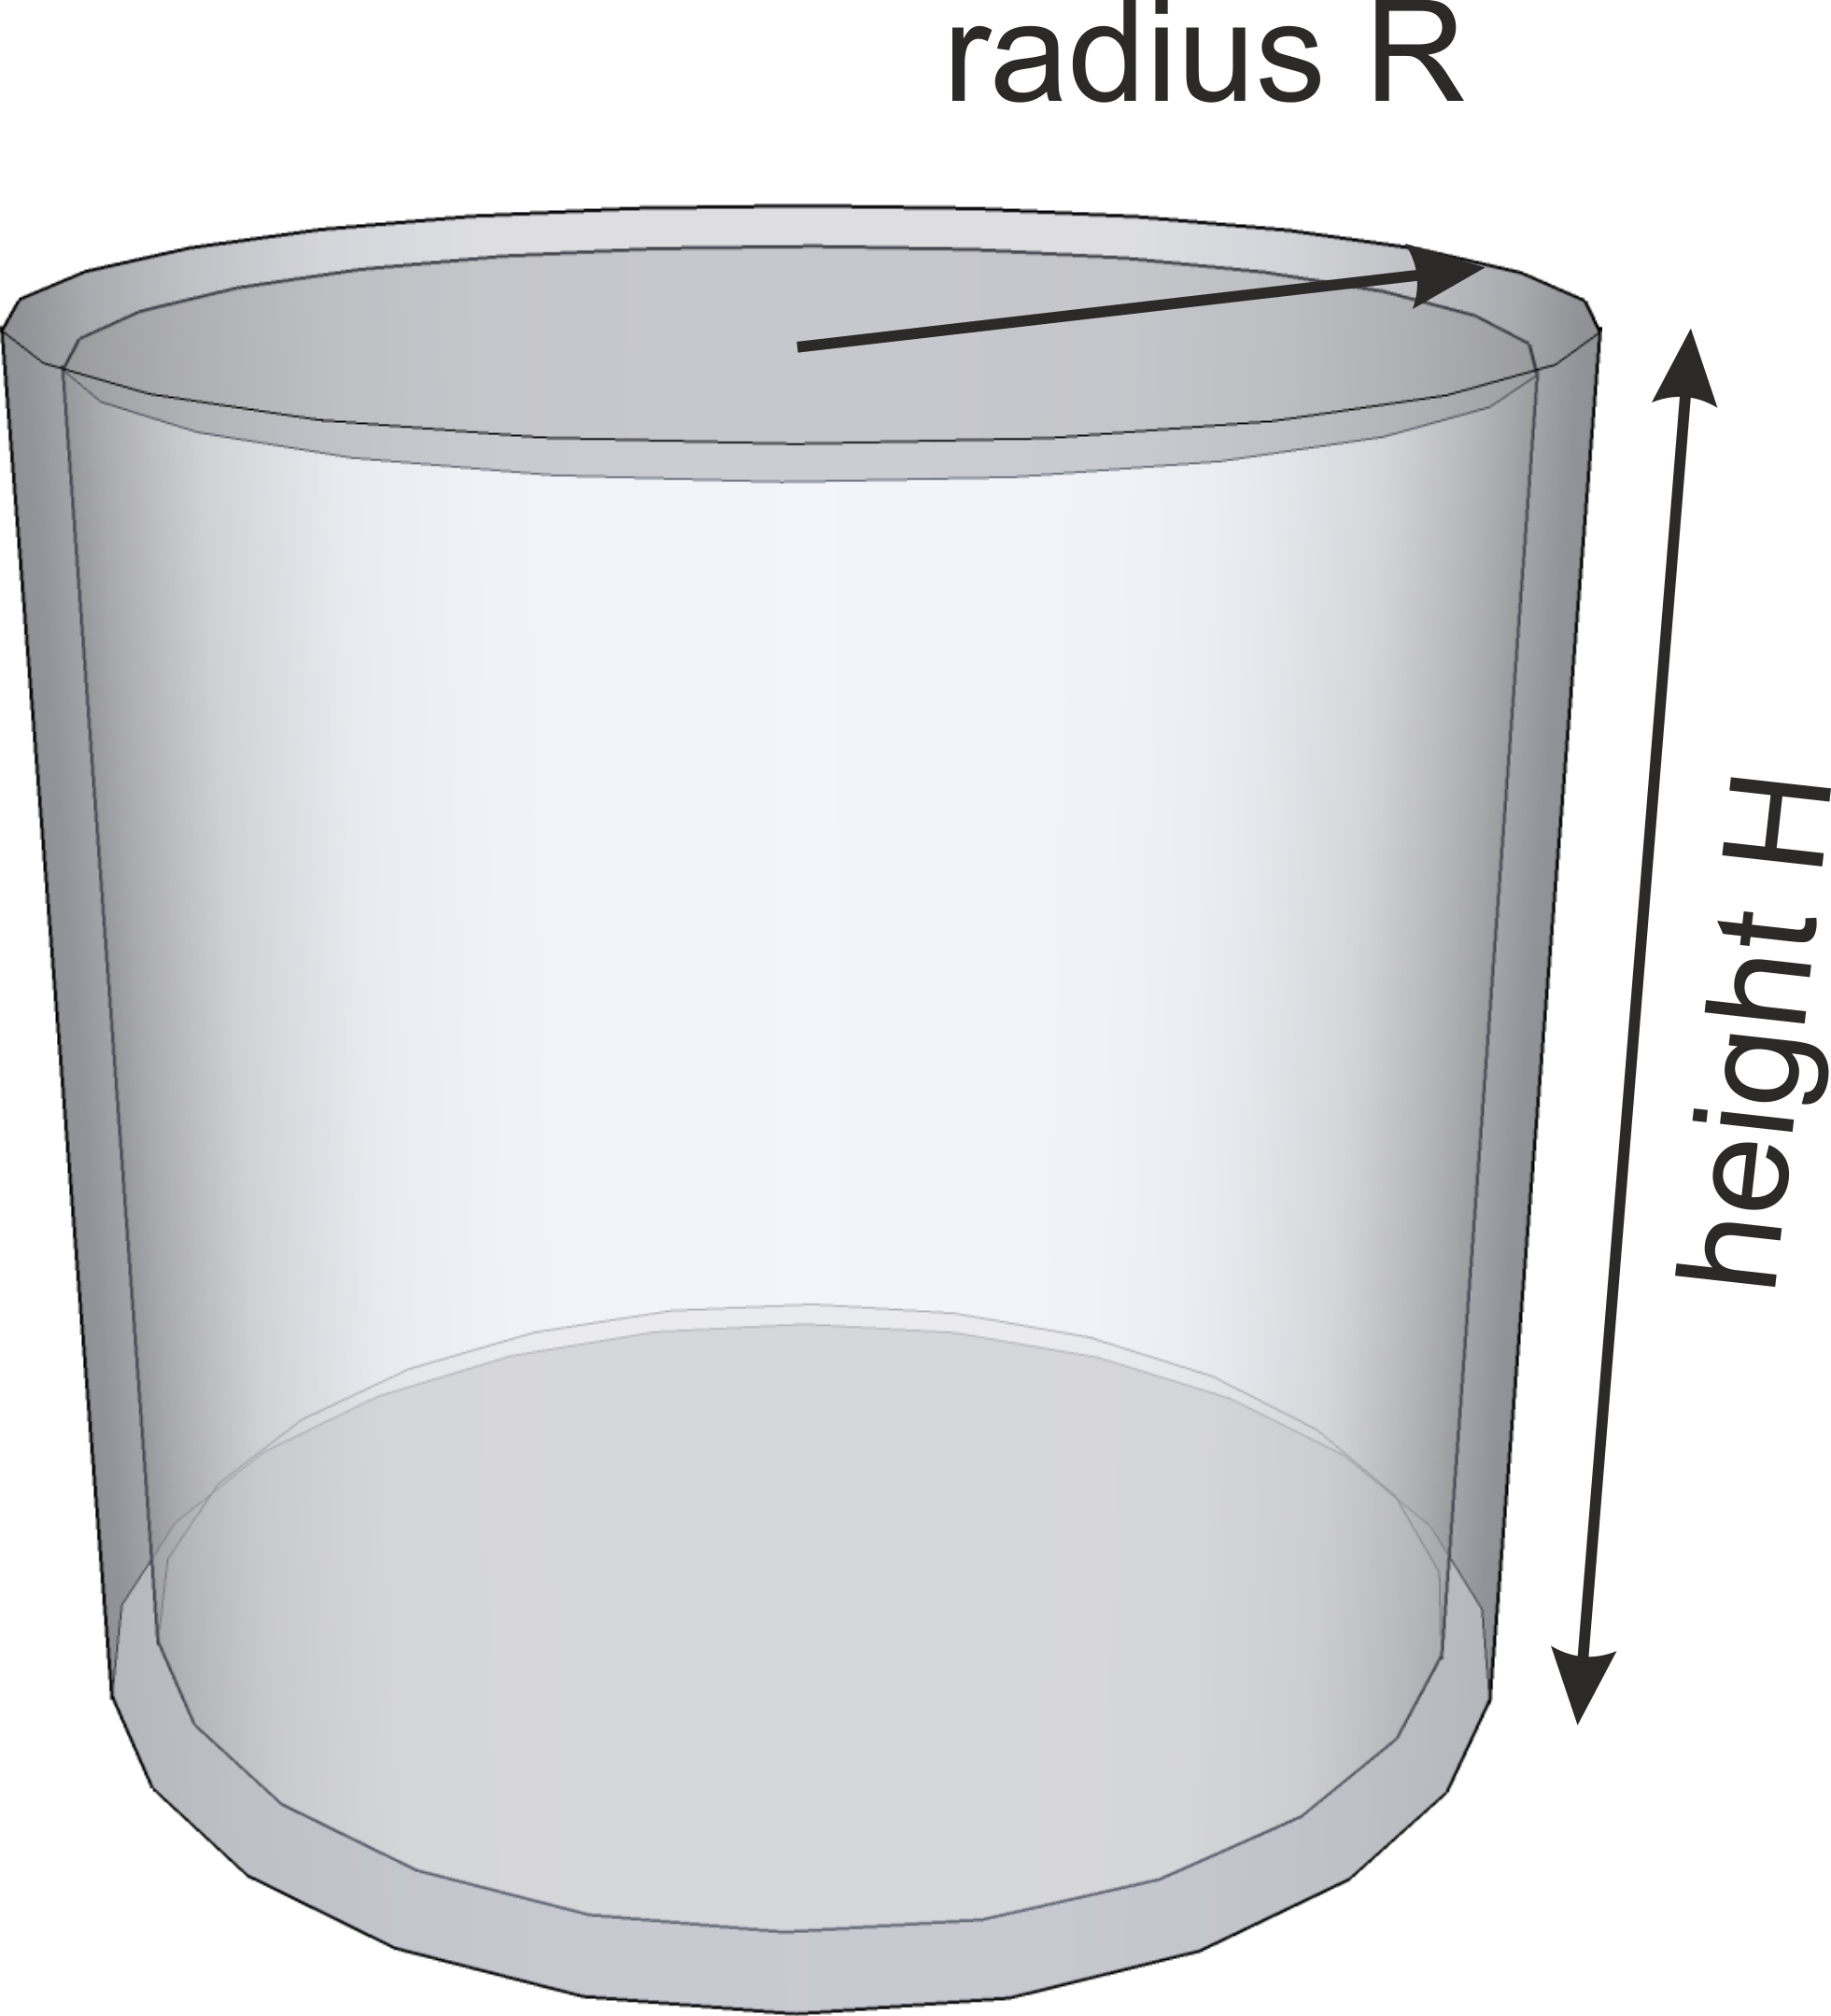
\includegraphics[width=0.3922\textwidth,height=0.4318\textwidth]{../images/form_factor/anisotropic/ThinHollowCylinder.png}
\end{center}
\caption{Sketch of a thin hollow cylinder of height $H$ and radius $R$. The thickness of the wall is assumed to be much smaller than the outer dimensions of the cylinder.}
\label{fig:ThinHollowCylinder}
\end{figure}

\begin{align}
\begin{split}
\Xi(Q,R,H,\alpha) & = 2\pi R
\left[ R \frac{J_1\left(Q R \sin\alpha\right)}{Q R \sin\alpha} \right. \\
& \left. \quad \quad + H J_0\left( \frac{QH}{2} \cos\alpha\right)\frac{\sin\left(\frac{QH}{2} \cos\alpha\right)}{\frac{QH}{2} \cos\alpha} \right]
\end{split} \\
P_\text{thc}(Q,R,H) &= \int_0^{\pi/2} \Xi^2(Q,R,H,\alpha) \sin\alpha \mathrm{d}\alpha \\
\begin{split}
P'_{thc}(Q,R,H) &= \int_0^\infty \int_0^\infty
\mathrm{LogNorm}(r,1,\sigma_R,1,R,1) \\
& \qquad \qquad  \mathrm{LogNorm}(h,1,\sigma_H,1,H,1) P_\text{thc}(Q,r,h)
\, \mathrm{d}h \, \mathrm{d}r
\end{split}
\label{eq:PprimeThinWalledCylinder_closed}
\end{align}

\vspace{5mm}

\hspace{1pt}\\
\underline{Input parameters for \texttt{P'(Q): Thin Hollow Cylinder}:}
\begin{description}
    \item[\texttt{R}] most probable cylinder radius $R$
    \item[\texttt{H}] most probable cylinder height $H$
    \item[\texttt{sima\_R}] width $\sigma_R$ of radius distribution (LogNorm)
    \item[\texttt{sima\_H}] width $\sigma_H$ of height distribution (LogNorm)
\end{description}

\noindent
\underline{Note}
\begin{itemize}
  \item This structure factor is supposed to be combined with a form factor of local planar objects which are implemented as form factor plugins
under "\texttt{[by plugin|thin obj.|Pcs(Q): local planar obj.]}".
\item The structure factor already has a log-normal width distribution for one parameter included.
\end{itemize}

\begin{figure}[htb]
\begin{center}
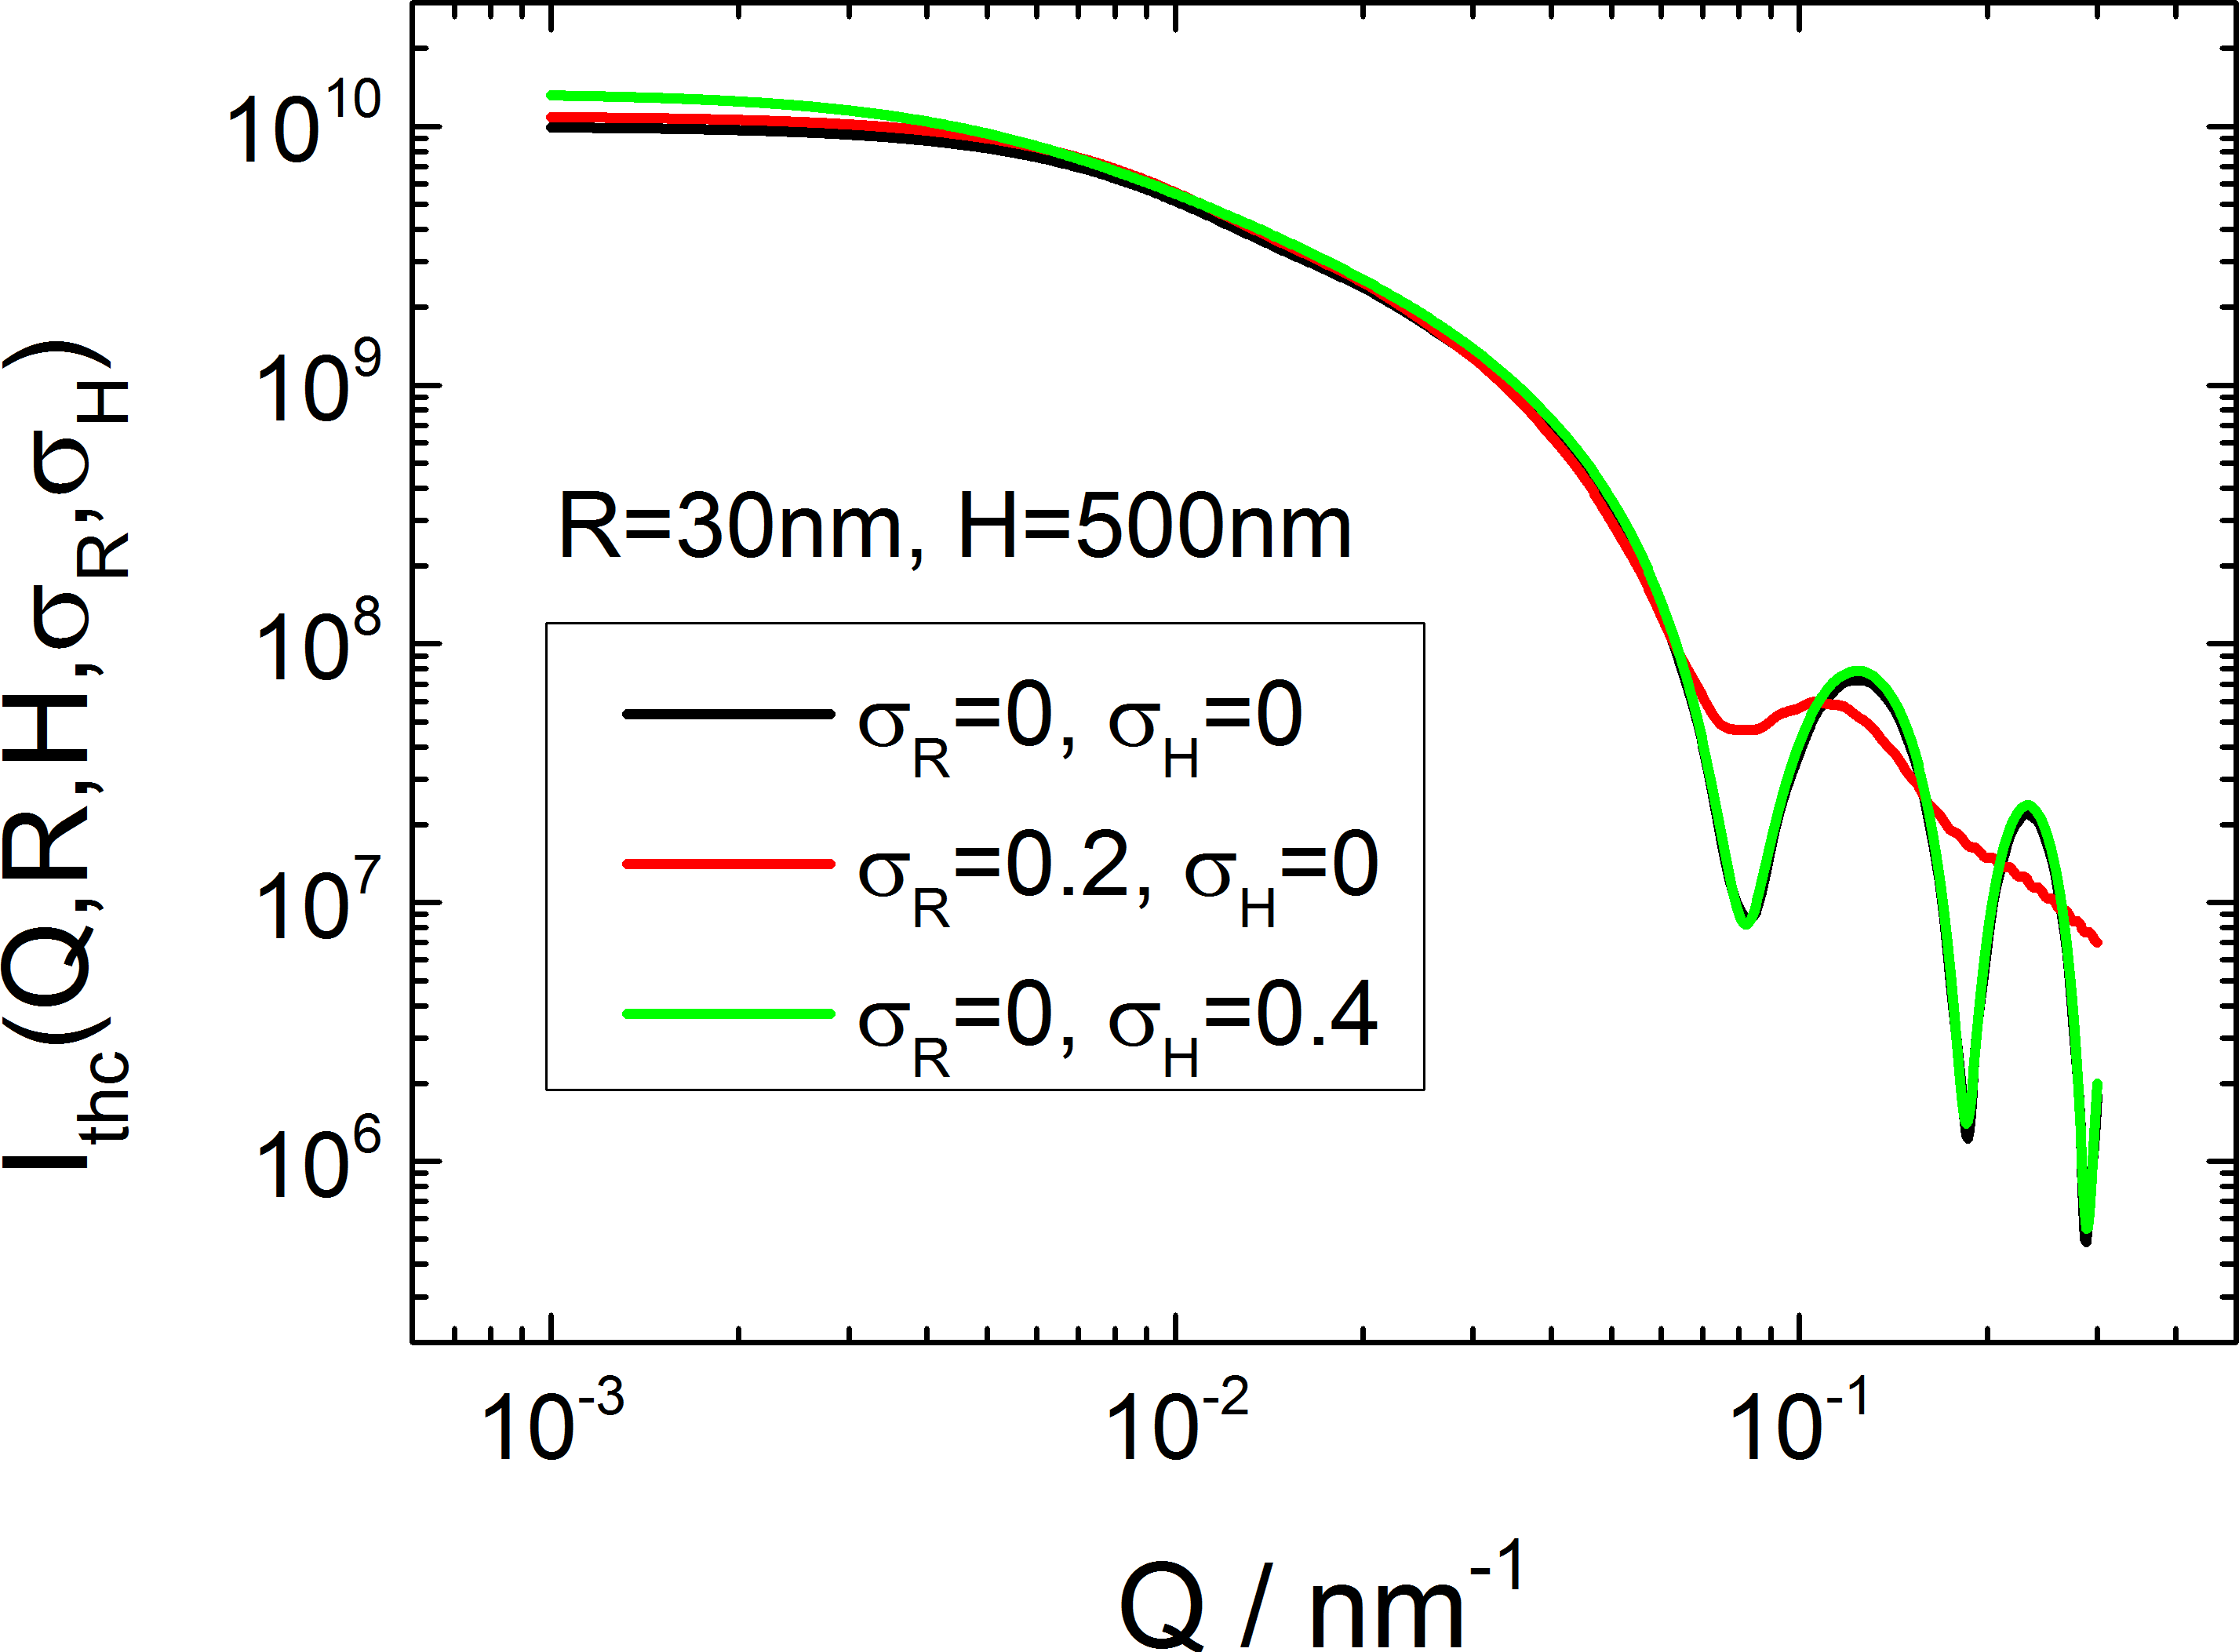
\includegraphics[width=0.8\textwidth,height=0.55\textwidth]{../images/form_factor/anisotropic/PprimeThinHollowCylinder.png}
\end{center}
\caption{Scattering curve for the structure factor "\texttt{P'(Q): Thin Hollow Cylinder}" in combination with a constant background of 1".}
\label{fig_IQ:PprimeThinHollowCylinder}
\end{figure}


\clearpage
\subsection{P'(Q) for local cylindrical obj.} ~\\
\label{plugin:Pprime4cylindrical}
\begin{enumerate}
\item thin rigid rod
\item wormlike structure
\end{enumerate}

\clearpage
\subsubsection{P'(Q): Rod} ~\\
\label{plugin:Pprime4rods}

\begin{figure}[htb]
\begin{center}
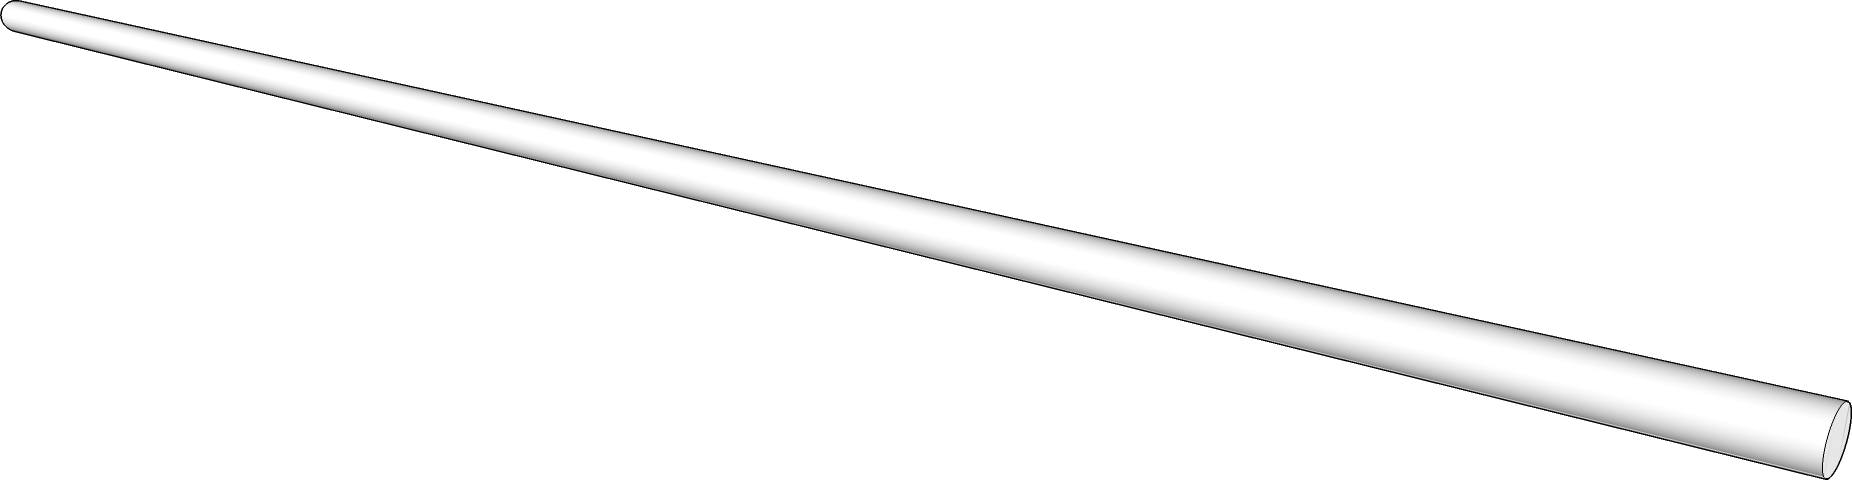
\includegraphics[width=0.926\textwidth,height=0.24\textwidth]{../images/form_factor/anisotropic/ThinRod.png}
\end{center}
\caption{Sketch of a thin Rod of Length $L$. The diameter of the rod is assumed to be much smaller than its length.}
\label{fig:ThinRod}
\end{figure}

\begin{align}
P'(Q) &= \int_0^\infty L'^2 \mathrm{LogNorm}(L',\sigma_L,1,L) \left(2 \frac{\mathrm{Si}(QL')}{QL'}-\frac{\sin^2(QL'/2)}{(QL'/2)^2} \right)\, \mathrm{d}L'
\label{eq:PprimeRod}
\end{align}
where $\mathrm{Si}(z)=\int_0^z\frac{\sin t}{t} \mathrm{d}t$ is the sine integral.

\vspace{5mm}

\hspace{1pt}\\
\underline{Input Parameters for model \texttt{P'(Q): Rod}:}\\
\begin{description}
\item[\texttt{L}]most probable length $L$ of rod
\item[\texttt{sigma\_L}] width LogNorm length distribution $\sigma_L$
\end{description}

\noindent
\underline{Note}
\begin{itemize}
  \item This structure factor is supposed to be combined with a form factor with local cylindrical geometry which are implemented as form factor plugins
under "\texttt{[by plugin|thin obj.|Pcs(Q): local cylindrical obj.]}".
\item The structure factor already has a log-normal width distribution for one parameter included.
\end{itemize}


\begin{figure}[htb]
\begin{center}
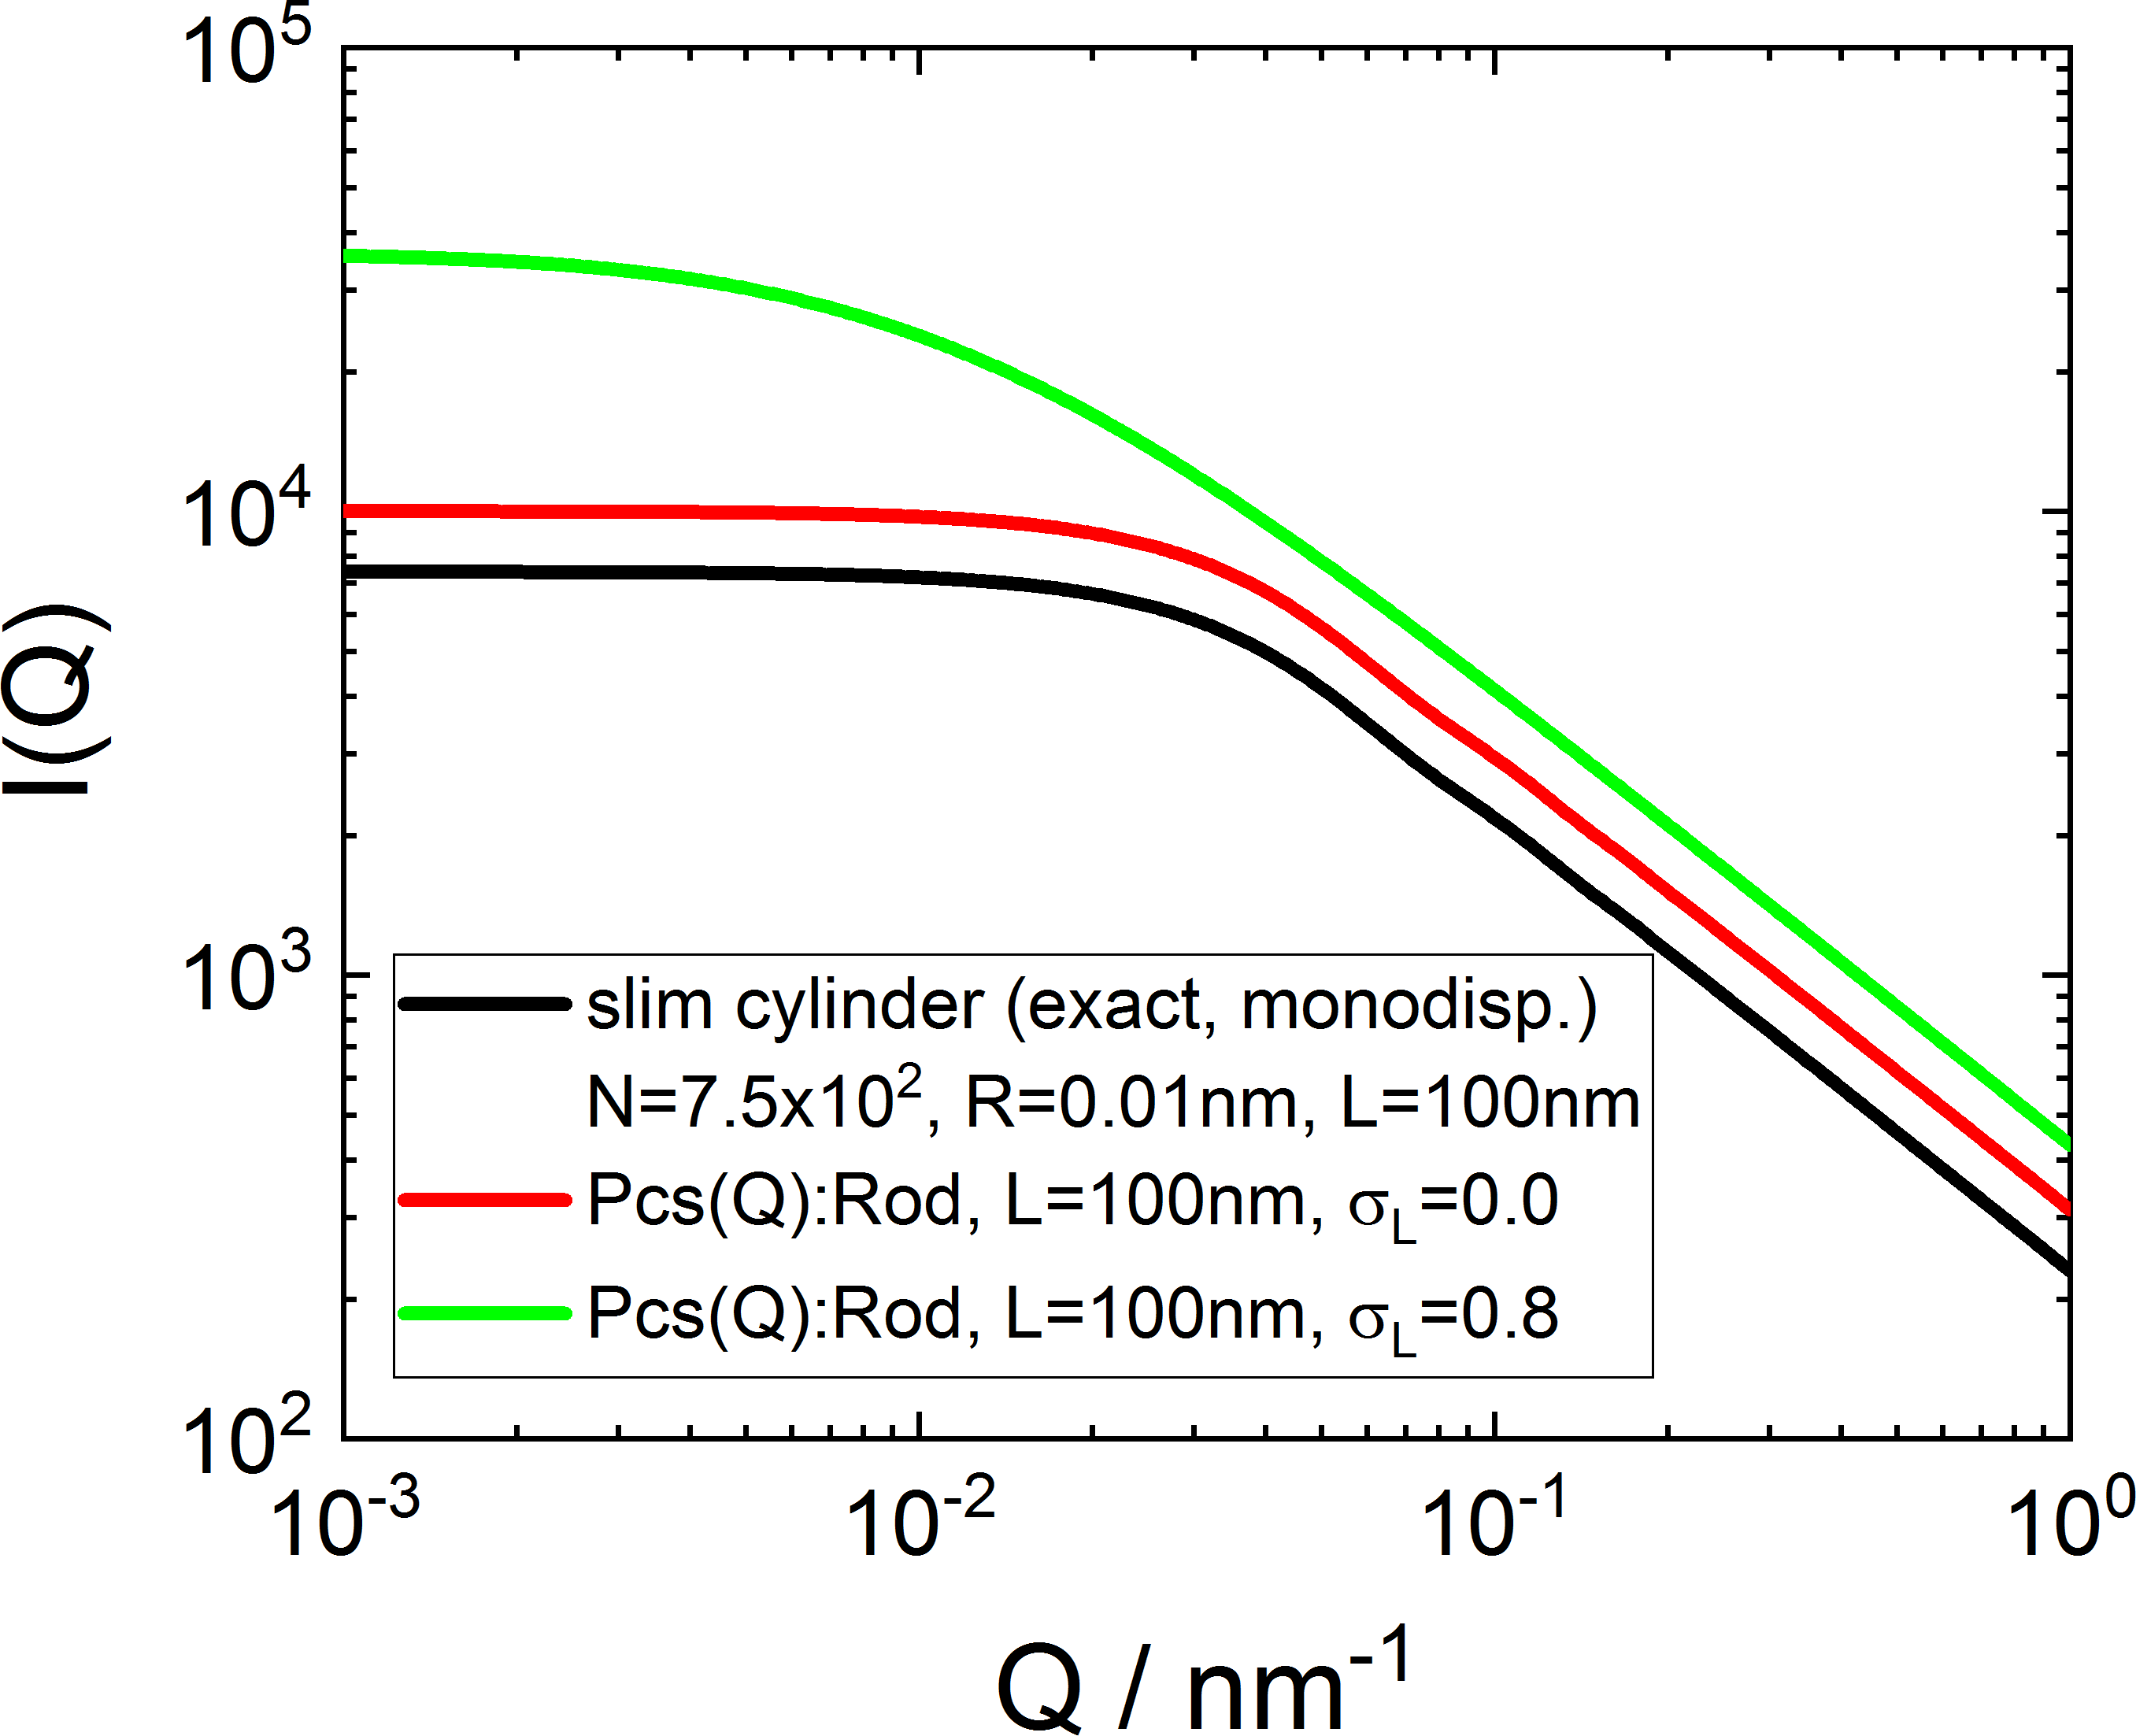
\includegraphics[width=0.8\textwidth,height=0.55\textwidth]{../images/form_factor/anisotropic/PprimeRod.png}
\end{center}
\caption{Scattering curve for the structure factor "\texttt{P'(Q): Rod}" in combination with a constant background of 1".}
\label{fig_IQ:PprimeRod}
\end{figure}

\clearpage
\subsubsection{P'(Q): freely joined chain of rods} ~\\
\label{plugin:Pprime4freelyjoinedchainofrods}

\begin{figure}[htb]
\begin{center}
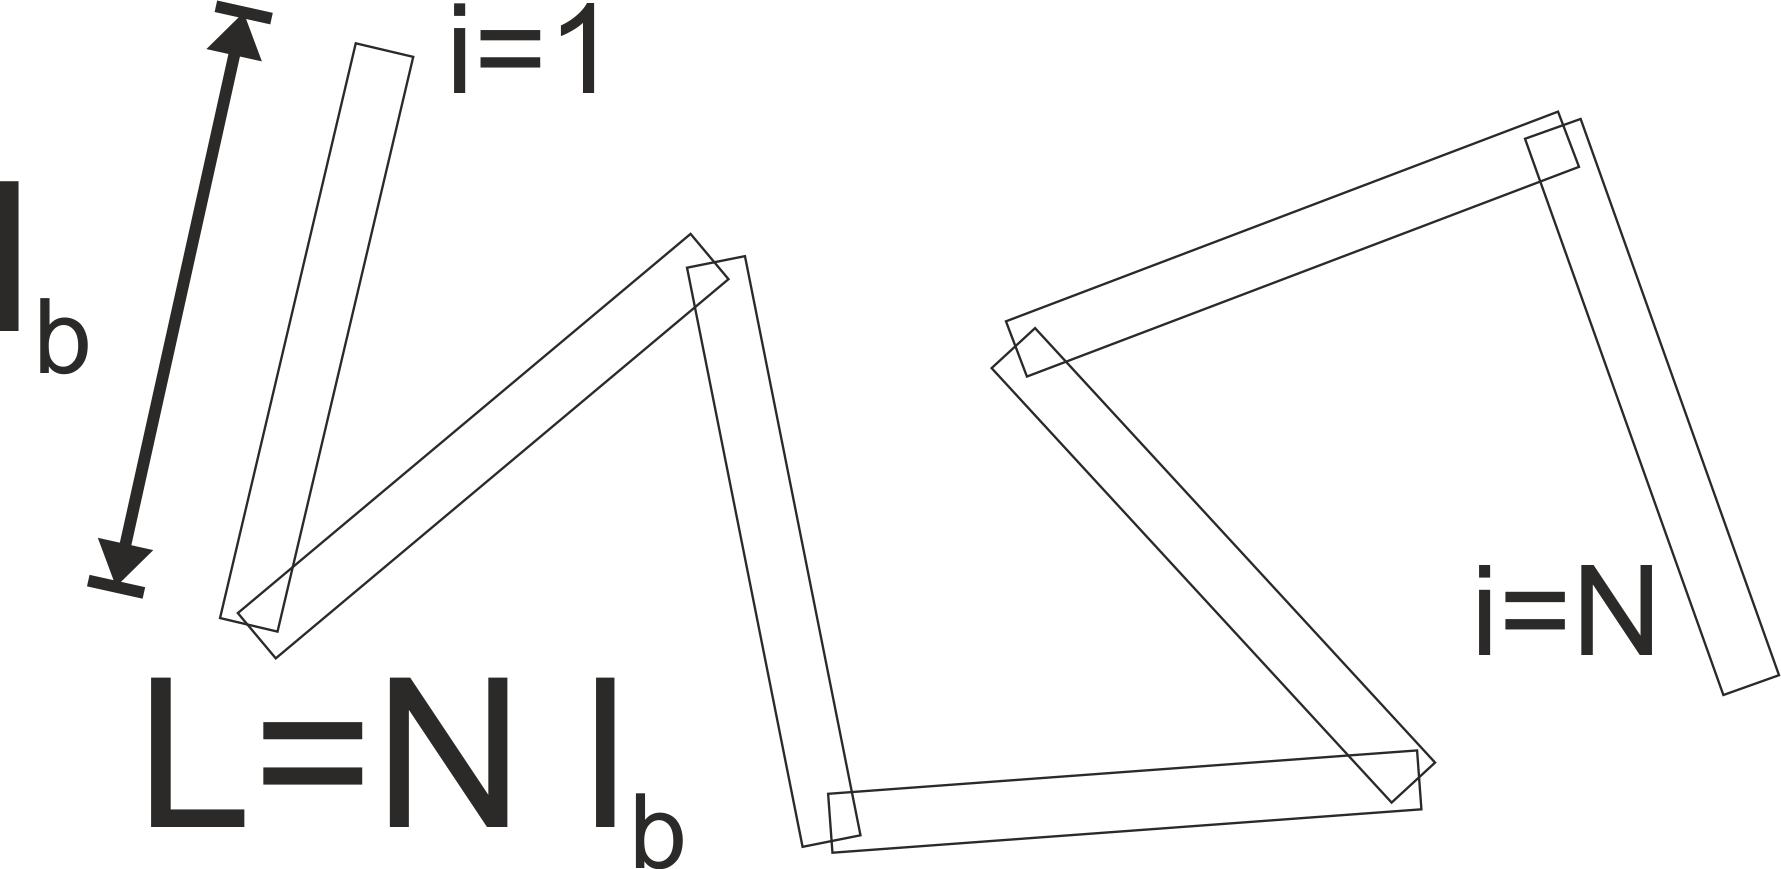
\includegraphics[width=0.75\textwidth]{freelyjoinedchainofrod.png}
\end{center}
\caption{Sketch of a freely joined chain of rods.}
\label{fig:freelyjoined chainofrod}
\end{figure}

This form factor describes a freely joined chain of infinitesimal thin rigid rods \cite{Hermans1958}.

\begin{align}
P'(Q,L,l_b) &= L^2\left( \frac{2l_b}{L}\left(\Lambda(\beta)-\frac12\left(\frac{\sin(\beta/2)}{\beta/2}\right)^2\right)\right) \\
&+L^2\Lambda^2(\beta)\left(\frac{2l_b}{L}\frac{1}{1-\gamma}-\frac{2l_b^2}{L^2}\frac{1-\gamma^{L/l_b}}{\left(1-\gamma\right)^2}\right) \nonumber \\
\beta &= q l_b \\
\gamma &= \frac{\sin(\beta)}{\beta} \\
\Lambda(\beta) &= \frac{\mathrm{Si}(\beta)}{\beta} \\
\mathrm{Si}(x) &= \int _{0}^{x}{\frac {\sin t}{t}}\,dt
\end{align}

\clearpage
\subsubsection{P'(Q): Koyama worm} ~\\
\label{plugin:Pprime4koyama}
\cite{Koyama1973,Koyama1974,Poetschke2000}
\begin{align}
P'(Q,L,l_b) &= L^2\frac{2}{X^2}\int_0^X (X-x)\phi(x)\mathrm{d}x \\
X &= \frac{2L}{l_b} \\
\phi(x) &= \exp\left(-\frac{s^2}{3}xf(x)\right) \frac{\sin(sxg(x))}{sxg(x)} \\
s &= \frac12 ql_b \\
xf(x) &= \frac{2\langle r^2\rangle}{l_b^2} - \frac12 x^2g^2(x) \\
x^2g^2(x) &= \frac{2\langle r^2\rangle}{l_b^2} \sqrt{10}\sqrt{1-\frac35 K} \\
K &= \frac{\langle r^4\rangle}{\langle r^2\rangle^2} \\
\langle r^2\rangle &= \frac{l_b^2}{2} \left(x-\left(1-e^{-x}\right)\right)\\
\langle r^4\rangle &= \frac{l_b^4}{4} \left\{\frac53 x^2 -\frac{52}{9}x-\frac{2}{27}\left(1-e^{-3x}\right)+8\left(1-e^{-x}\right)-2xe^{-x}\right\}
\end{align}

\clearpage
\subsubsection{P'(Q): Kholodenko's worm} ~\\
\label{plugin:Pprime4kohlodenko}

\begin{figure}[htb]
\begin{center}
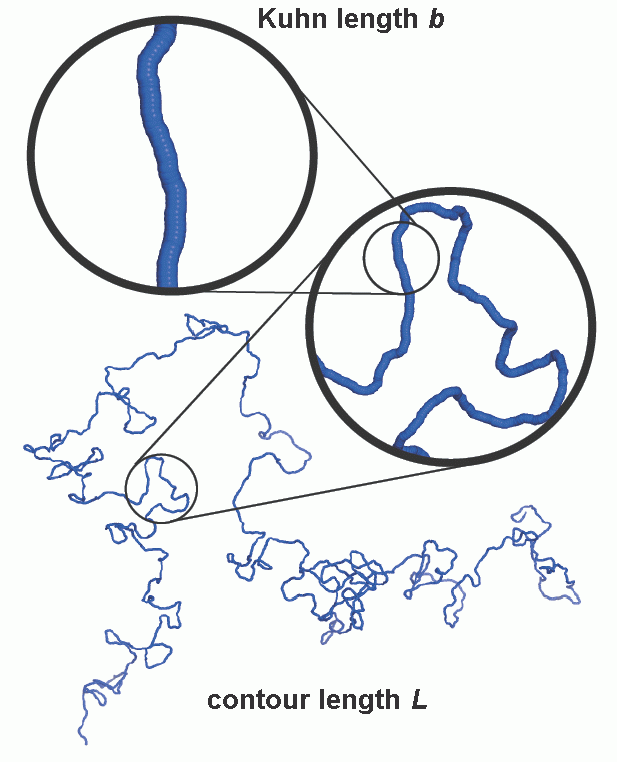
\includegraphics[width=0.617\textwidth,height=0.762\textwidth]{SemiflexiblePolymerTxt.png}
\end{center}
\caption{}
\label{fig:Pprime4KholodenkoWorm}
\end{figure}

By using the analogy between Dirac's fermions
and semi-flexible polymers
Kholodenko \cite{kholodenko93} could give a simple expression for the
scattering behaviour of wormlike structures. The form factor $P_0(Q)$ resulting
from Kholodenko's approach is designed to reproduce
correctly the rigid-rod limit and the random-coil limit.
Defining $x = 3L/l_b$ ($L$: contour length, $l_b$: Kuhn length), it is given by
\begin{align}
P_0(Q,L,l_b) &= \frac{2}{x} \left[I_{(1)} -\frac{1}{x}I_{(2)}\right]
\label{eq:KholodenkoPprime}
\end{align}
where
\begin{align}
I_{(n)}(x) &= \int_0^x  f(z) \, z^{n-1} \, dz
\end{align}
together with
\begin{align}
f(z) &=
\begin{cases} \displaystyle
\frac{1}{E}\frac{\sinh(Ez)}{\sinh(z)} & \text{for} \quad \displaystyle Q \leq \frac{3}{l_b}\\ \\
\displaystyle
\frac{1}{F}\frac{\sin(Fz)}{\sinh(z)} & \text{for} \quad \displaystyle Q > \frac{3}{l_b}
\end{cases}
\end{align}
and
\begin{align}
E = \sqrt{1-\left(\frac{l_bQ}{3}\right)^2} \quad \text{and} \quad F = \sqrt{\left(\frac{l_bQ}{3}\right)^2-1}
\end{align}

\vspace{5mm}

\hspace{1pt}\\
\underline{Input Parameters for model \texttt{P'(Q) Kholodenko Worm}:}\\
\begin{description}
\item[\texttt{lb}] Kuhn length\footnote{The Kuhn length $l_b$ is related to the length $a$ of
    locally stiff segment simply via $l_b=2a$} $l_B$ of semi-flexible worm-like structure
\item[\texttt{L}] contour length $L$ of semi-flexible worm-like structure
\end{description}

\noindent
\underline{Note}
\begin{itemize}
  \item This structure factor is supposed to be combined with a form factor with local cylindrical geometry which are implemented as form factor plugins
under "\texttt{[by plugin|thin obj.|Pcs(Q): local cylindrical obj.]}".
\item The equivalent solution of J.S. Pedersen \cite{Pedersen96Macrom} would be the expressions of wormlike structures without excluded volume effects.
\end{itemize}

\clearpage
\subsubsection{P'(Q): wormlike PS1} ~\\
\label{plugin:Pprime4wormPS1}

For worm-like micelles J.S. Pedersen \cite{Pedersen96Macrom} has developed three models, from which one is basing on a method developed by Yoshizaki et al.\ \cite{Yoshizaki1980}. This first version has been developed both with and without excluded volume effects.

~\\
\paragraph*{\textbf{Without Excluded Volume Effects.}}~\\

This first of the three solutions given by J.S. Pedersen \cite{Pedersen96Macrom} for
worm-like micelles starts from the expression for the scattering function as follows:
\begin{align}
\label{eq:SWC}
\begin{split}
S_\text{WC}(Q,L,l_B) &= L^2 \left[  \left(1-\chi(Q,L,l_B)\right)
            S_\text{chain}(Q,L,l_B) \right. \\
&  \left. \qquad  \qquad  +\chi(Q,L,l_B) S_\text{rod}(Q,L)    \right] \Gamma(Q,L,l_B)
\end{split}
\end{align}
where $S_\text{chain}(Q,L,l_B)$ is the scattering function of a flexible
chain without excluded volume effects and $S_\text{rod}(Q,L)$ is
the scattering function of a rod. Furthermore, $\chi(Q,L,l_b)$
is a crossover function, and the function $\Gamma(q,L,b)$ corrects
the crossover region.
The function $S_\text{chain}(Q,L,l_B)$ is given by the Debye function:
\begin{align}
\label{eq:SDebye}
S_\text{chain}(Q,L,l_B) &= S_\text{Debye}(Q,L,l_B) = 2\left[\exp(-u)+u-1\right]/u^2
\end{align}
with $u=\left\langle R_g^2\right\rangle_0 Q^2 $, where $\left\langle R_g^2\right\rangle_0$
is the ensemble average of the square of the radius of gyration and given by
\begin{align}
\left\langle R_g^2\right\rangle_0 &= \frac{Ll_B}{6}\left[1
        -\frac{3}{2n_B}
        +\frac{3}{2n_B^2}
        -\frac{3}{4n_B^3}
        \left[1-\exp(-2n_B)\right]\right]
\end{align}
where $n_B=L/l_B$ b is the number of statistical segments of the chain.
The function $S\text{rod}(Q,L)$ in \ref{eq:SWC} is the scattering function
of an infinitely thin rod
\begin{align}
S_\text{rod}(Q,L) &= 2 \text{Si}(Q,L)/(QL)-4\sin^2(QL/2)/(QL)^2
\end{align}
where
\begin{align}
\text{Si}(Q,L) &= \int_0^x t^{-1} \sin t \; \mathrm{d}t
\end{align}
Furthermore we have
\begin{align}
\chi(Q,L,l_B) &= \exp\left(-\xi^{-5}\right)
\end{align}
The parameter $\xi$ is given by
\begin{align}
\xi &= Q\frac{\pi}{2L} \left\langle R_g^2\right\rangle_0
\end{align}
The function $\Gamma(Q,L,l_B)$ is given by
\begin{align}
\Gamma(Q,L,l_B) &= 1+(1-\chi)\sum_{i=2}^5A_i\xi^i + \chi\sum_{i=0}^2B_i\xi^{-i}
\end{align}
where
\begin{align}
\begin{split}
A_i &= \sum_{j=0}^2a_1(i,j) \left(\frac{L}{l_B}\right)^{-j} \exp(-10 l_B/L) \\
& \qquad \qquad + \sum_{j=1}^2a_2(i,j) \left(\frac{L}{l_B}\right)^{j} \exp(-2 L/l_B)
\end{split}
\end{align}
and
\begin{align}
\begin{split}
B_i & = \sum_{j=0}^2b_1(i,j) \left(\frac{L}{l_B}\right)^{-j} \\
    & \qquad \qquad + \sum_{j=1}^2b_2(i,j) \left(\frac{L}{l_B}\right)^{j} \exp(-2 L/l_B)
\end{split}
\end{align}
The values of $a_1(i,j), a_2(i,j), b_1(i,j)$, and $b_2(i,j)$ are listed in table \ref{table:numValWMPS1noexv}
\begin{table}
  \caption{Values for the parameters in the numerical expressions for the scattering function for worm-like chains \textbf{without} excluded volume effects \cite{Pedersen96Macrom}}
  \label{table:numValWMPS1noexv}
  \centering
  \begin{tabular}{l c|l c|l c|l c}
     \hline
     % after \\: \hline or \cline{col1-col2} \cline{col3-col4} ...
               &          &           &          & $b_1(0,0)$ & -0.0162  &            &          \\
               &          &           &          & $b_1(1,0)$ &  0.09046 &            &          \\
     $a1(2,0)$ &  0.3054  &           &          & $b_1(2,0)$ &  0.1213  &            &          \\
     $a1(3,0)$ &  0.05777 &           &          &            &          &            &          \\
     $a1(4,0)$ & -0.00604 &           &          &            &          &            &          \\
     $a1(5,0)$ & -0.03902 &           &          &            &          &            &          \\
               &          &           &          & $b_1(0,1)$ & -0.3565  & $b_2(0,1)$ & -0.3946  \\
               &          &           &          & $b_1(1,1)$ &  0.1909  & $b_2(1,1)$ & -0.2231  \\
     $a1(2,1)$ &  0.2316  & $a2(2,1)$ & -0.4963  & $b_1(2,1)$ &  0.15634 & $b_2(2,1)$ & -0.2546  \\
     $a1(3,1)$ &  0.26531 & $a2(3,1)$ &  0.03688 &            &          &            &          \\
     $a1(4,1)$ &  0.3706  & $a2(4,1)$ &  0.30570 &            &          &            &          \\
     $a1(5,1)$ & -1.0081  & $a2(5,1)$ &  0.39013 &            &          &            &          \\
               &          &           &          & $b_1(0,2)$ & -0.3078	 & $b_2(0,2)$ &  1.1361  \\
               &          &           &          & $b_1(1,2)$ &  0.05176 & $b_2(1,2)$ & -0.01615 \\
     $a1(2,2)$ & -22.779  & $a2(2,2)$ & -0.4678  & $b_1(2,2)$ &  0.01568 & $b_2(2,2)$ & -0.07606 \\
     $a1(3,2)$ &  23.2457 & $a2(3,2)$ &  0.3365  &            &          &            &          \\
     $a1(4,2)$ &  8.1092  & $a2(4,2)$ &  0.4290  &            &          &            &          \\
     $a1(5,2)$ & -3.3603  & $a1(5,2)$ &  0.3737  &            &          &            &          \\
     \hline
   \end{tabular}
\end{table}

\clearpage
\paragraph*{\textbf{With Excluded Volume Effects.}}~\\

To include excluded volume effects in eq.\ \ref{eq:SWC} the function for a flexible chain $S_\text{chain}(Q,L,l_B)$ needs to be replaced by one with excluded volume effects included
\begin{align}
\label{eq:exvSWC}
\begin{split}
S_\text{WC}(Q,L,l_B) &= L^2 \left[  \left(1-\chi(Q,L,l_B)\right)
            S_\text{exv}(Q,L,l_B) \right. \\
&  \left. \qquad  \qquad  +\chi(Q,L,l_B) S_\text{rod}(Q,L)    \right] \Gamma(Q,L,l_B)
\end{split}
\end{align}
The scattering of a chain with excluded volume effects is given by
\begin{multline}
S_\text{exv}(Q,L,l_B) = w(Q,R_g) S_\text{Debye}(Q,L,l_B) + \\
 \left[1-w(q R_g)\right[\left[C_1\left(QR_g\right)^{-1/\nu}
                                           + C_2\left(QR_g\right)^{-2/\nu}
                                           + C_3\left(QR_g\right)^{-3/\nu}\right]
\end{multline}
where $S_\text{Debye}(Q,L,l_B)$ is given by eq.\ \ref{eq:SDebye} and
\begin{align}
R_g^2&=\alpha(L/l_B)^2 \langle R_g^2\rangle^2
\label{eq:RgexvWC}
\end{align}
with $\alpha(L/l_B)$ being an expansion factor following the expression:
\begin{align}
\alpha(x)^2 &= \left[ 1+(x/3.12)^2+(x/8.67)^3 \right]^{\epsilon/3}
\end{align}
and $\epsilon=0.170$. The function $w(x)$ is another emical cross-over function chosen as:
\begin{align}
w(x) &= \left[ 1+\tanh\left(\frac{x-C_4}{C_5}\right)/C_5 \right]/2
\end{align}
The parameters $C_i$ have been given in \cite{Pedersen96Macrom} as
$C_1=1.220$, $C_2=0.4288$, $C_3=-1.651$, $C_4=1.523$, and $C_5=0.1477$.

Furthermore the parameter $\xi$ in the cross-over function $\chi(Q,L,l_B)$ needs to be chosen as
\begin{align}
\xi&=Ql_B\left(\frac{\pi l_B}{1.103 L}\right)^{3/2}\left[\frac{R_g^2}{l_B^2}\right]^{1.282}
\end{align}
with $R_g^2$ defined in eq.\ \ref{eq:RgexvWC}. Last, but not least the values of $a_1(i,j), a_2(i,j), b_1(i,j)$, and $b_2(i,j)$ need to be taken from table \ref{table:numValWMPS1withexv}.
\begin{table}
  \caption{Values for the parameters in the numerical expressions for the scattering function for worm-like chains \textbf{with} excluded volume effects \cite{Pedersen96Macrom}}
  \label{table:numValWMPS1withexv}
  \centering
  \begin{tabular}{l c|l c|l c|l c}
     \hline
     % after \\: \hline or \cline{col1-col2} \cline{col3-col4} ...
               &          &           &          & $b_1(0,0)$ & -0.0699  &            &          \\
               &          &           &          & $b_1(1,0)$ & -0.0900  &            &          \\
     $a1(2,0)$ & -0.1222  &           &          & $b_1(2,0)$ &  0.2677  &            &          \\
     $a1(3,0)$ &  0.3051  &           &          &            &          &            &          \\
     $a1(4,0)$ & -0.0711  &           &          &            &          &            &          \\
     $a1(5,0)$ &  0.0584  &           &          &            &          &            &          \\
               &          &           &          & $b_1(0,1)$ &  0.1342  & $b_2(0,1)$ & -0.5171  \\
               &          &           &          & $b_1(1,1)$ &  0.0138  & $b_2(1,1)$ & -0.2028  \\
     $a1(2,1)$ &  1.761   & $a2(2,1)$ &  0.1212  & $b_1(2,1)$ &  0.1898  & $b_2(2,1)$ & -0.3112  \\
     $a1(3,1)$ &  2.252   & $a2(3,1)$ & -0.4169  &            &          &            &          \\
     $a1(4,1)$ & -1.291   & $a2(4,1)$ &  0.1988  &            &          &            &          \\
     $a1(5,1)$ &  0.6994  & $a2(5,1)$ &  0.3435  &            &          &            &          \\
               &          &           &          & $b_1(0,2)$ & -0.2020	 & $b_2(0,2)$ &  0.6950  \\
               &          &           &          & $b_1(1,2)$ & -0.0114  & $b_2(1,2)$ & -0.3238  \\
     $a1(2,2)$ & -26.04   & $a2(2,2)$ &  0.0170  & $b_1(2,2)$ &  0.0123  & $b_2(2,2)$ & -0.5403  \\
     $a1(3,2)$ &  20.00   & $a2(3,2)$ & -0.4731  &            &          &            &          \\
     $a1(4,2)$ &  4.382   & $a2(4,2)$ &  0.1869  &            &          &            &          \\
     $a1(5,2)$ &  1.594   & $a1(5,2)$ &  0.3350  &            &          &            &          \\
     \hline
   \end{tabular}
\end{table}


\vspace{5mm}

\hspace{1pt}\\
\underline{Input Parameters for model \texttt{P'(Q) Worm(PS1)} (with excluded volume effects):}\\
\begin{description}
\item[\texttt{lb}] Kuhn length\footnote{The Kuhn length $l_b$ is related to the length $a$ of
    locally stiff segment simply via $l_b=2a$} $l_B$ of semi-flexible worm-like structure
\item[\texttt{L}] contour length $L$ of semi-flexible worm-like structure
\item[\texttt{exvol}] input flag to select the variant with or without excluded volume effects: $\mathrm{exvol} \geq 1$ with excluded volume effects, $\mathrm{exvol} < 1$ without excluded volume effects
\end{description}

\noindent
\underline{Note}
\begin{itemize}
  \item This structure factor is supposed to be combined with a form factor with local cylindrical geometry which are implemented as form factor plugins
under "\texttt{[by plugin|thin obj.|Pcs(Q): local cylindrical obj.]}".
\end{itemize}

\clearpage
\subsubsection{P'(Q): wormlike PS2} ~\\
\label{plugin:Pprime4wormPS2}
For this version of the wormlike structure \cite{Pedersen96Macrom} parameterized the structure factor in one for long and short wormlike micelles depending on their ratio $n_b=\frac{L}{l_B}$ is larger or smaller than 2.
\begin{align}
S_\mathrm{PS2}(Q,L,l_B) &=
\begin{cases}
    S_\mathrm{SB}(Q,L,l_B) f_1 + S_\mathrm{loc}(Q,L,1) (1-f_1) & \mbox{ for~}  n_b > 2 \\
    S_\mathrm{Debye}(Q,Q^2\langle R_g^2\rangle_0) f_2 + S_\mathrm{loc}(Q,L,l_B,a_1) (1-f_2) & \mbox{ for~}  n_b \leq 2
\end{cases}
\end{align}
with $\langle R_g^2\rangle_0 = Ll_B/6\left(1-\frac{3}{2 n_b}
            +\frac{3}{2 n_b^2}
			-\frac{3}{4 n_b^3}
			\left[1-\exp(-2 n_b)\right]\right)$.
The transition functions are defined as
\begin{align}
f_1 &= \exp\left[-\left(\frac{Ql_B}{q_1}\right)^{p_1}\right] \\
f_2 &= \exp\left[-\left(\frac{Ql_B}{q_2}\right)^{p_2}\right]
\end{align}
The Debye function is given by
\begin{align}
S_\mathrm{Debye}(Q,u) &= 2\left[\exp(-u)+u-1\right]/u^2
\end{align}
For large wormlike micelles in the small $Q$ region the scattering function calculated for the
Daniels approximation \cite{Daniels1952} according to \cite{Sharp1968,Pedersen96Macrom} is
\begin{align}
S_\mathrm{SB}(Q,L,l_B) &= S_\mathrm{Debye}(Q,Q^2 R_g^2)+
    \frac{\left[\frac{4}{15} +\frac{7}{15u}-\left(\frac{11}{15}+\frac{7}{15u}\right)\exp(-u)\right]}{n_b}\\
R_G^2 &=Ll_B/6
\end{align}
and in the large $Q$ range
\begin{align}
S_\mathrm{loc}(Q,L,l_B,a_1) &= \frac{a_1}{Ll_BQ^2} + \frac{\pi}{LQ}
\end{align}
The optimized values of the parameters $q_1,p_1, a_1, a_2, q_2$, and $ p_2$ are
$q_1 = 5.53$, $p_1 = 5.33$, $a_1 = 0.0625$, $a_2 = 11.7$, $p_2 = 3.95$ and
$q_2 = a_2/n_b$.

\vspace{5mm}

\hspace{1pt}\\
\underline{Input Parameters for model \texttt{P'(Q) Worm(PS2)} (always without excluded volume effects):}\\
\begin{description}
\item[\texttt{lb}] Kuhn length\footnote{The Kuhn length $l_b$ is related to the length $a$ of
    locally stiff segment simply via $l_b=2a$} $l_B$ of semi-flexible worm-like structure
\item[\texttt{L}] contour length $L$ of semi-flexible worm-like structure
\end{description}

\noindent
\underline{Note}
\begin{itemize}
  \item This structure factor is supposed to be combined with a form factor with local cylindrical geometry which are implemented as form factor plugins
under "\texttt{[by plugin|thin obj.|Pcs(Q): local cylindrical obj.]}".
\end{itemize}


\clearpage
\subsubsection{P'(Q): wormlike PS3} ~\\
\label{plugin:Pprime4wormPS3}

This version of the wormlike structure model originally from \cite{Pedersen96Macrom} is implemented together with the suggestions for corrections given in \cite{Chen2006}.
\begin{align}
q_0 &=
\begin{cases}
3.1 & \mbox{for~} L>4l_B \\
\max\left\{a_3 l_B/R_G,4\right\} & \mbox{for~} L\leq 4l_B \wedge \mbox{without excl. vol.}\\
\max\left\{a_3 l_B/R_G,3\right\} & \mbox{for~} L\leq 4l_B \wedge \mbox{with excl. vol.}\\
\end{cases}\\
R_G^2 &=
\begin{cases}
\frac{Ll_B}{6} & \mbox{for~} L > 4l_B \wedge \mbox{without excl. vol.} \\
\frac{Ll_B}{6} f\left(\frac{L}{l_B}\right) & \mbox{for~} L > 4l_B \wedge \mbox{with excl. vol.} \\
\frac{Ll_B}{6} f\left(\frac{L}{l_B}\right)& \mbox{for~} L\leq 4l_B \wedge \mbox{without excl. vol.}\\
\frac{Ll_B}{6} f\left(\frac{L}{l_B}\right)\alpha^2\left(\frac{L}{l_B}\right) & \mbox{for~} L\leq 4l_B \wedge \mbox{with excl. vol.}\\
\end{cases} \\
f(x) &= 1-\frac{3}{2x}+\frac{3}{2\left(x\right)^2}-\frac{3}{4\left(x\right)^3}\left[1-\exp\left(-2x\right)\right]\\
\alpha(x) &= \left(1+(x/3.12)^2+(x/8.67)^3\right)^{\epsilon/3} \\
\epsilon&=0.170 \\
C\left(\frac{L}{l_B}\right) &=
\begin{cases}
a_4/\left(\frac{L}{l_B}\right)^{p_3} & \mbox{for~} L > 10l_B \wedge \mbox{with excl. vol.} \\
1 & \mbox{ otherwise}\\
\end{cases}
\end{align}
with  $a_3=2.02$, $a_4=3.06$, and $p_3=0.44$.
\begin{align}
S(Q,L,l_B) &=
\begin{cases}
L^2 S_{\textrm{small~} Q}(Q,L,l_B)& \mbox{for~}  Ql_B<q_0 \\
L^2 \left(\frac{a_1}{(Ql_B)^{p_1}}+\frac{a_2}{(Ql_B)^{p_2}}+\frac{\pi}{QL}\right)& \mbox{for~}  Ql_B\geq q_0  \\
\end{cases}\\
p_1 &=
\begin{cases}
4.95 & \mbox{for~} L > 4l_B \wedge \mbox{without excl. vol.} \\
5.13 & \mbox{for~} L \leq 4l_B \wedge \mbox{without excl. vol.} \\
4.12 & \mbox{for~} L > 4l_B \wedge \mbox{with excl. vol.} \\
5.36 & \mbox{for~} L \leq 4l_B \wedge \mbox{with excl. vol.} \\
\end{cases}\\
p_2 &=
\begin{cases}
5.29 & \mbox{for~} L > 4l_B \wedge \mbox{without excl. vol.} \\
7.47 & \mbox{for~} L \leq 4l_B \wedge \mbox{without excl. vol.} \\
4.42 & \mbox{for~} L > 4l_B \wedge \mbox{with excl. vol.} \\
5.62 & \mbox{for~} L \leq 4l_B \wedge \mbox{with excl. vol.} \\
\end{cases}
\end{align}
The parameters $a_1$ and $a_2$ are defined by the condition that for $Ql_B=q_0$ the small and large $Q$ region are continuous and smooth, i.e. that also the first derivative of $\mathrm{d}S(q,L,l_B)/\mathrm{d}q|_{q=q_0/l_B}$ is continuous.
\begin{align}
S_{\textrm{small~} Q}(Q,L,l_B) &=
\begin{cases}
 S_\textrm{SB}(Q,R_G)    & \mbox{for~} L >    4l_B   \\
 S_\textrm{Debye}(Q,R_G) & \mbox{for~} L \leq 4l_B  \wedge \mbox{without excl. vol.}\\
 S_\textrm{cexv}(Q,R_G)  & \mbox{for~} L \leq 4l_B  \wedge \mbox{with excl. vol.} \\
\end{cases}
\end{align}
where
\begin{align}
S_\textrm{SB}(Q,R_G) &= S_\mathrm{Debye}(Q,Q^2 R_g^2)+
    \frac{\left[\frac{4}{15} +\frac{7}{15u}-\left(\frac{11}{15}+\frac{7}{15u}\right)\exp(-u)\right]}{L/l_B}\\
S_\textrm{Debye}(Q,R_G) &= 2\left(\exp(-u)+u-1\right)/u^2\\
S_\textrm{cexv}(Q,R_G) &= S_\textrm{EXV}(Q,R_G)  +C\left(\frac{L}{l_B}\right)\frac{\frac{4}{15}+\frac{7}{15u}-\left(\frac{11}{15}+\frac{7}{15u}\right)\exp(-u)}{L/l_B} \\
u &= Q^2R_G^2 \\
x &= QR_G \\
S_\textrm{EXV}(Q,R_G) &= (1-w)S_\textrm{Debye}(Q,R_G) \\
&+ w f_\textrm{corr}(Q) \left(C_1x^{-1/\nu}+C_2x^{-2/\nu}+C_3x^{-3/\nu}\right) \nonumber \\
w &= \frac12\left(1+\tanh((x-1.523)/0.1477)\right)
\end{align}
with the optimized parameters $C_1 = 1.2220$, $C_2 = 0.4288$, and $C_3 = -1.651$.
As $S_\textrm{EXV}$ should be a monotonic decreasing function also at very small $Q$-values the correction factor $f_\textrm{corr}(Q,R_G)$ has been introduced by \cite{Chen2006}
\begin{align}
f_\textrm{corr}(Q,R_G) &=
\begin{cases}
1 & \mbox{for~} \frac{\mathrm{d}S_\textrm{cexv}(Q,R_G)}{\mathrm{d}Q} \leq 0\\
0 & \mbox{otherwise}
\end{cases}
\end{align}
\vspace{5mm}

\hspace{1pt}\\
\underline{Input Parameters for model \texttt{P'(Q) Worm(PS3)} (with/without excluded volume effects):}\\
\begin{description}
\item[\texttt{lb}] Kuhn length\footnote{The Kuhn length $l_b$ is related to the length $a$ of
    locally stiff segment simply via $l_b=2a$} $l_B$ of semi-flexible worm-like structure
\item[\texttt{L}] contour length $L$ of semi-flexible worm-like structure
\item[\texttt{exvol}] input flag to select the variant with or without excluded volume effects: $\mathrm{exvol} \geq 1$ with excluded volume effects, $\mathrm{exvol} < 1$ without excluded volume effects
\end{description}

\noindent
\underline{Note}
\begin{itemize}
  \item This structure factor is supposed to be combined with a form factor with local cylindrical geometry which are implemented as form factor plugins
under "\texttt{[by plugin|thin obj.|Pcs(Q): local cylindrical obj.]}".
\end{itemize}

\clearpage
\subsection{local planar  obj.} ~\\
\label{plugin:LocalPlanar)}
A few selected combinations of the cross-sections $P_\mathrm{cs}(Q)$ and shape factors $P'(Q)$ have been collected for thin planar objects in this subsection to give access to structure factor effects on these systems. The list can easily be extended on request.

\vspace{5mm}

\noindent
\subsubsection{Disc+SD+BiLayerGauss} ~\\

\noindent
In this form factor the cross section term of a lipid bilayer (eq.\ \ref{eq:PcsBilayer}) is combined with a shape factor of a disc (eq.\ \ref{eq:PprimeThinDisc}).

\vspace{5mm}

\hspace{1pt}\\
\underline{Input Parameters for model \texttt{Disc+SD+BiLayerGauss}:}\\
\begin{description}
\item[\texttt{t}] most probable layer distance between layer centers $t$
\item[\texttt{sigma\_t}] width of distance distribution $\sigma_t$
\item[\texttt{R0}] most probable disc radius $R_0$
\item[\texttt{sigma\_R0}] width of radii distribution $\sigma_{R_0}$
\item[\texttt{dummy}] not used
\item[\texttt{dummy}] not used
\item[\texttt{sigma\_out}] width of scattering density distribution in the head groups of the lipids forming the outer layers of the bilayer $\sigma_\mathrm{out}$
\item[\texttt{b\_out}] excess scattering length of the head groups $b_\mathrm{out}$
\item[\texttt{sigma\_core}] width of scattering density distribution in the tail groups of the lipids forming the core of the bilayer $\sigma_\mathrm{core}$
\item[\texttt{b\_core}] excess scattering length of the tail groups $b_\mathrm{core}$
\end{description}

\vspace{5mm}

\noindent
\subsubsection{Disc+SD+homoXS} ~\\

\noindent
In this form factor the cross section term of a homogeneous plate (eq.\ \ref{eq:PcsHomogeneousPlate}) is combined with a shape factor of a disc (eq.\ \ref{eq:PprimeThinDisc}).

\vspace{5mm}

\hspace{1pt}\\
\underline{Input Parameters for model \texttt{Disc+SD+homoXS}:}\\
\begin{description}
\item[\texttt{t}] most probable layer thickness $t$
\item[\texttt{sigma\_t}] width of thickness distribution $\sigma_t$
\item[\texttt{R0}] most probable disc radius $R_0$
\item[\texttt{sigma\_R0}] width of radii distribution $\sigma_{R_0}$
\item[\texttt{dummy}] not used
\item[\texttt{dummy}] not used
\item[\texttt{eta\_l}] scattering length density of layer $\eta_\mathrm{l}$
\item[\texttt{eta\_sol}] scattering length density of solvent $\eta_\mathrm{sol}$
\end{description}

\vspace{5mm}

\noindent
\subsubsection{EllSh+SD+BiLayerGauss} ~\\

\noindent
In this form factor the cross section term of a lipid bilayer (eq.\ \ref{eq:PcsBilayer}) is combined with a shape factor of a thin ellipsoidal shell (eq.\ \ref{eq:PprimeEllSh}).

\vspace{5mm}

\hspace{1pt}\\
\underline{Input Parameters for model \texttt{EllSh+SD+BiLayerGauss}:}\\
\begin{description}
\item[\texttt{t}] most probable layer distance between layer centers $t$
\item[\texttt{sigma\_t}] width of distance distribution $\sigma_t$
\item[\texttt{R0}] most probable disc radius $R_0$
\item[\texttt{sigma\_R0}] width of radii distribution $\sigma_{R_0}$
\item[\texttt{epsilon}] eccentricity
\item[\texttt{dummy}] not used
\item[\texttt{sigma\_out}] width of scattering density distribution in the head groups of the lipids forming the outer layers of the bilayer $\sigma_\mathrm{out}$
\item[\texttt{b\_out}] excess scattering length of the head groups $b_\mathrm{out}$
\item[\texttt{sigma\_core}] width of scattering density distribution in the tail groups of the lipids forming the core of the bilayer $\sigma_\mathrm{core}$
\item[\texttt{b\_core}] excess scattering length of the tail groups $b_\mathrm{core}$
\end{description}

\vspace{5mm}

\noindent
\subsubsection{EllSh+SD+homoXS} ~\\

\noindent
In this form factor the cross section term of a homogeneous plate (eq.\ \ref{eq:PcsHomogeneousPlate}) is combined with a shape factor of a thin ellipsoidal shell (eq.\ \ref{eq:PprimeEllSh}).

\vspace{5mm}

\hspace{1pt}\\
\underline{Input Parameters for model \texttt{EllSh+SD+homoXS}:}\\
\begin{description}
\item[\texttt{t}] most probable layer thickness $t$
\item[\texttt{sigma\_t}] width of thickness distribution $\sigma_t$
\item[\texttt{R0}] most probable disc radius $R_0$
\item[\texttt{sigma\_R0}] width of radii distribution $\sigma_{R_0}$
\item[\texttt{epsilon}] eccentricity
\item[\texttt{dummy}] not used
\item[\texttt{eta\_l}] scattering length density of layer $\eta_\mathrm{l}$
\item[\texttt{eta\_sol}] scattering length density of solvent $\eta_\mathrm{sol}$
\end{description}


\vspace{5mm}

\noindent
\subsubsection{CylSh+SD+BiLayerGauss} ~\\

\noindent
In this form factor the cross section term of a lipid bilayer (eq.\ \ref{eq:PcsBilayer}) is combined with a shape factor of a thin walled cylinder with closed ends (eq.\ \ref{eq:PprimeThinWalledCylinder_closed}).

\vspace{5mm}

\hspace{1pt}\\
\underline{Input Parameters for model \texttt{CylSh+SD+BiLayerGauss}:}\\
\begin{description}
\item[\texttt{t}] most probable layer distance between layer centers $t$
\item[\texttt{sigma\_t}] width of distance distribution $\sigma_t$
\item[\texttt{R0}] most probable cylinder radius $R_0$
\item[\texttt{sigma\_R0}] width of radii distribution $\sigma_{R_0}$
\item[\texttt{R0}] most probable cylinder height $H_0$
\item[\texttt{sigma\_H0}] width of height distribution $\sigma_{H_0}$
\item[\texttt{sigma\_out}] width of scattering density distribution in the head groups of the lipids forming the outer layers of the bilayer $\sigma_\mathrm{out}$
\item[\texttt{b\_out}] excess scattering length of the head groups $b_\mathrm{out}$
\item[\texttt{sigma\_core}] width of scattering density distribution in the tail groups of the lipids forming the core of the bilayer $\sigma_\mathrm{core}$
\item[\texttt{b\_core}] excess scattering length of the tail groups $b_\mathrm{core}$
\end{description}

\vspace{5mm}

\noindent
\subsubsection{CylSh+SD+homoXS} ~\\

\noindent
In this form factor the cross section term of a homogeneous plate (eq.\ \ref{eq:PcsHomogeneousPlate}) is combined with a shape factor of a thin walled cylinder with closed ends (eq.\ \ref{eq:PprimeThinWalledCylinder_closed}).

\vspace{5mm}

\hspace{1pt}\\
\underline{Input Parameters for model \texttt{CylSh+SD+homoXS}:}\\
\begin{description}
\item[\texttt{t}] most probable layer thickness $t$
\item[\texttt{sigma\_t}] width of thickness distribution $\sigma_t$
\item[\texttt{R0}] most probable cylinder radius $R_0$
\item[\texttt{sigma\_R0}] width of radii distribution $\sigma_{R_0}$
\item[\texttt{R0}] most probable cylinder height $H_0$
\item[\texttt{sigma\_H0}] width of height distribution $\sigma_{H_0}$
\item[\texttt{eta\_l}] scattering length density of layer $\eta_\mathrm{l}$
\item[\texttt{eta\_sol}] scattering length density of solvent $\eta_\mathrm{sol}$
\end{description}

\clearpage
\subsection{local cylindrical obj.} ~\\
\label{plugin:LocalCylindrical)}
A few selected combinations of the cross-sections $P_\mathrm{cs}(Q)$ and shape factors $P'(Q)$ have
been collected for thin cylindrical objects in this subsection to give access to structure factor
effects on these systems. The list can easily be extended on request.

\vspace{5mm}

\noindent
\subsubsection{Rod+SD+EllCylSh} ~\\

\noindent
In this form factor the cross section term of a homogeneous plate (eq.\ \ref{Rod+SD+EllCylSh}) is combined with a shape factor of a infinitesimal thin rod of length $L$ (eq.\ \ref{eq:PprimeRod}).

\vspace{5mm}

\hspace{1pt}\\
\underline{Input Parameters for model \texttt{Rod+SD+EllCylSh}:}\\
\begin{description}
\item[\texttt{R0}] most probable core radius $R_0$
\item[\texttt{sigma\_R0}] width of core radius distribution $\sigma_{R_0}$  (LogNorm)
\item[\texttt{epsilon}] eccentricity $\epsilon$ of the elliptical cross-section
\item[\texttt{T0}] most probable shell thickness $t_0$
\item[\texttt{sigma\_t0}] width of thickness distribution $\sigma_{t_0}$ (LogNorm)
\item[\texttt{L0}] most probable rod length $L_0$
\item[\texttt{sigma\_L0}] width of lengths distribution $\sigma_{L_0}$ (LogNorm)
\item[\texttt{eta\_core}] scattering length density of core $\eta_\mathrm{core}$
\item[\texttt{eta\_shell}] scattering length density of shell $\eta_\mathrm{shell}$
\item[\texttt{eta\_sol}] scattering length density of solvent $\eta_\mathrm{sol}$
\end{description}
